% !TeX root = ../main.tex
\chapter{检测平台搭建与调试}\label{ch:impl}

上一章将检测平台分为四个子系统,并讨论了每个子系统中的各组件的原理与初步设计方案。为了搭建检测平台,需先完善各组件设计方案,然后将其具体实现,并检验其性能满足检测平台要求后,整合进所属子系统,成为完整的检测平台的一部分。本章将按照自底向上的顺序,逐一讨论各组件的实现、检验与调试过程。



\section{机械结构组装搭建}\label{sec:impl-mech}

\ref{sec:rig-model}节中设计了检测平台的机械结构。其中:待测静电卡盘及其电源已有,型材框架、标准连接件可直接外购,自行设计的零件需送外协加工。本节主要讨论如何将这些组件按照合理顺序装配、搭建成完整的检测平台机械结构。


\subsection{框架结构主体}\label{sec:impl-mech-frame}

以静电卡盘连接板(\ref{sec:rig-model-base}节)为主体,将型材逐步装配到其上,形成完整的框架。型材可分为两类:4根一组的纵向型材,以及构成正方形顶层/底层的型材。由于框架结构主体上下对称,可先装配一侧,翻转后再用同样方式装配另一侧。由于型材间连接存在过约束,且型材本身具有一定尺寸公差,在装配时需特别注意,以避免产生过大的装配误差。具体装配方法如下:首先将$\num{50}\times\num{50}\times\SI{30}{\mm}$挤压角件(共8个)通过T槽螺母与螺栓连接在纵向型材上(暂不拧紧),然后将其通过螺钉定位静电卡盘连接板上,并拧紧所有螺钉螺栓,完成后如图~\ref{fig:impl-mech-frame-assy-sub1}~与图~\ref{fig:impl-mech-frame-assy-sub3}~所示;接下来将组成正方形的4根型材先用铸钢角件(共4个)内部连接,旋入紧定螺钉(同样暂不拧紧),然后通过T槽螺母和螺栓将$\num{60}\times\num{60}\times\SI{30}{\mm}$角件(共8个)连接在纵向与正方形型材之间,在调整各型材位置后,逐步、对称地拧紧所有螺钉螺栓,完成后如图~\ref{fig:impl-mech-frame-assy-sub2}~与图~\ref{fig:impl-mech-frame-assy-sub4}~所示;图~\ref{fig:impl-mech-frame-assy-sub4}~即为装配完毕的框架结构主体。

\begin{figure}[p]
  \centering
  \begin{subfigure}{1\textwidth}
    \centering
    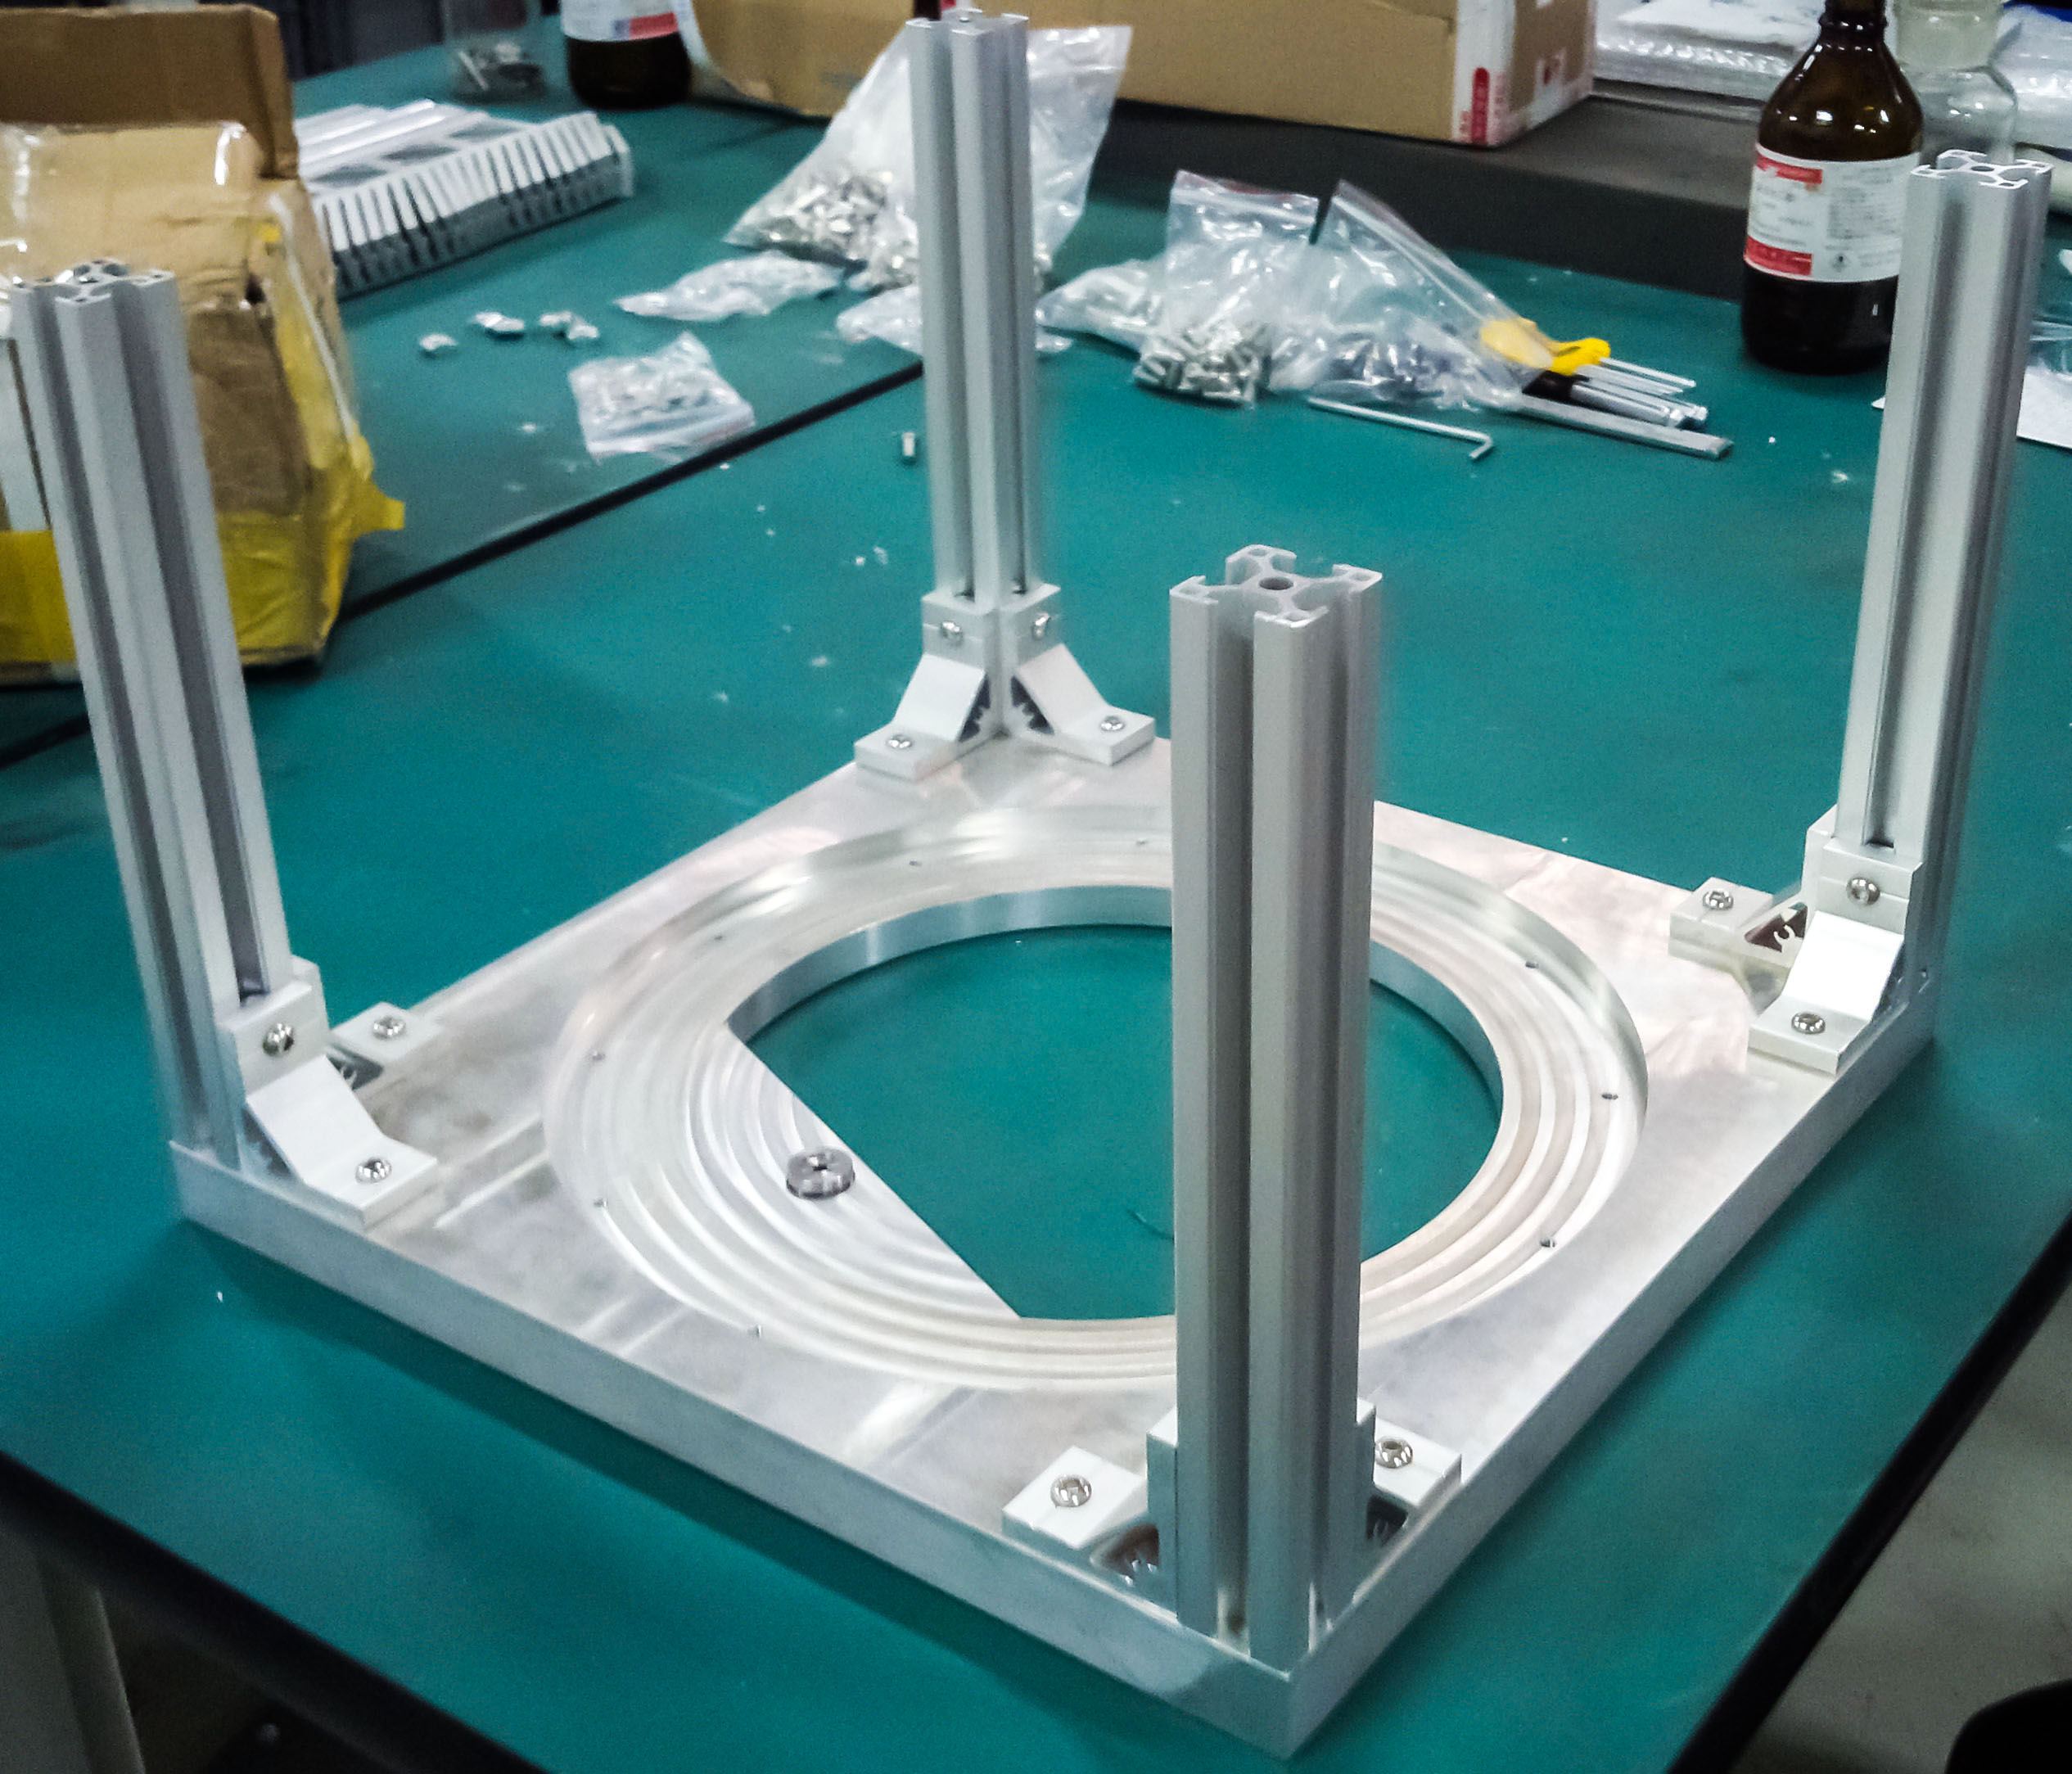
\includegraphics
      [max size={1\textwidth}{0.45\textheight}]
      {impl/mech__frame__assy__1.jpg}
    \caption{在连接板一侧连接4根纵向型材}
    \label{fig:impl-mech-frame-assy-sub1}
  \end{subfigure}
  \par\bigskip
  \begin{subfigure}{1\textwidth}
    \centering
    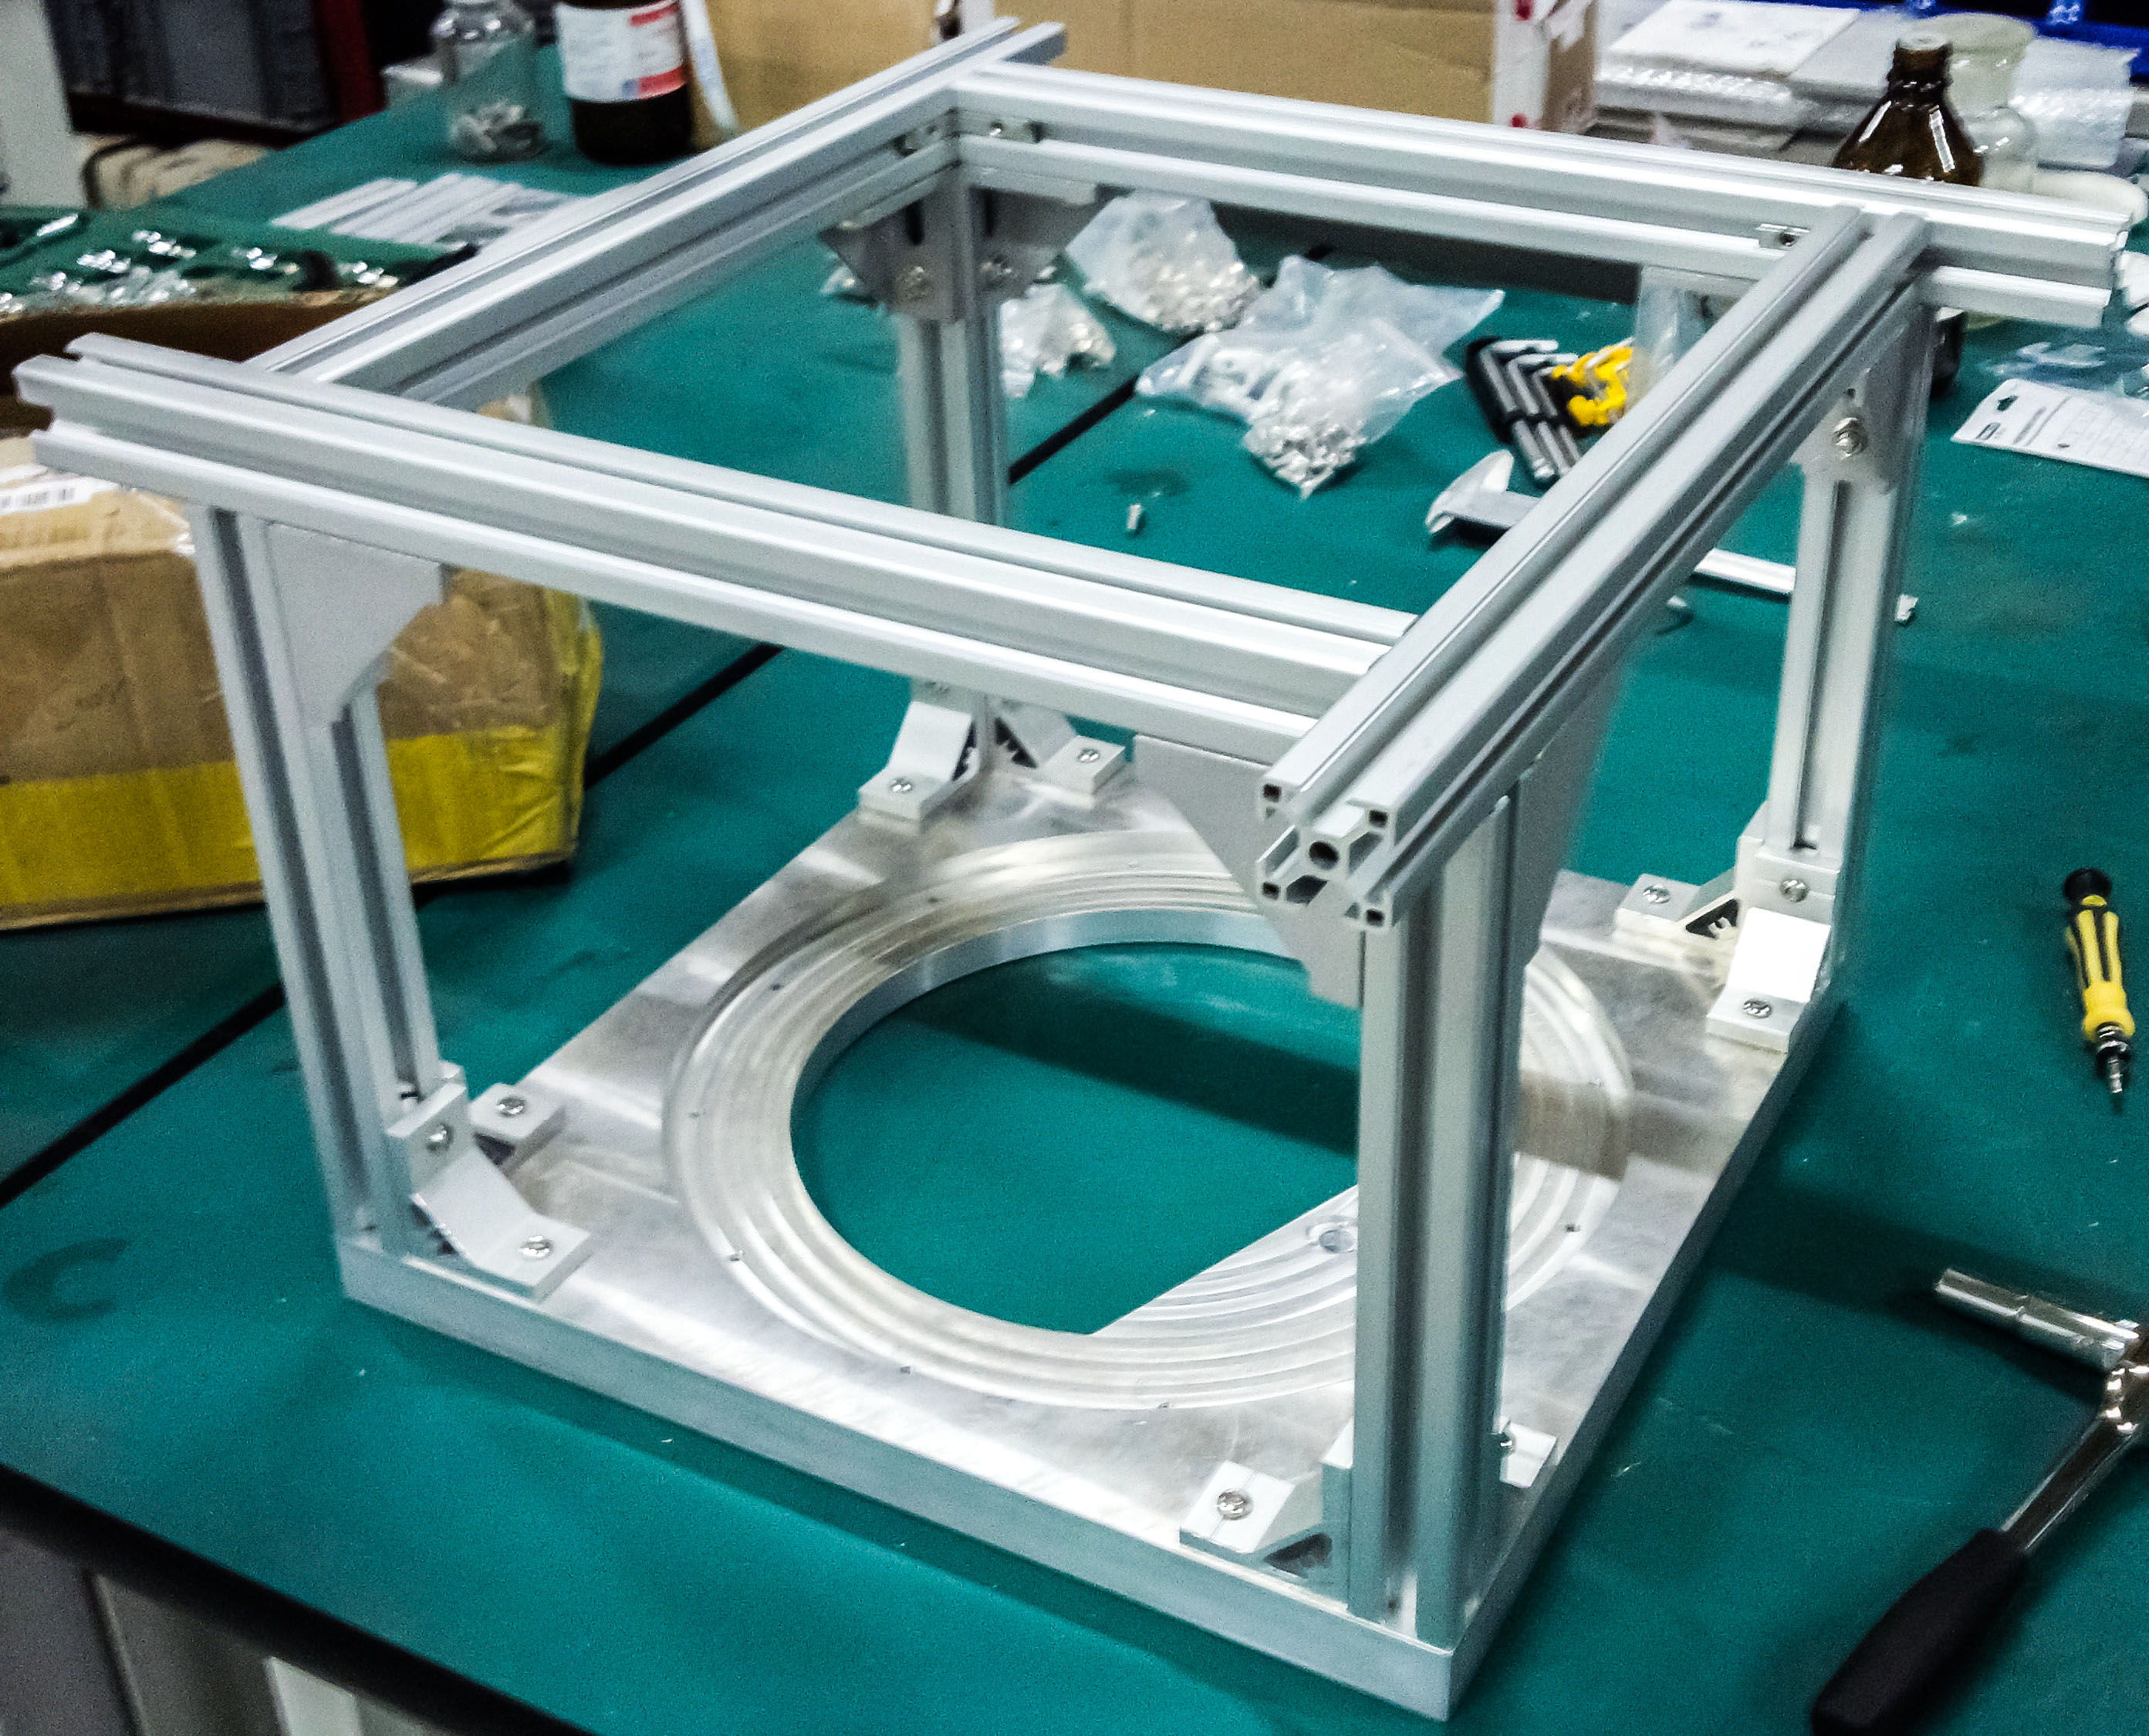
\includegraphics
      [max size={1\textwidth}{0.45\textheight}]
      {impl/mech__frame__assy__2.jpg}
    \caption{在纵向型材上完成正方形框架}
    \label{fig:impl-mech-frame-assy-sub2}
  \end{subfigure}
  \caption{框架结构主体装配实物图}
  \label{fig:impl-mech-frame-assy-a}
\end{figure}
\begin{figure}[p]
  \ContinuedFloat
  \centering
  \begin{subfigure}{1\textwidth}
    \centering
    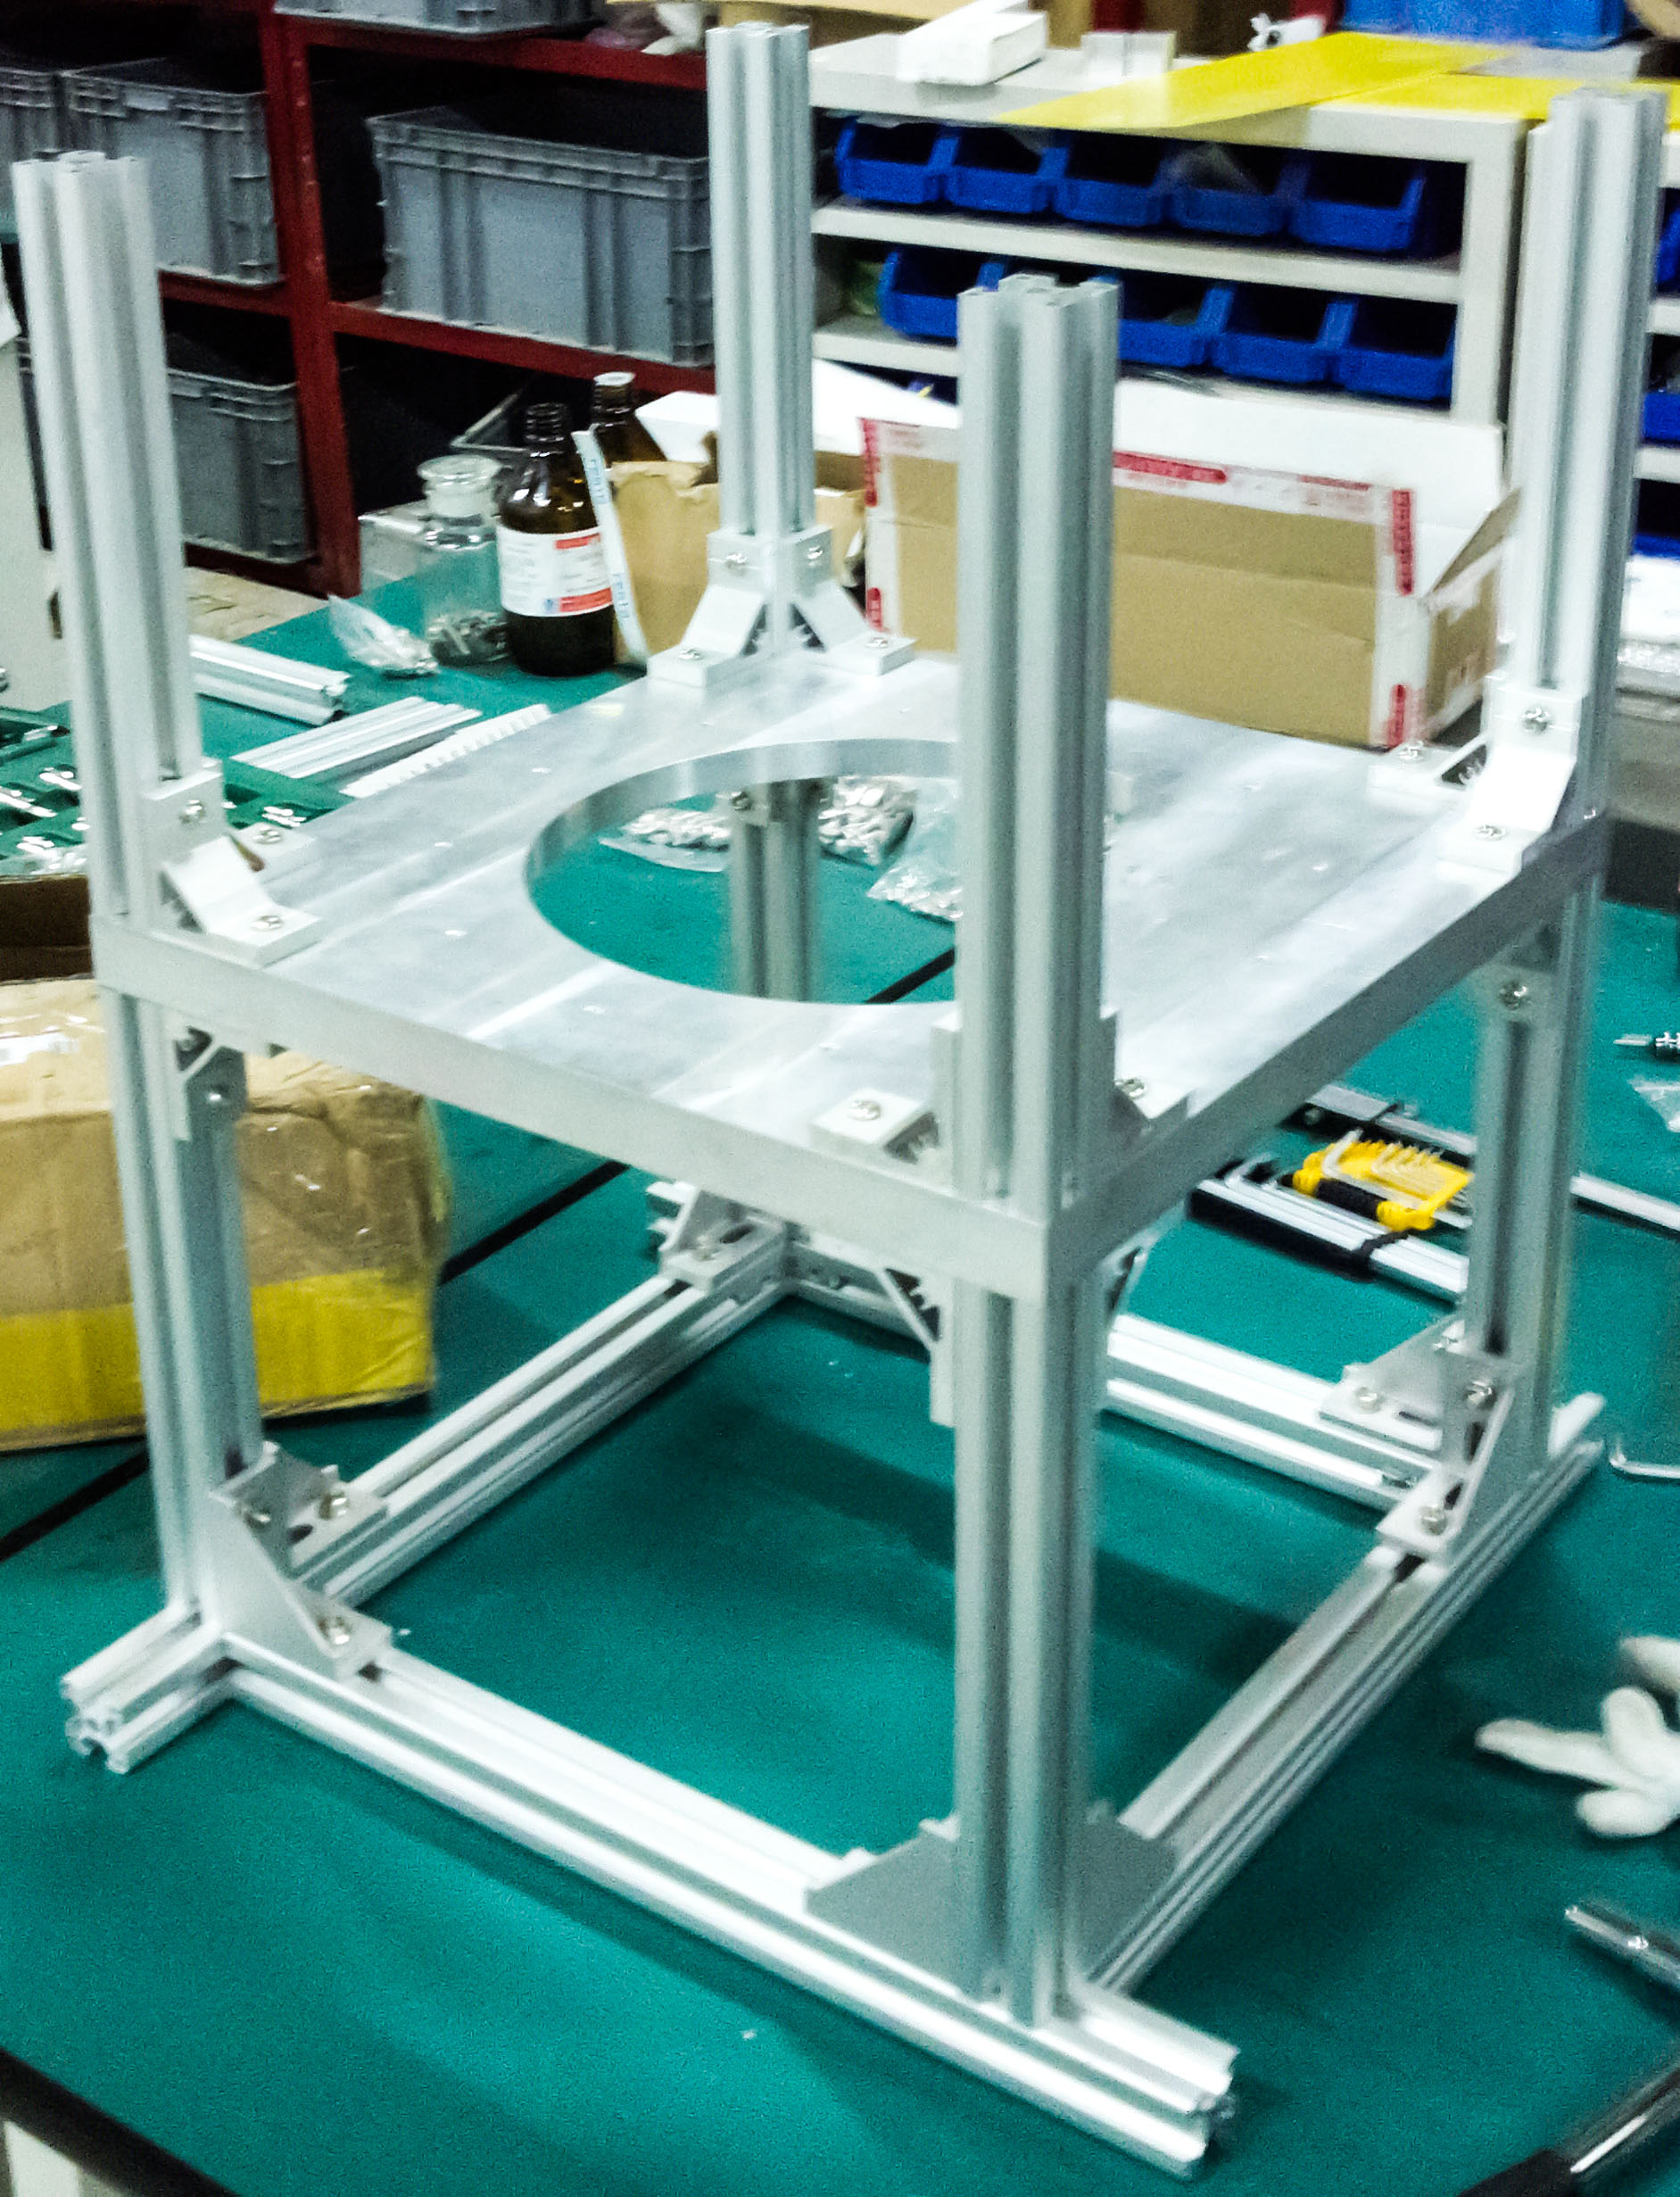
\includegraphics
      [max size={1\textwidth}{0.9\textheight}]
      {impl/mech__frame__assy__3.jpg}
    \caption{整体反转并连接另一侧的4根纵向型材}
    \label{fig:impl-mech-frame-assy-sub3}
  \end{subfigure}
  \caption{框架结构主体装配实物图(续1)}
  \label{fig:impl-mech-frame-assy-b}
\end{figure}
\begin{figure}[p]
  \ContinuedFloat
  \centering
  \begin{subfigure}{1\textwidth}
    \centering
    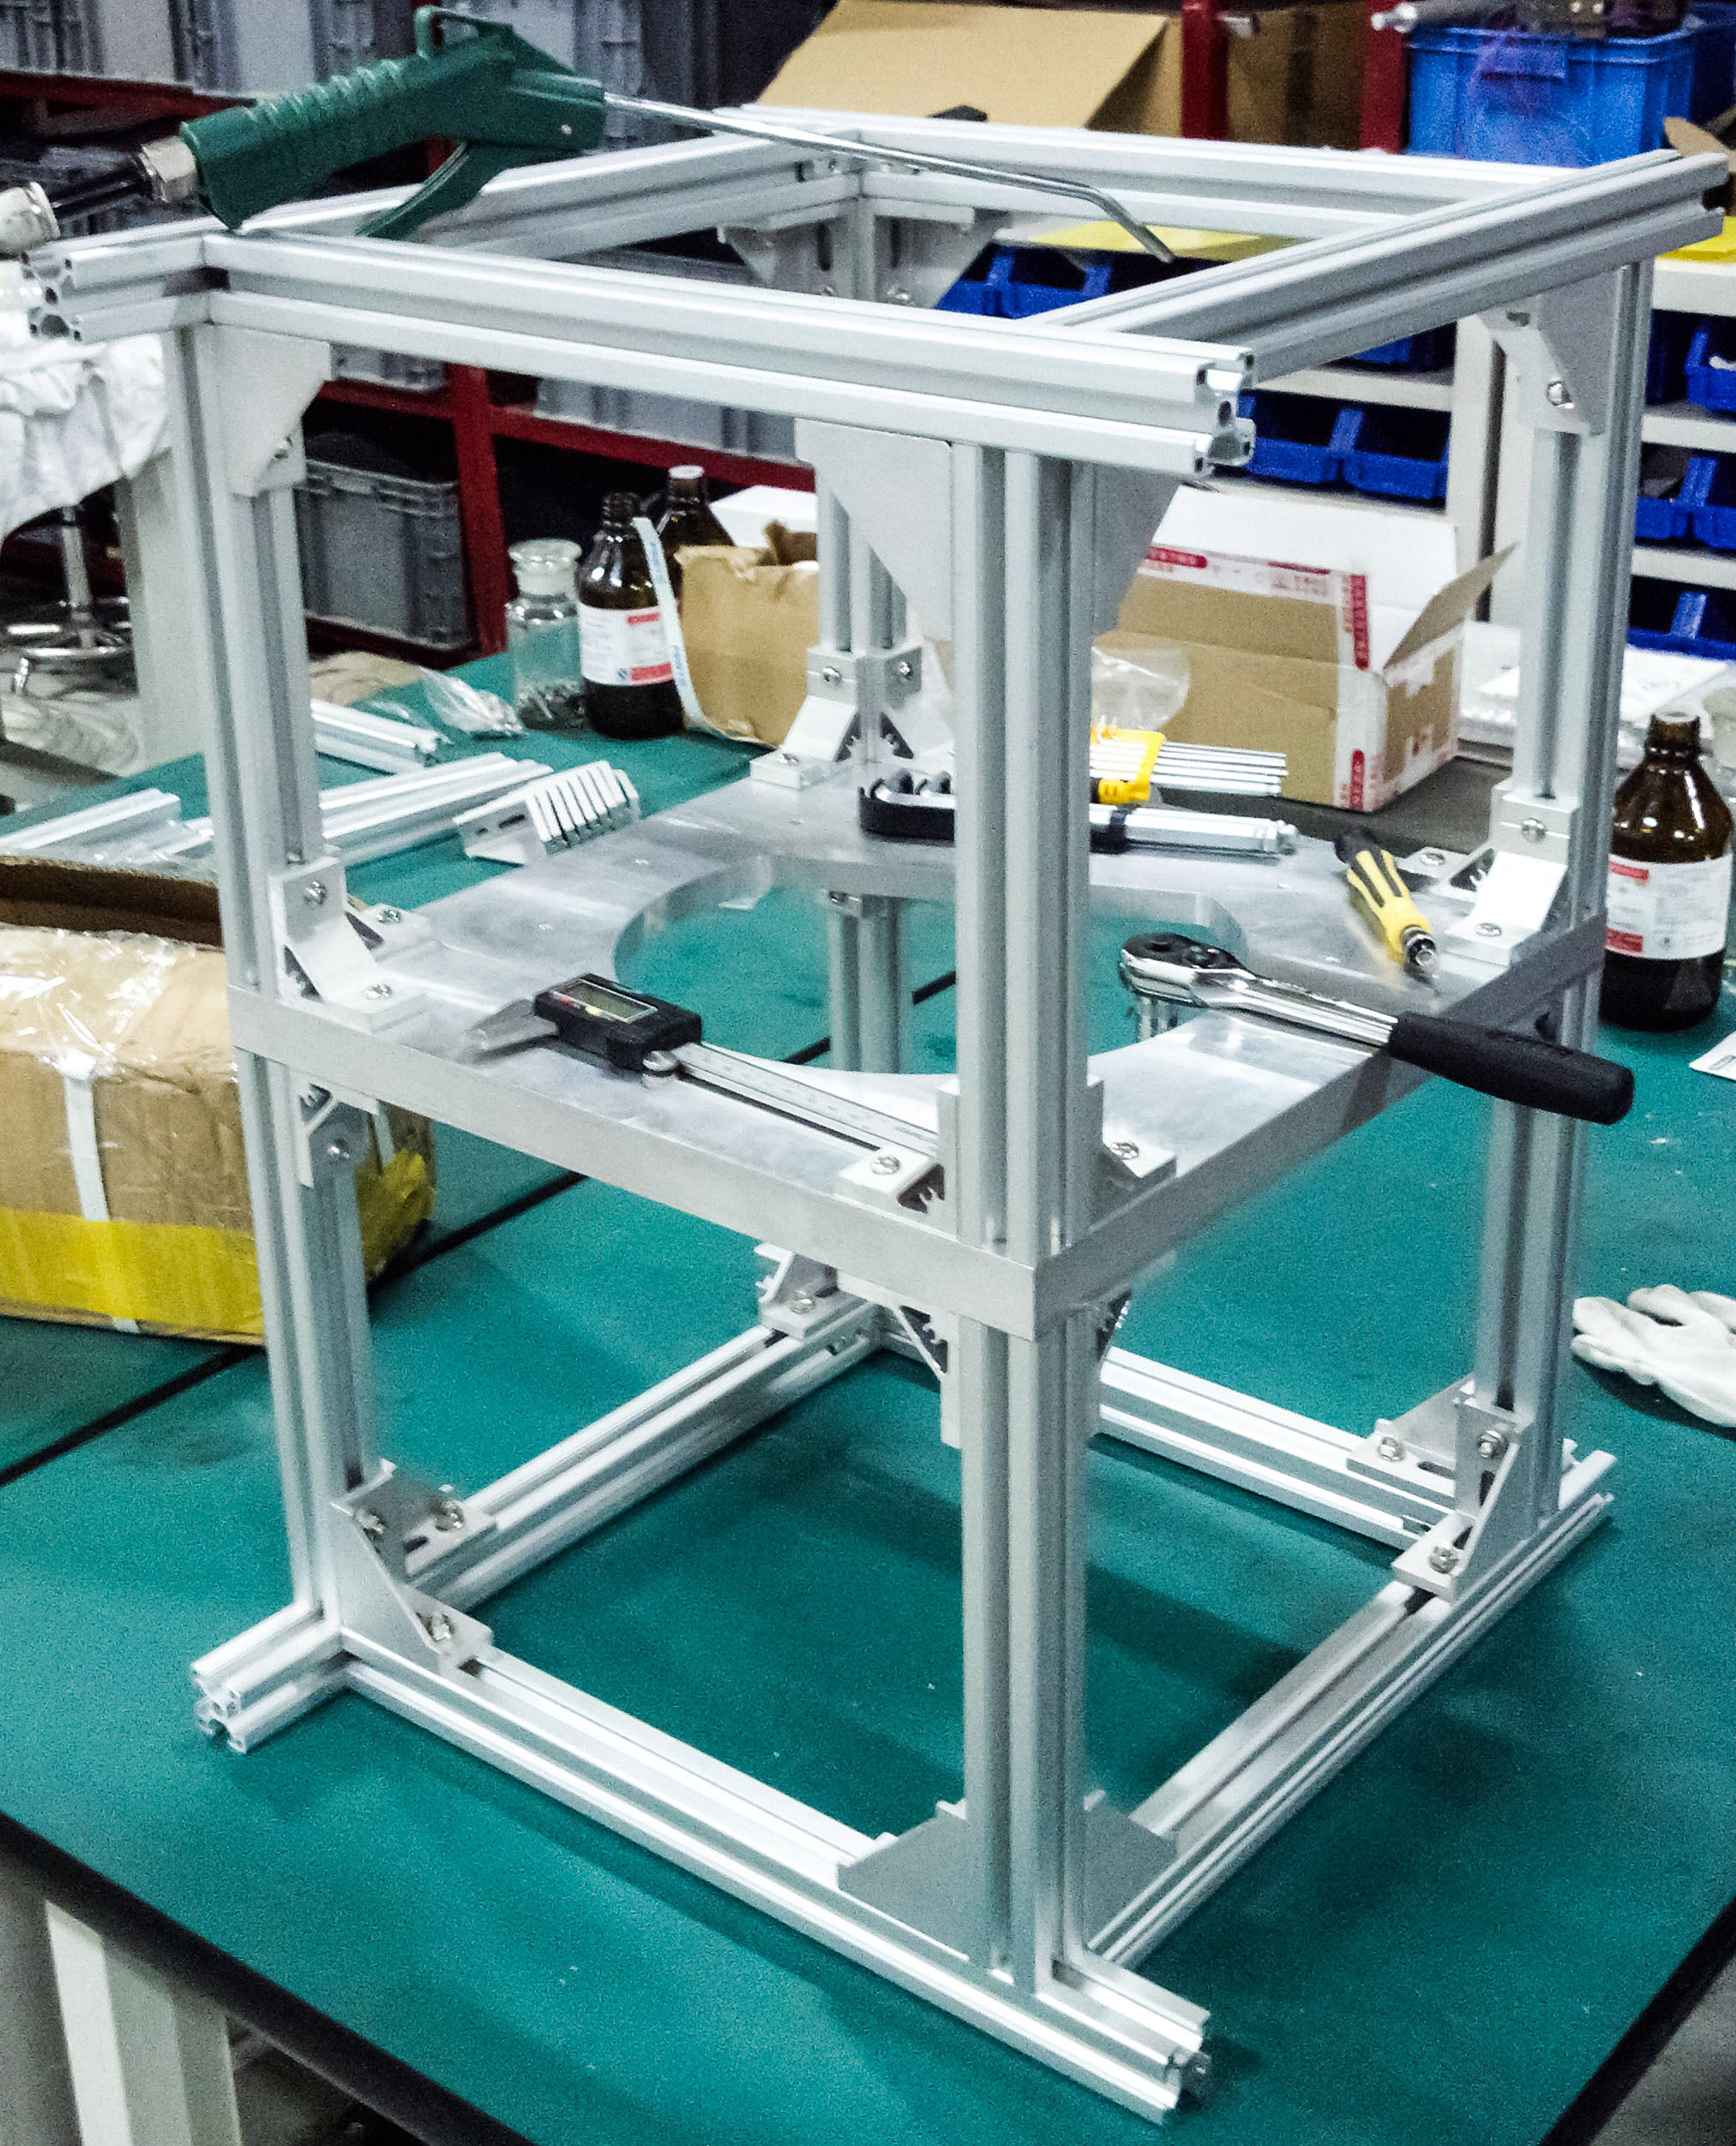
\includegraphics
      [max size={1\textwidth}{0.9\textheight}]
      {impl/mech__frame__assy__4.jpg}
    \caption{完成}
    \label{fig:impl-mech-frame-assy-sub4}
  \end{subfigure}
  \caption{框架结构主体装配实物图(续2)}
  \label{fig:impl-mech-frame-assy-c}
\end{figure}


\subsection{静电卡盘及其密封装配}\label{sec:impl-mech-chuck}

完成框架结构主体后,即可将静电卡盘装配到连接板上。为方便操作,可先将装配好的上层框架整体从静电卡盘连接板上暂时拆下,等静电卡盘完全装配好后再装回。装配方法如下:首先将选用的标准O型圈放入\ref{sec:rig-model-base}节中设计的密封接头中,再将密封接头插入静电卡盘连接板上与其配合的孔中,旋入三个紧定螺钉,使其刚好接触密封接头;然后,在固定住密封接头上端的同时,将标准M5气动快装接头旋入密封接头下端M5内螺纹孔\footnotemark{},用扳手将其旋紧;接下来将静电卡盘轻轻放在连接板上,对齐螺纹孔与沉孔后,用12个M5内六角螺钉将其固定在连接板上;最后,逐步、对称地旋紧三个紧定螺钉,使密封接头上表面与静电卡盘下表面良好接触,O型圈挤压到位,形成良好的端面密封。装配完成后如图~\ref{fig:impl-mech-chuck}。

\footnotetext{所有气动接头均需使用聚四氟乙烯生料带保证密封,下略。}

\begin{figure}[p]
  \centering
  \begin{subfigure}{1\textwidth}
    \centering
    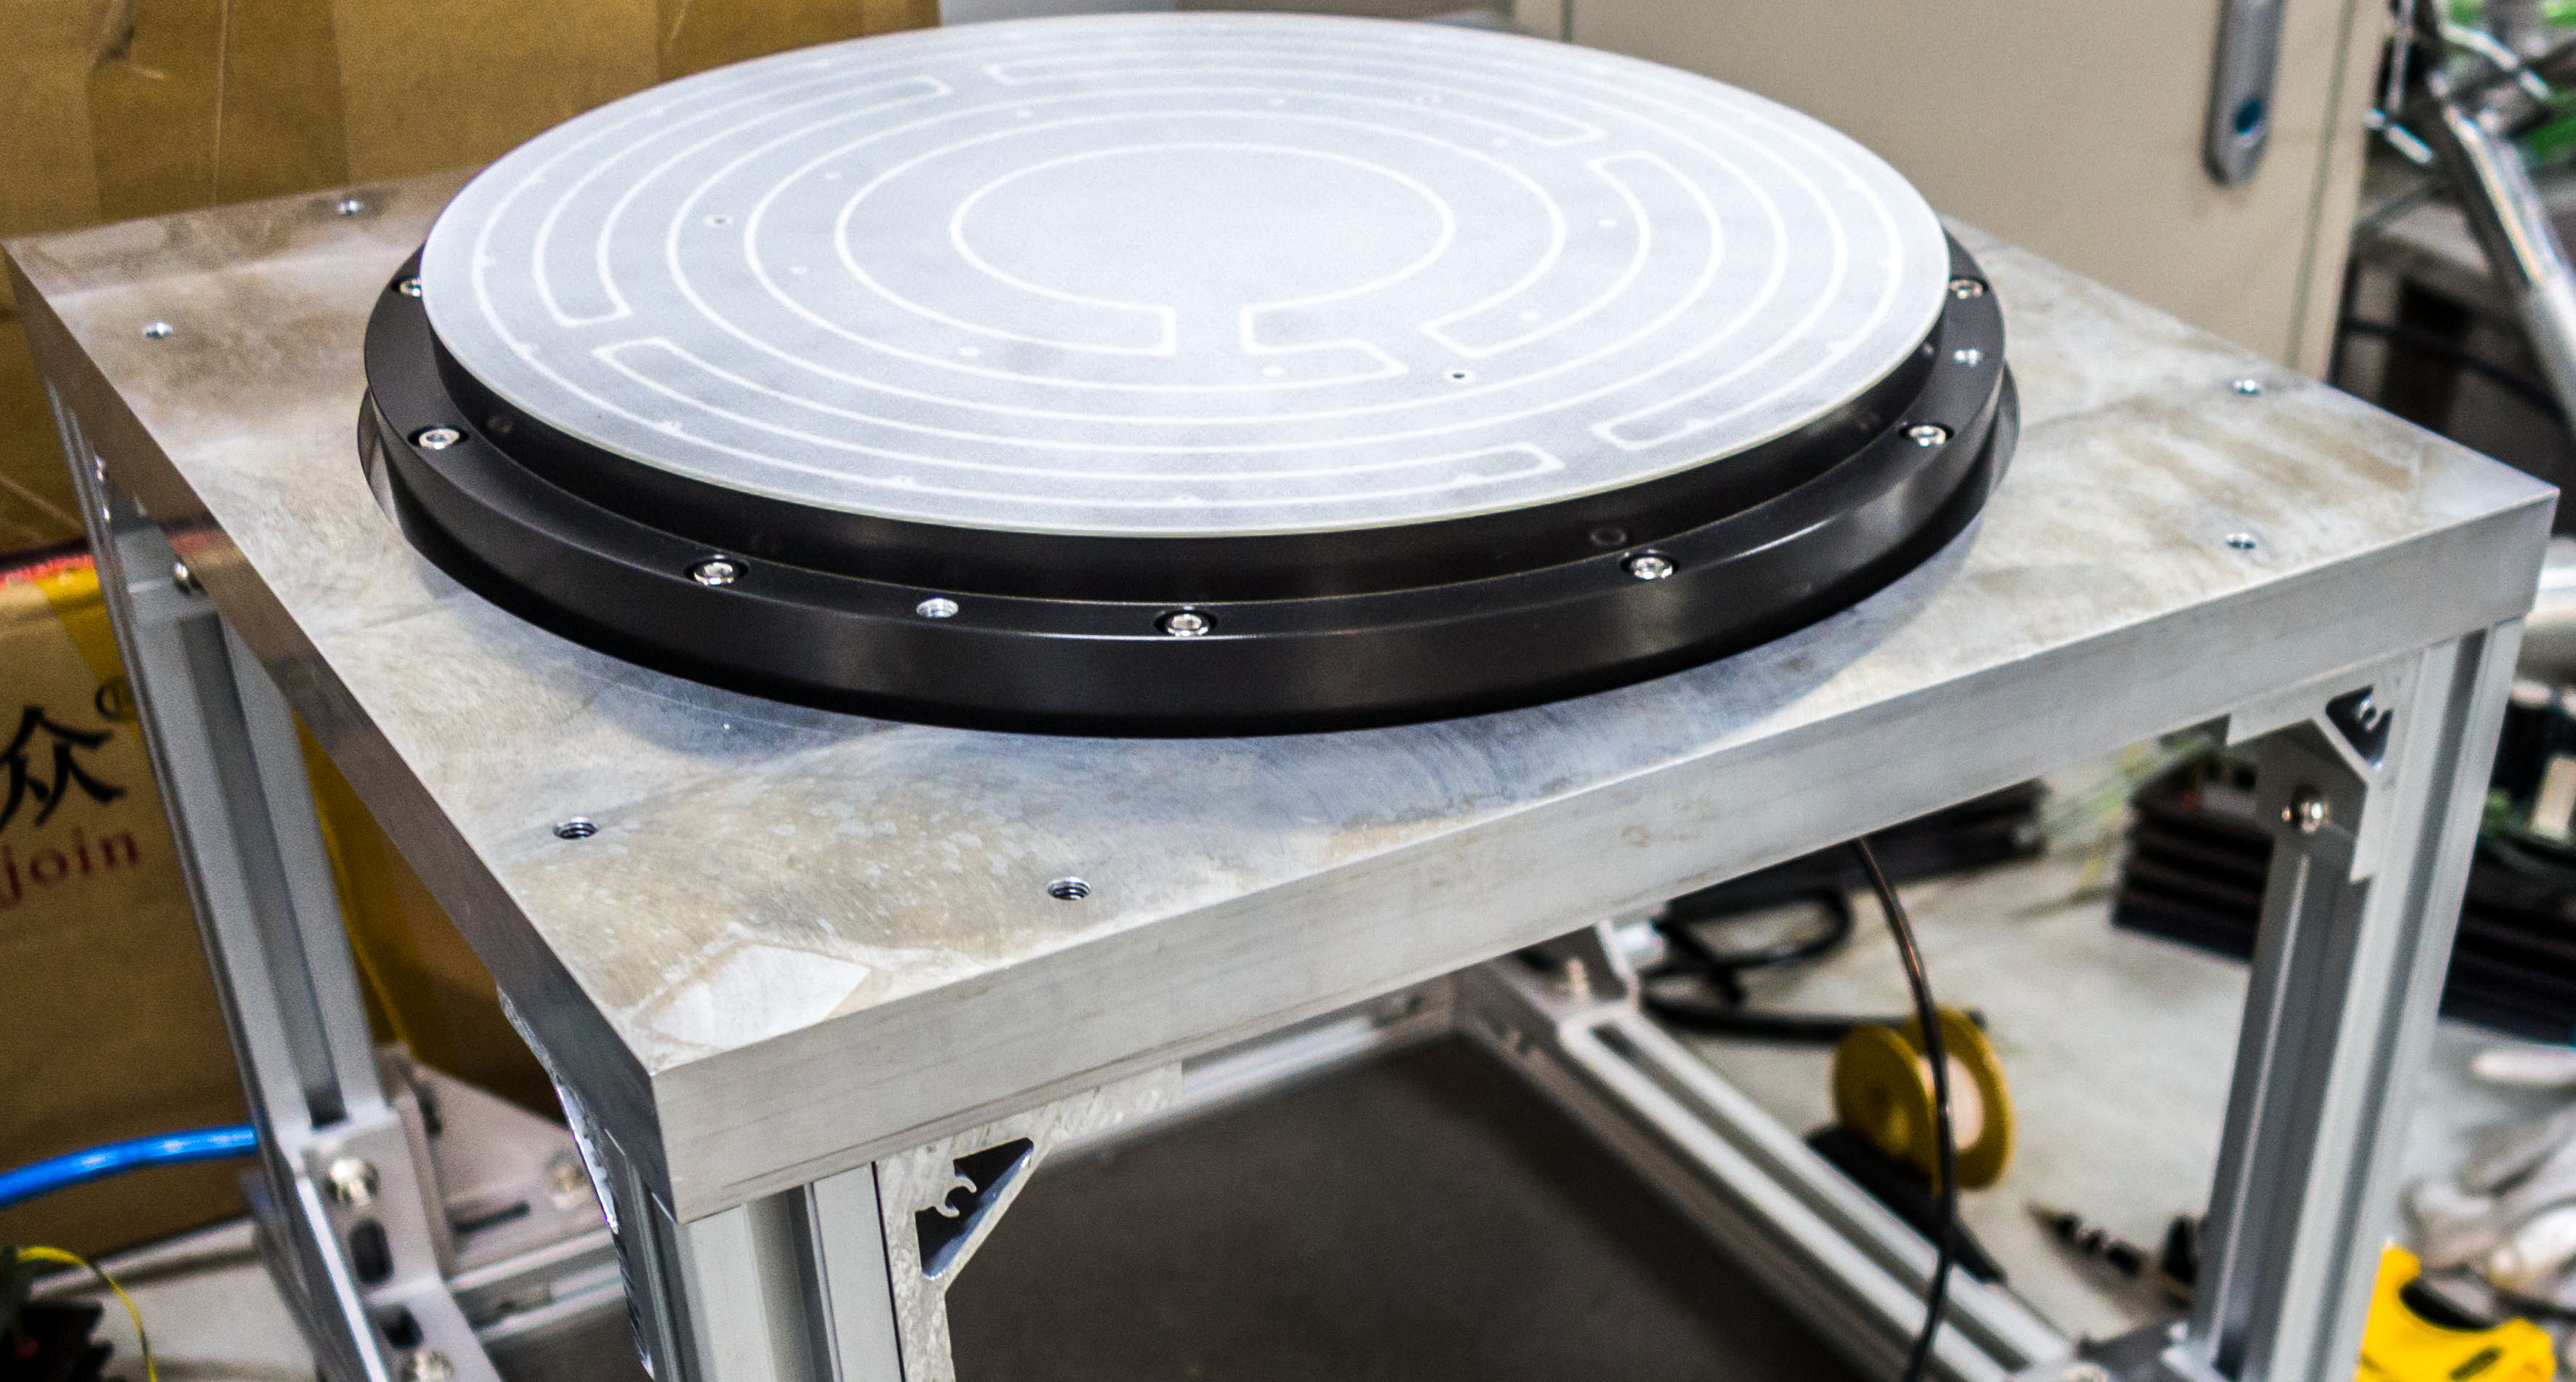
\includegraphics
      [max size={1\linewidth}{0.45\textheight}]
      {impl/mech__chuck__top.jpg}
    \caption{顶部(上层框架已拆除)}
    \label{fig:impl-mech-chuck-top}
  \end{subfigure}
  \par\bigskip
  \begin{subfigure}{1\textwidth}
    \centering
    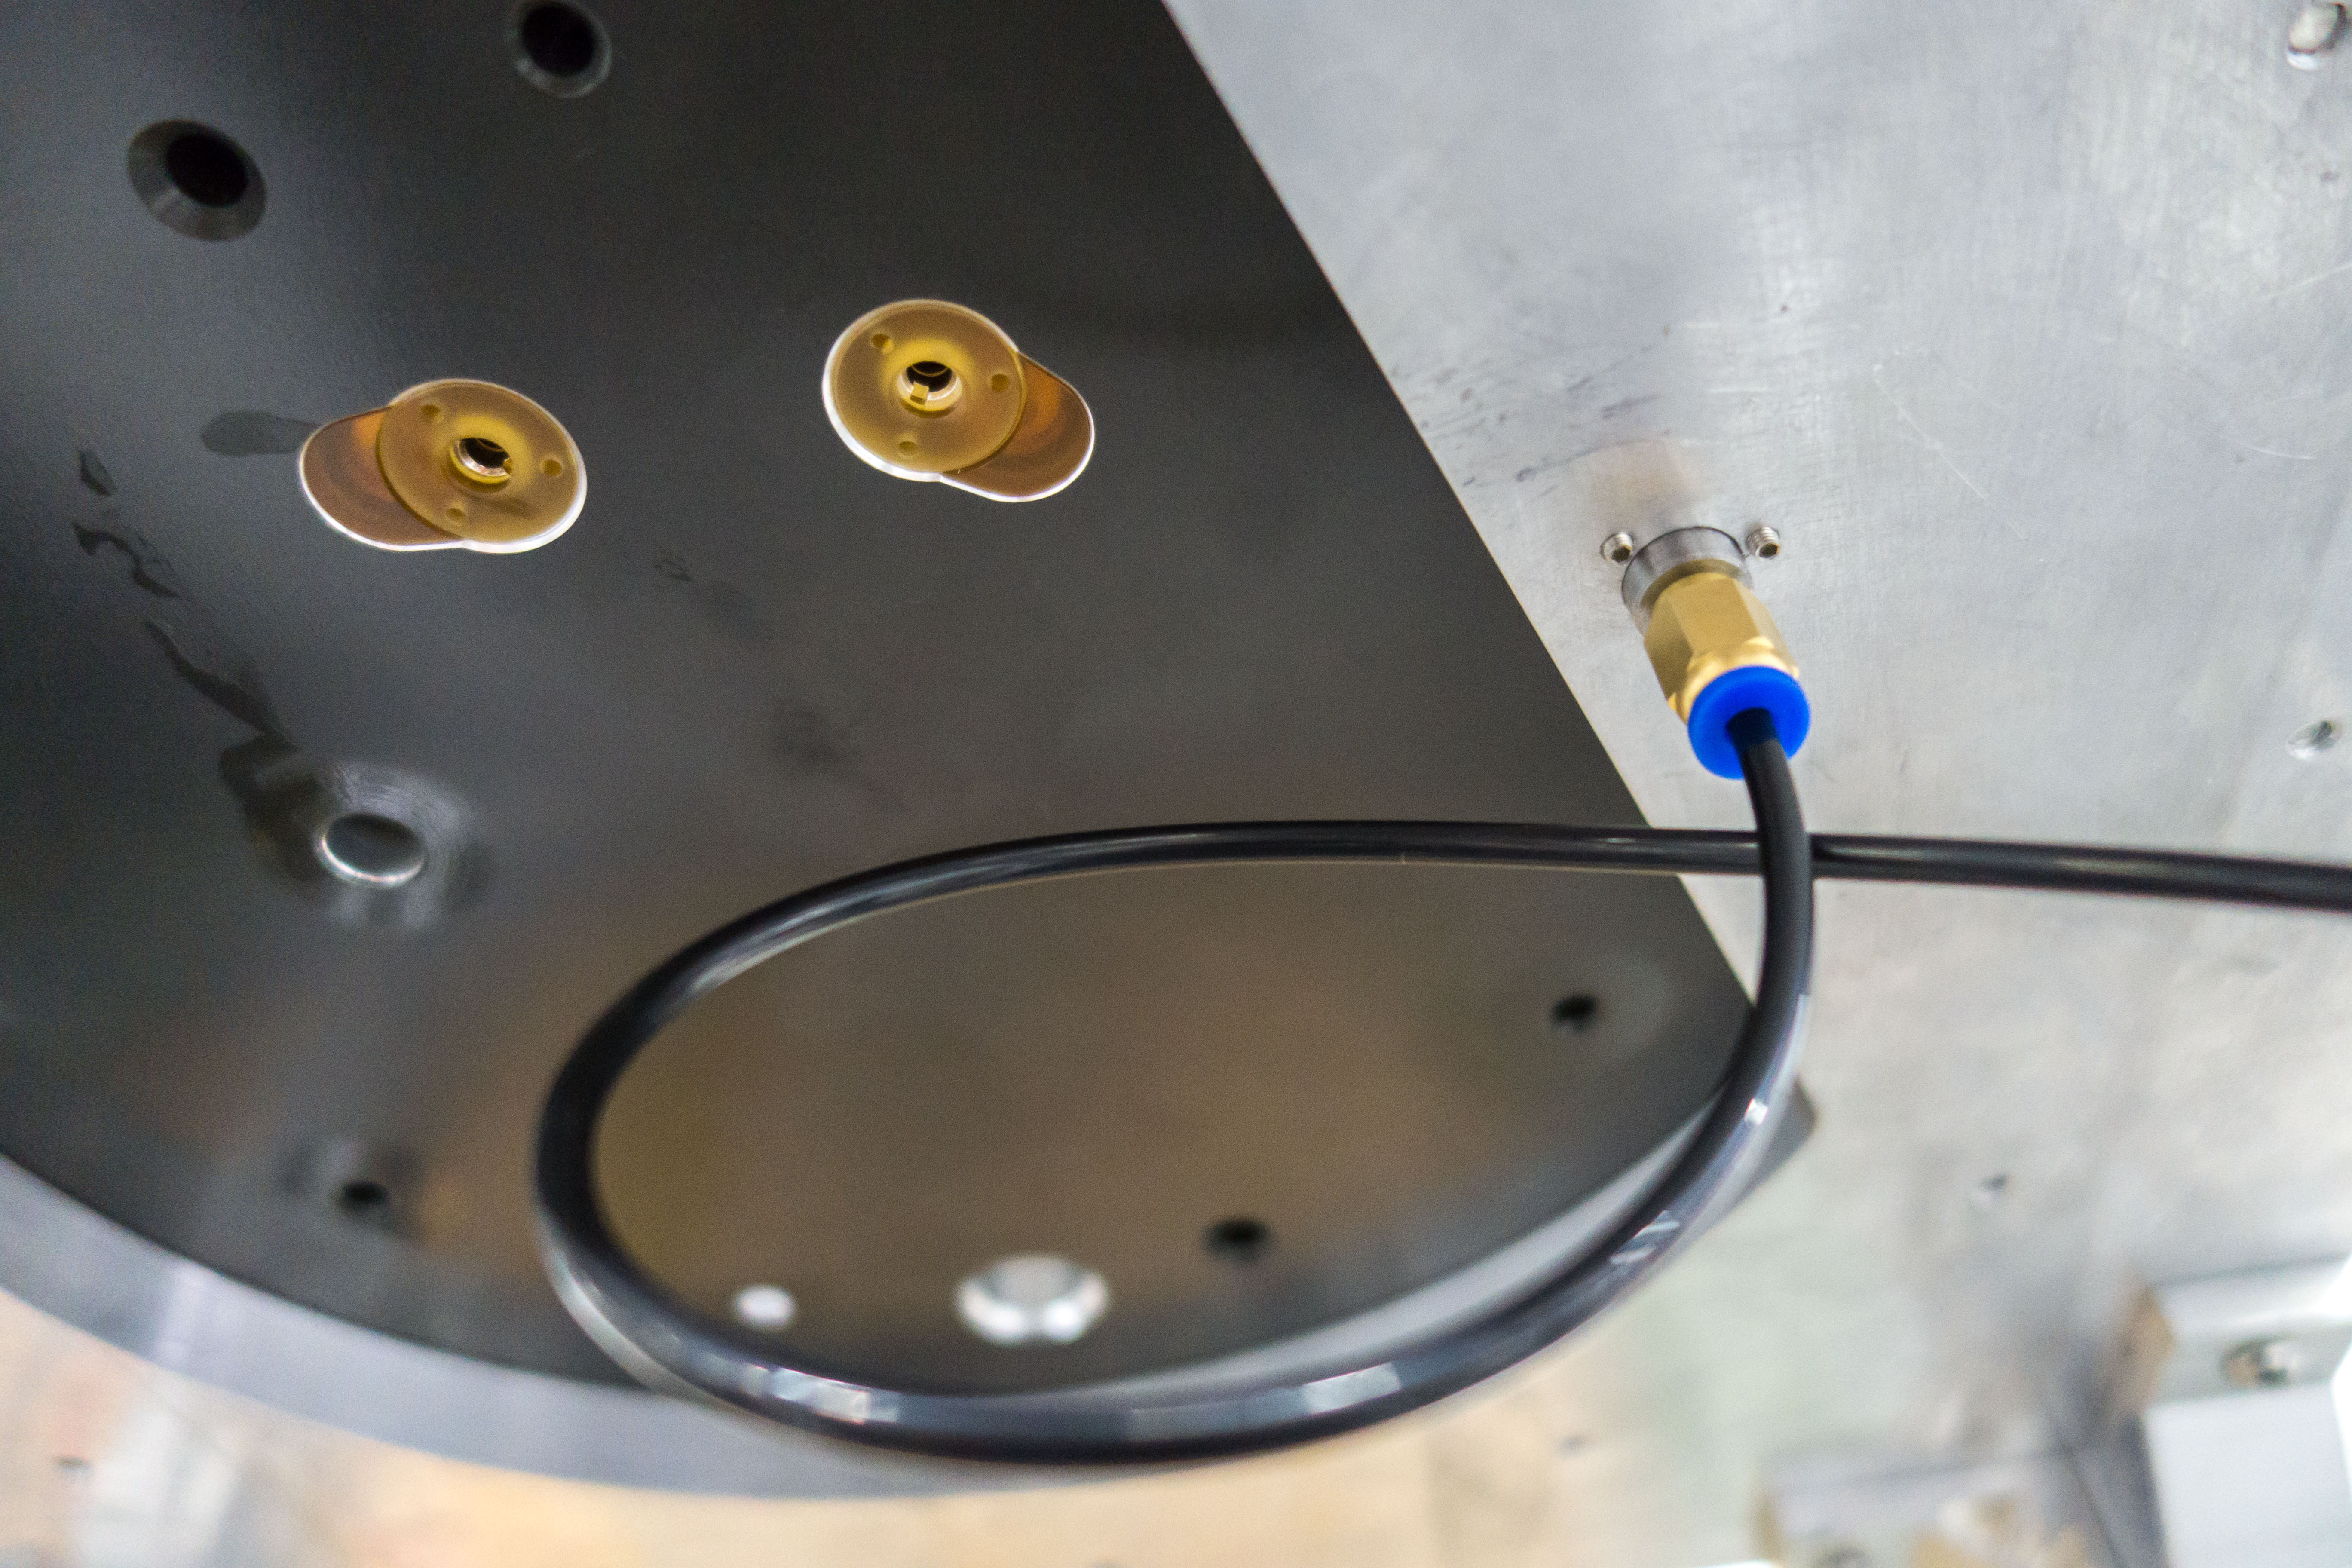
\includegraphics
      [max size={1\linewidth}{0.45\textheight}]
      {impl/mech__chuck__bottom.jpg}
    \caption{底部}
    \label{fig:impl-mech-chuck-bottom}
  \end{subfigure}
  \caption{静电卡盘装配实物图}
  \label{fig:impl-mech-chuck}
\end{figure}


\subsection{微力探头组件}\label{sec:impl-mech-probe}

由于LSB200微力传感器安全过载仅\SI{1}{\newton},装配时应小心避免对其造成不可恢复的损伤,尤其是当需要用手触碰到其活动端时。具体装配方法如下:

\begin{enumerate}
  \item
    将LSB200接入电控系统,并在整个装配过程中监测其读数,避免其受力超过满量程。
  \item
    轻轻握住LSB200活动端,使其外壳贴有商标的一面朝上,将螺纹转接头(\ref{sec:rig-model-probe}节)的M3外螺纹端轻轻旋入LSB200活动端,并在保证LSB200不过载的同时,将转接头旋紧。
  \item
    用小钳子夹住转接头,将红宝石探头旋入螺纹转接头的M2内螺纹端。
  \item
    使LAC-10A/JYPY-02213处于伸长状态,轻轻握住传感器侧面(固定端),将其连接在推杆末端/平移台上。
  \item
    将LAC-10A/JYPY-02213固定在连接板上。
\end{enumerate}

之后,可按一般型材装配方式组装\ref{sec:rig-model-probe}节中设计的粗调框架,并将微力探头连接板通过T槽螺母与内六角螺栓紧固在其上。装配完成后如图~\ref{fig:impl-pcb-zaber-new-photo}。

\begin{figure}[p]
\centering
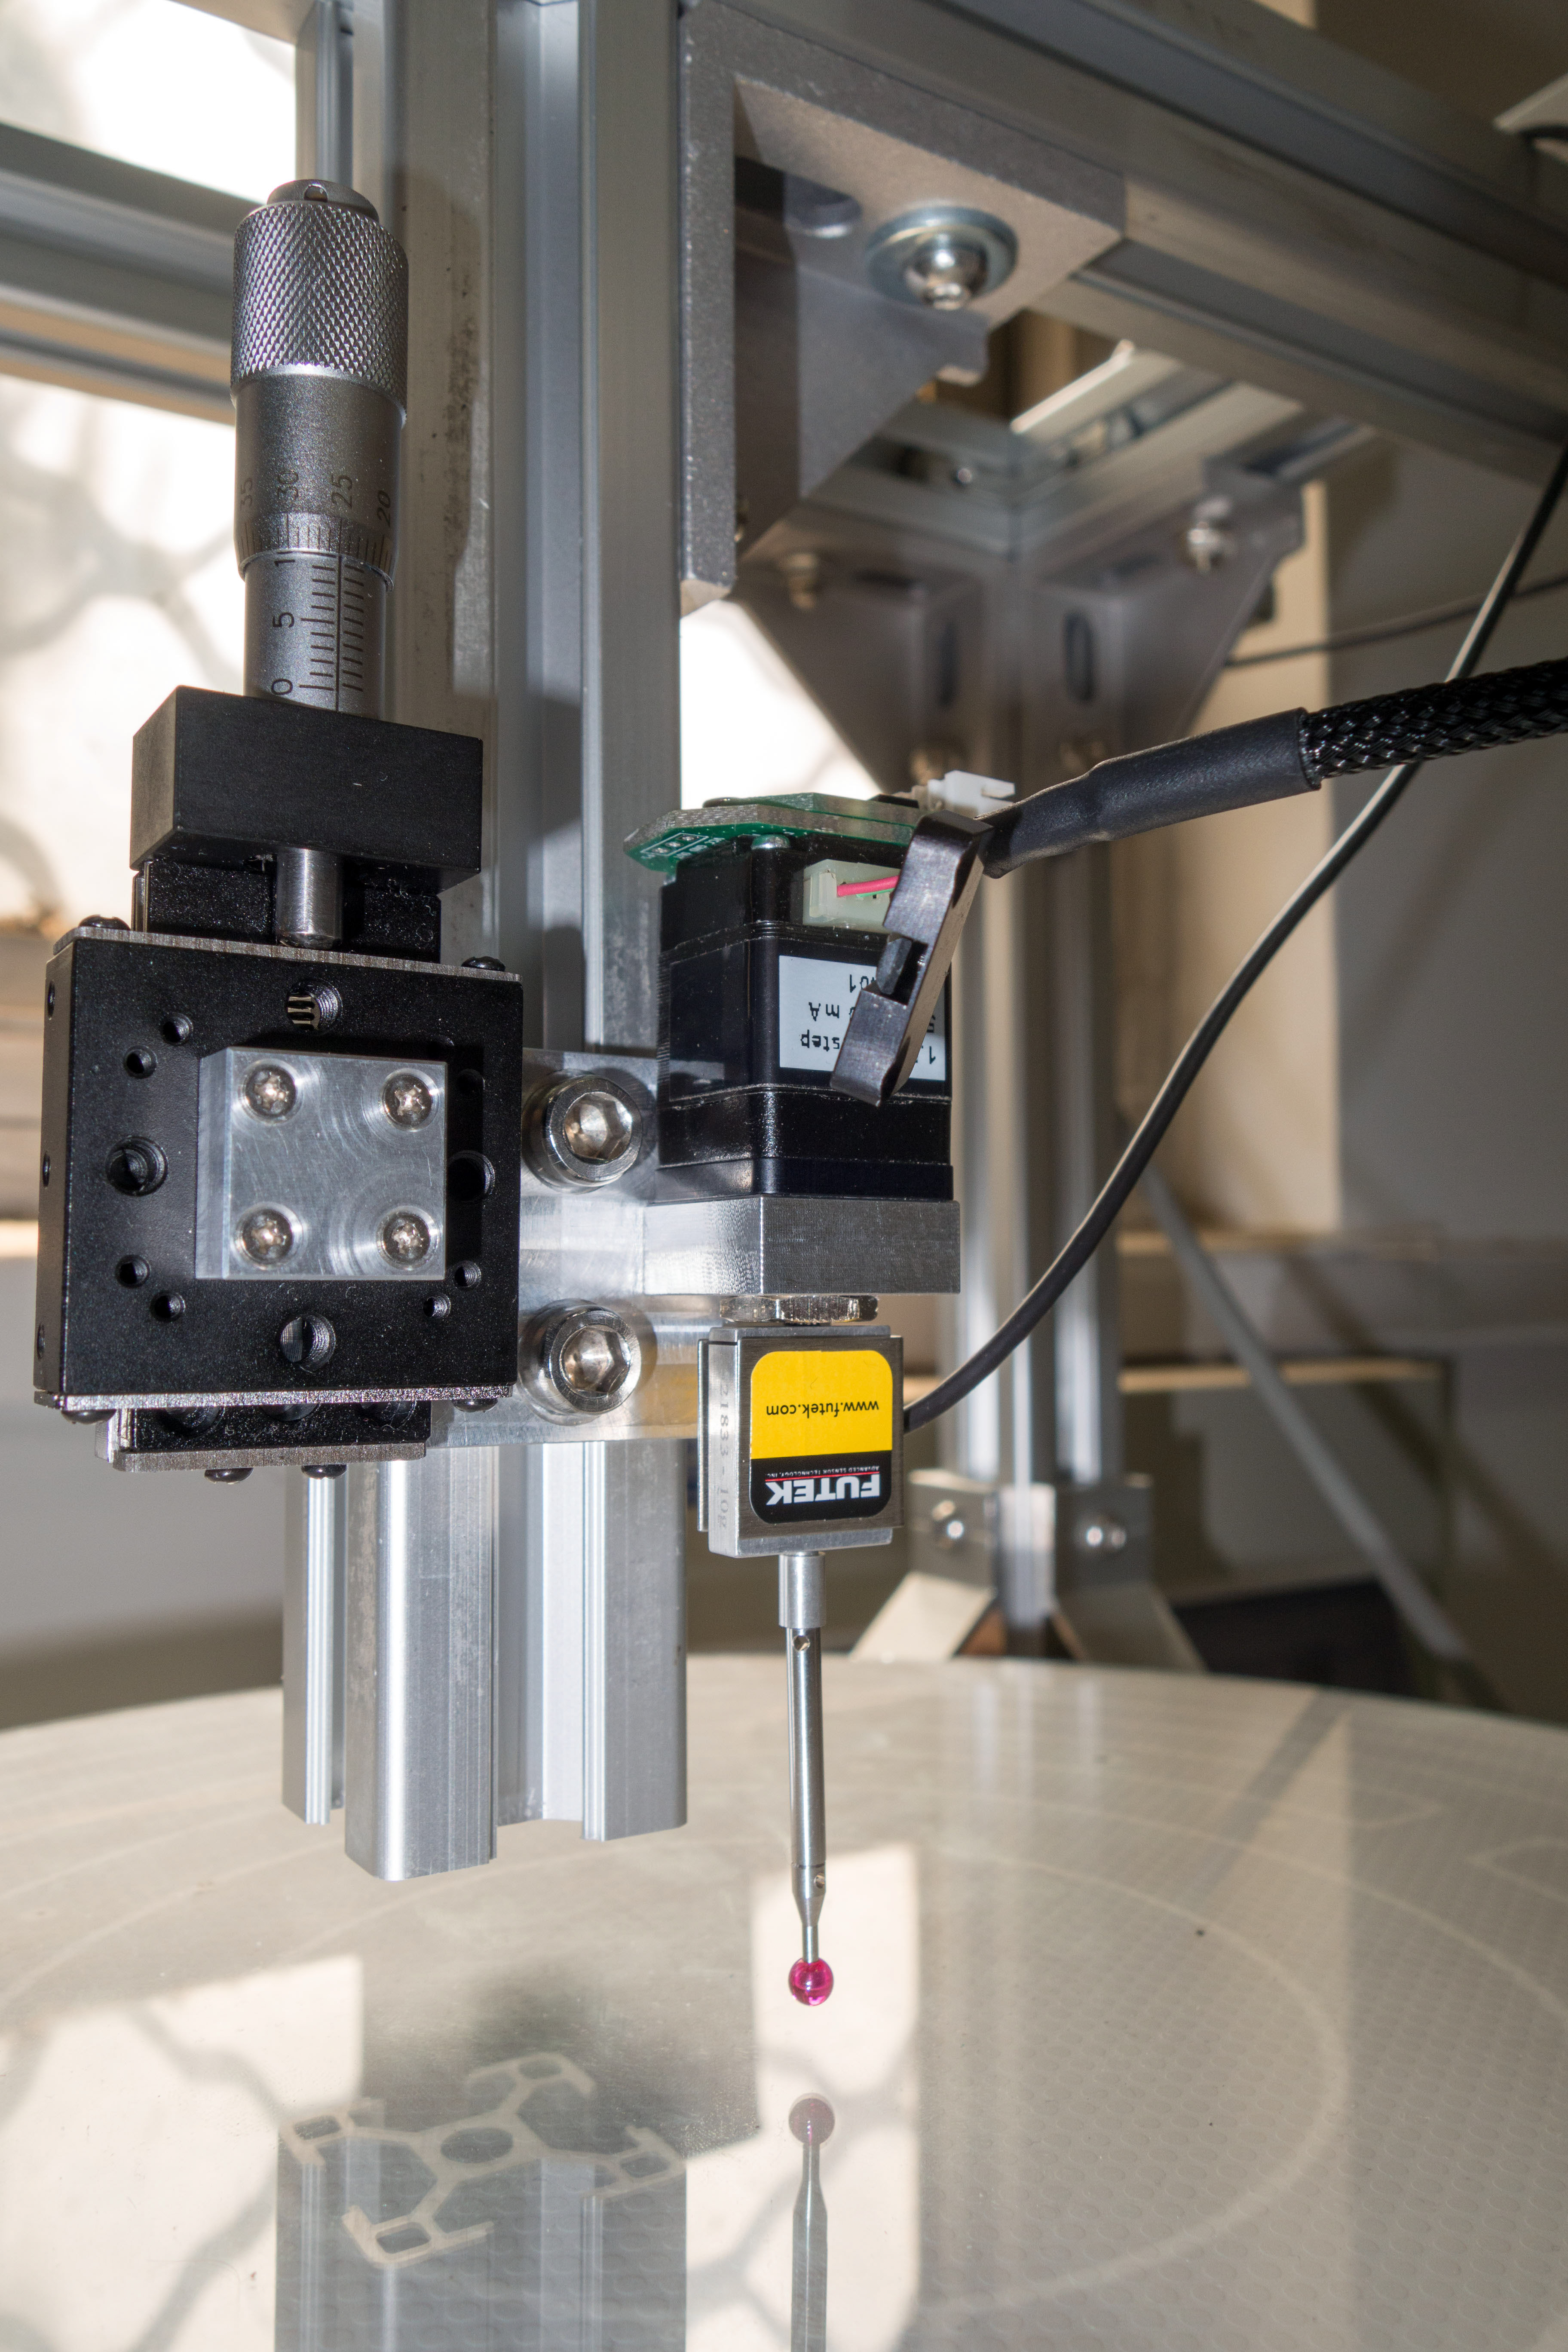
\includegraphics
  [max size={1\linewidth}{1\textheight}]
  {impl/mech__probe__assy.jpg}
\caption{微力探头组件实物图}
\label{fig:impl-mech-probe-assy}
\end{figure}



\clearpage



\section{电路实现与调试}\label{sec:impl-pcb}

本节讨论\ref{sec:rig-ctrl}节电控系统中所有自行设计的电子模块的具体实现,主要包括万用板、PCB的设计与制作,电路的调试以及性能测试等。


\subsection{背吹控制系统接口}\label{sec:impl-pcb-pressure}

由于背吹控制系统中的元件(压强变送器、电子比例阀、电磁方向阀)在试验台中较为接近(均可布置在底部),且均需要较高电压的直流电源(\SI{+24}{\V}与\SI{+12}{\V}),可将这三部分的接口电路集成在同一块PCB上。总体设计如图~\ref{fig:impl-pcb-pressure-sch-overall}:\SI{+24}{\V}单电源供电,通过稳压电路(``power'')获得其他所需电压;其他部分(\SIrange{4}{20}{\mA}电流环接口等)原理见\ref{sec:rig-ctrl}节。共使用4个标准可插拔式接线端子:\bverb|P1|接电源输入、\bverb|P2|接电流环、\bverb|P4|接电磁方向阀、\bverb|P5|接电子比例阀。\bverb|P5|接MCU(数据、数字供电),选用标准10针简单牛角接头。

稳压电路拓扑结构如图~\ref{fig:impl-pcb-pressure-sch-power}:\SI{+24}{\V}电源输入首先通过电源滤波保护电路(``line filter''),然后依次经过两级线性稳压芯片得到\SI{+12}{\V}与\SI{+5}{\V};同时,\SI{+12}{\V}还向精密\SI{+5}{\V}电压基准芯片供电,以提供ADC所需要的参考电压。滤波保护电路原理如图~\ref{fig:impl-pcb-pressure-sch-power-filter}:\bverb|D1|为防反接二极管;\bverb|L1|、\bverb|L2|为磁珠,对高频信号呈阻性,用于衰减高频电源噪声;\bverb|T1|为共模电感,与\bverb|C2|、\bverb|C3|、\bverb|C4|形成LC滤波器,用于消除电源纹波;\bverb|D2|为TVS(瞬态电压抑制)二极管,可防止电压尖峰损坏电路。这样既可对整个PCB乃至外部元件起到保护作用,又可降低模拟电路中因电源纹波产生的噪声。需要注意的是,虽然设计了板载滤波电路,仍不应直接使用开关电源供电,最好先经过外置直流电源滤波器消除较高能量的纹波,再接入PCB。

上述设计为v0.3.1版本,之前设计的v0.2.1版本不含板载电源滤波器,且其中第一级稳压电路为DC-DC开关转换器,实测发现模拟信号噪声极大,其中含有周期性的纹波成分以及频繁的尖峰,如\ref{fig:impl-pcb-pressure-emi-before};加入滤波电路后,各种噪声均显著降低,如\ref{fig:impl-pcb-pressure-emi-after}。完成的v0.3.1版本电路如图~\ref{fig:impl-pcb-pressure-photo-pcb}。

\begin{figure}[hbp]
\centering
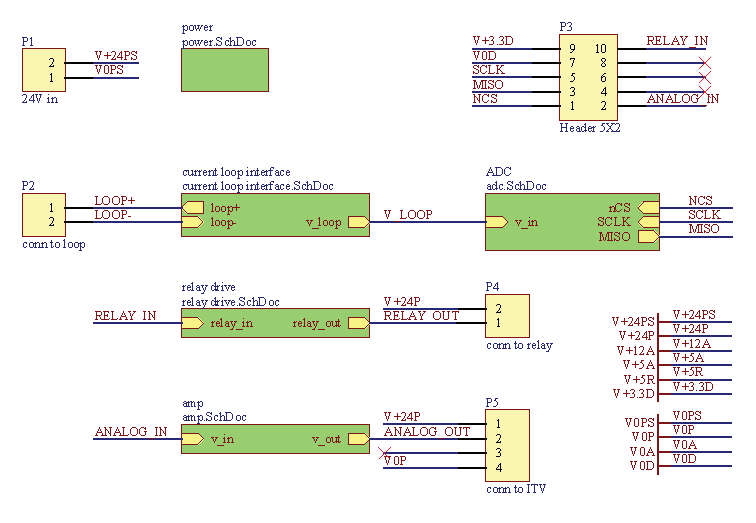
\includegraphics[width=0.87\linewidth]{impl/pcb__pressure__sch__overall}
\caption{背吹控制系统接口\csep 原理图\csep 总体}
\label{fig:impl-pcb-pressure-sch-overall}
\end{figure}

\begin{figure}[hbp]
\centering
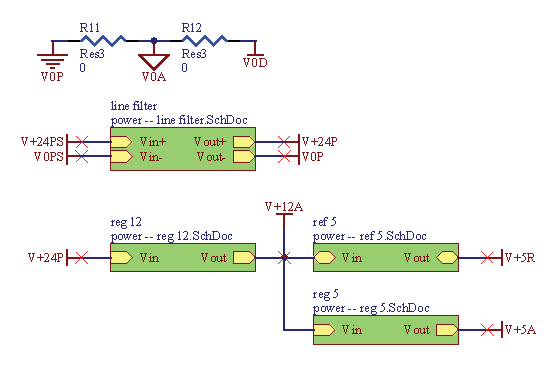
\includegraphics[width=0.65\linewidth]{impl/pcb__pressure__sch__power}
\caption{背吹控制系统接口\csep 原理图\csep 稳压}
\label{fig:impl-pcb-pressure-sch-power}
\end{figure}

\begin{figure}[p]
\centering
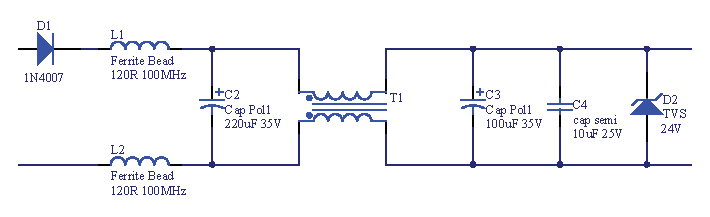
\includegraphics[width=0.90\linewidth]{impl/pcb__pressure__sch__power__filter}
\caption{背吹控制系统接口\csep 原理图\csep 滤波}
\label{fig:impl-pcb-pressure-sch-power-filter}
\end{figure}

\begin{figure}[p]
  \centering
  \begin{subfigure}{1\textwidth}
    \centering
    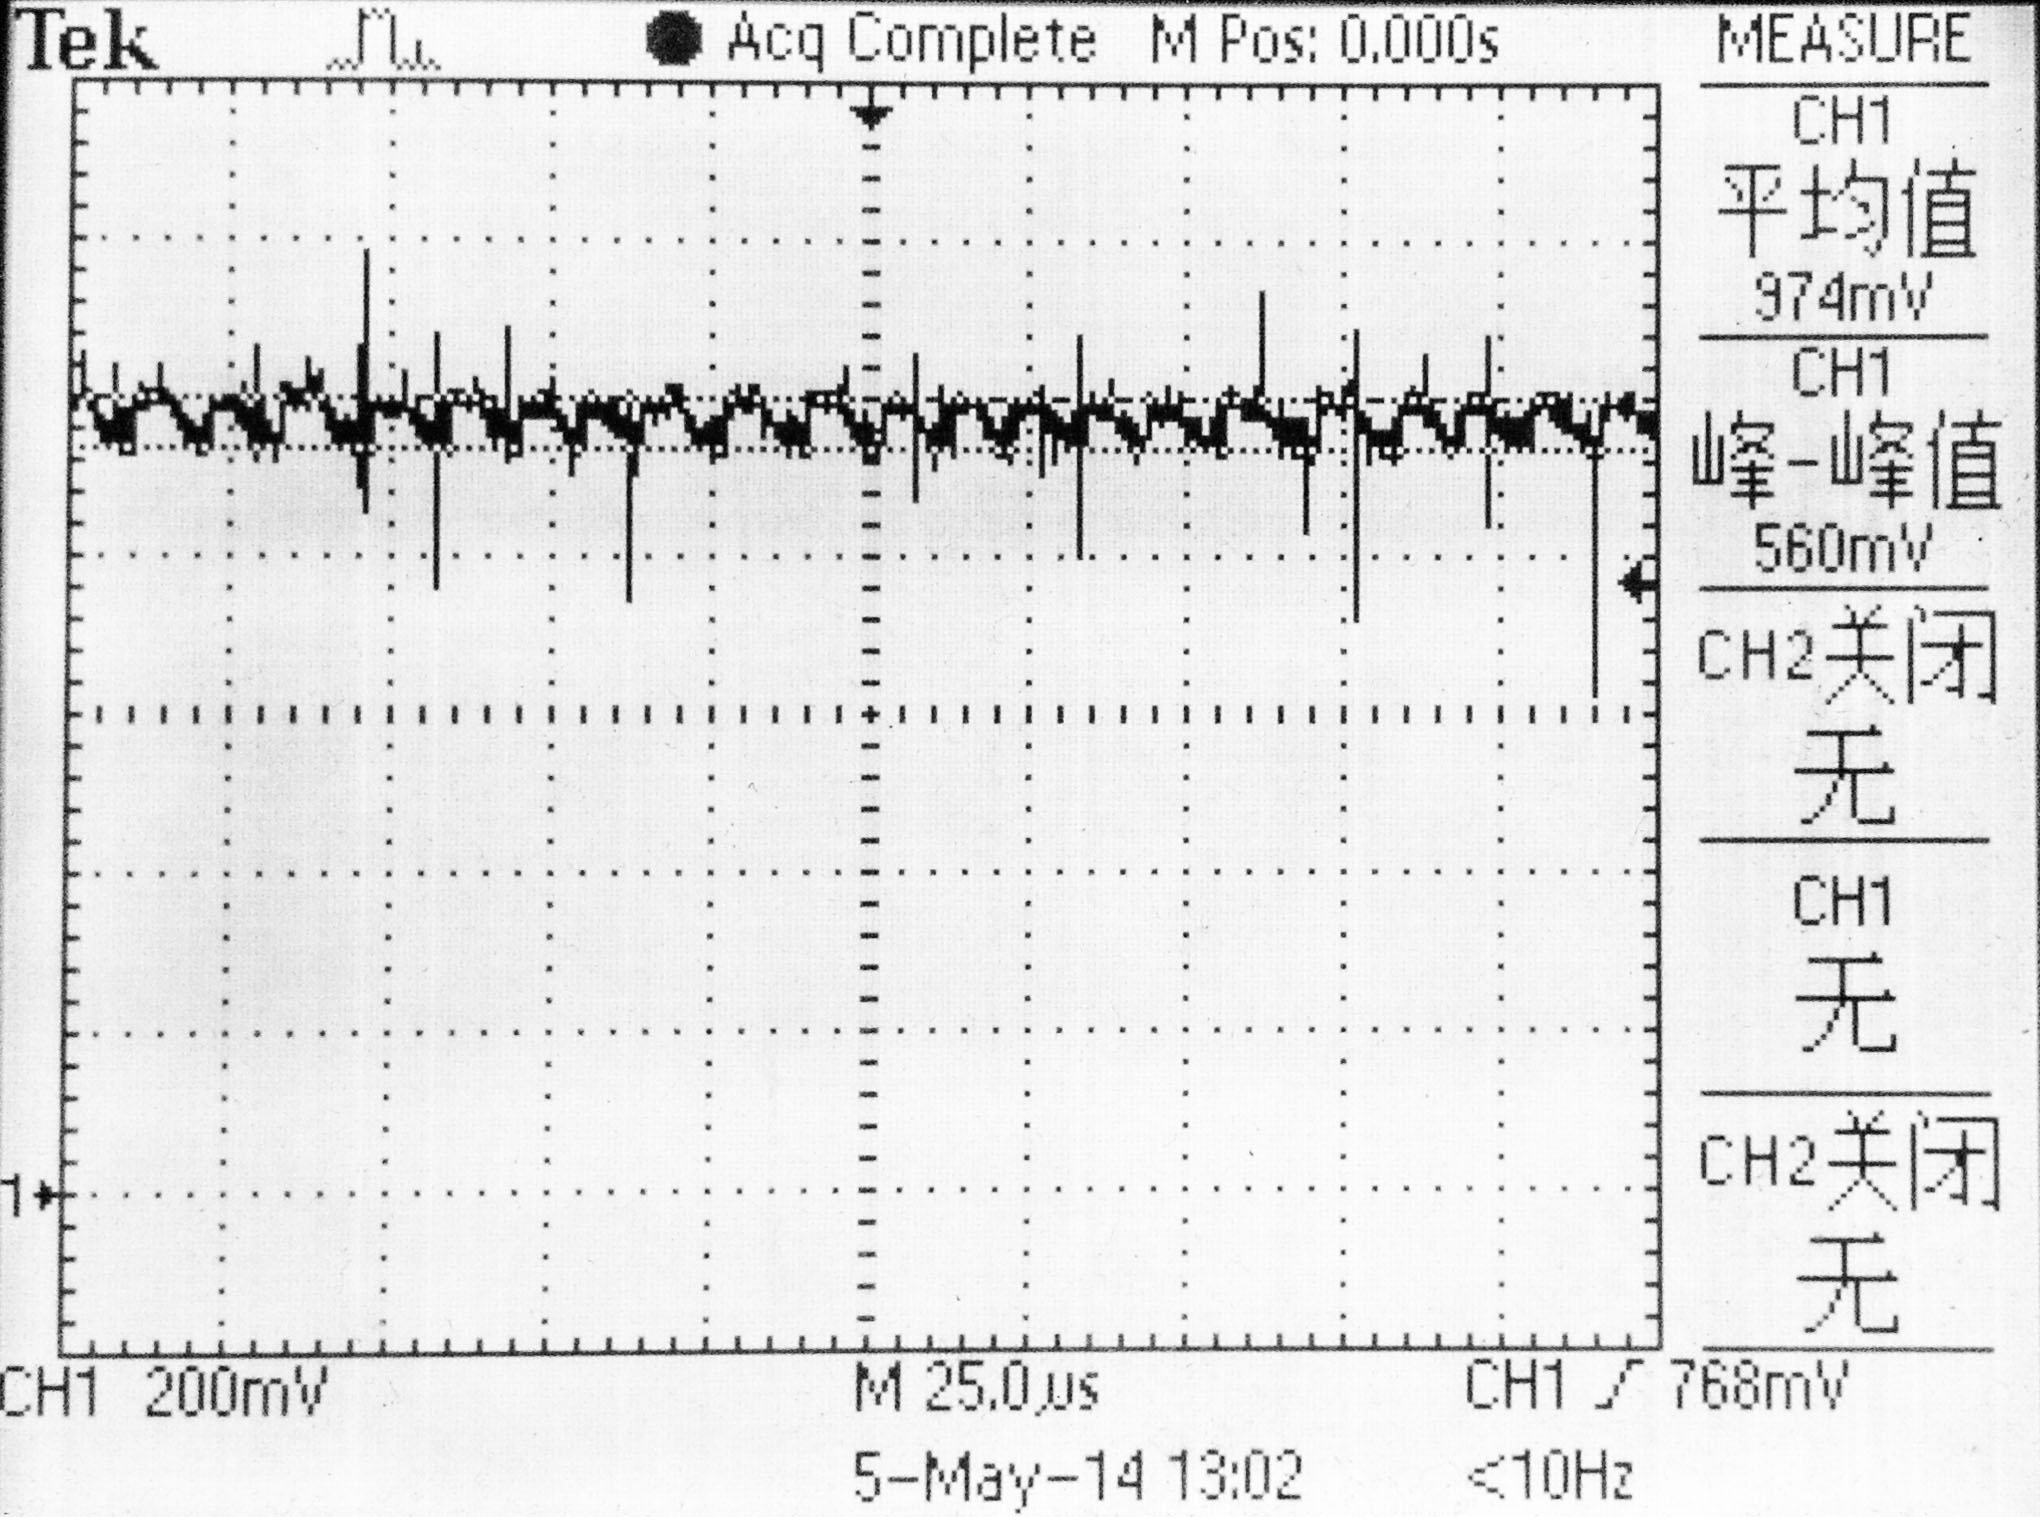
\includegraphics[height=0.45\textheight]{impl/pcb__pressure__emi__before.jpg}
    \caption{v0.2.1 无电源滤波}
    \label{fig:impl-pcb-pressure-emi-before}
  \end{subfigure}
  \par\bigskip
  \begin{subfigure}{1\textwidth}
    \centering
    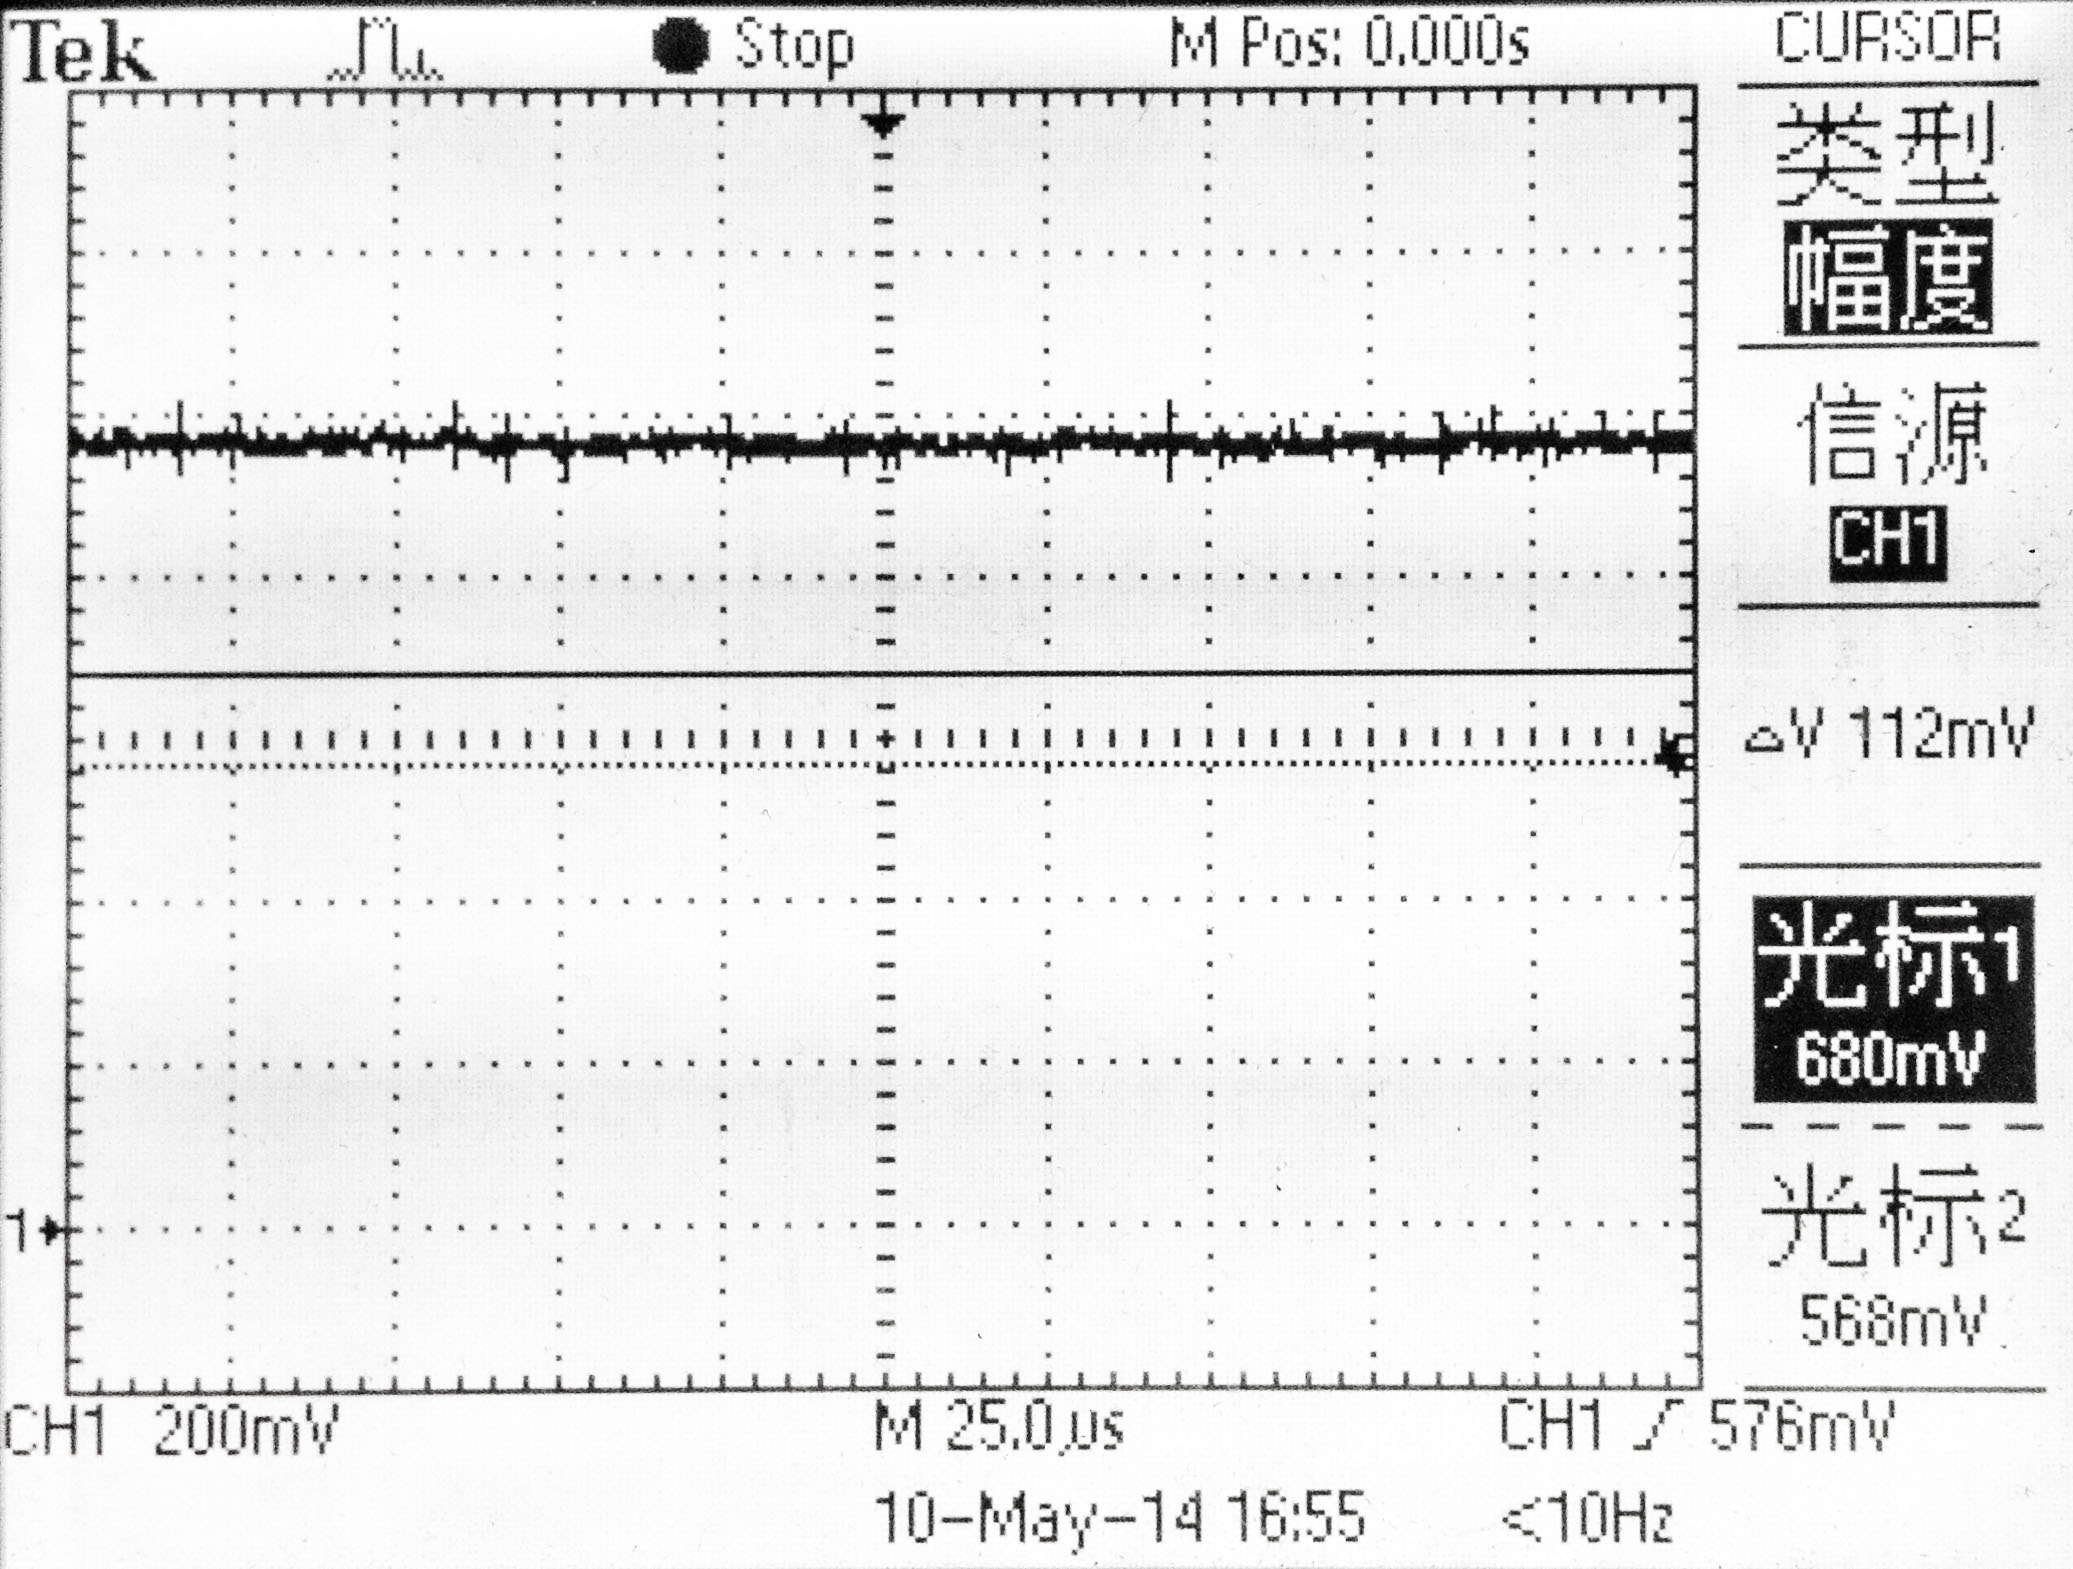
\includegraphics[height=0.45\textheight]{impl/pcb__pressure__emi__after.jpg}
    \caption{v0.3.1 有电源滤波}
    \label{fig:impl-pcb-pressure-emi-after}
  \end{subfigure}
\caption{背吹控制系统接口\csep 噪声比较}
\label{fig:impl-pcb-pressure-emi}
\end{figure}

\begin{sidewaysfigure}[p]
\centering
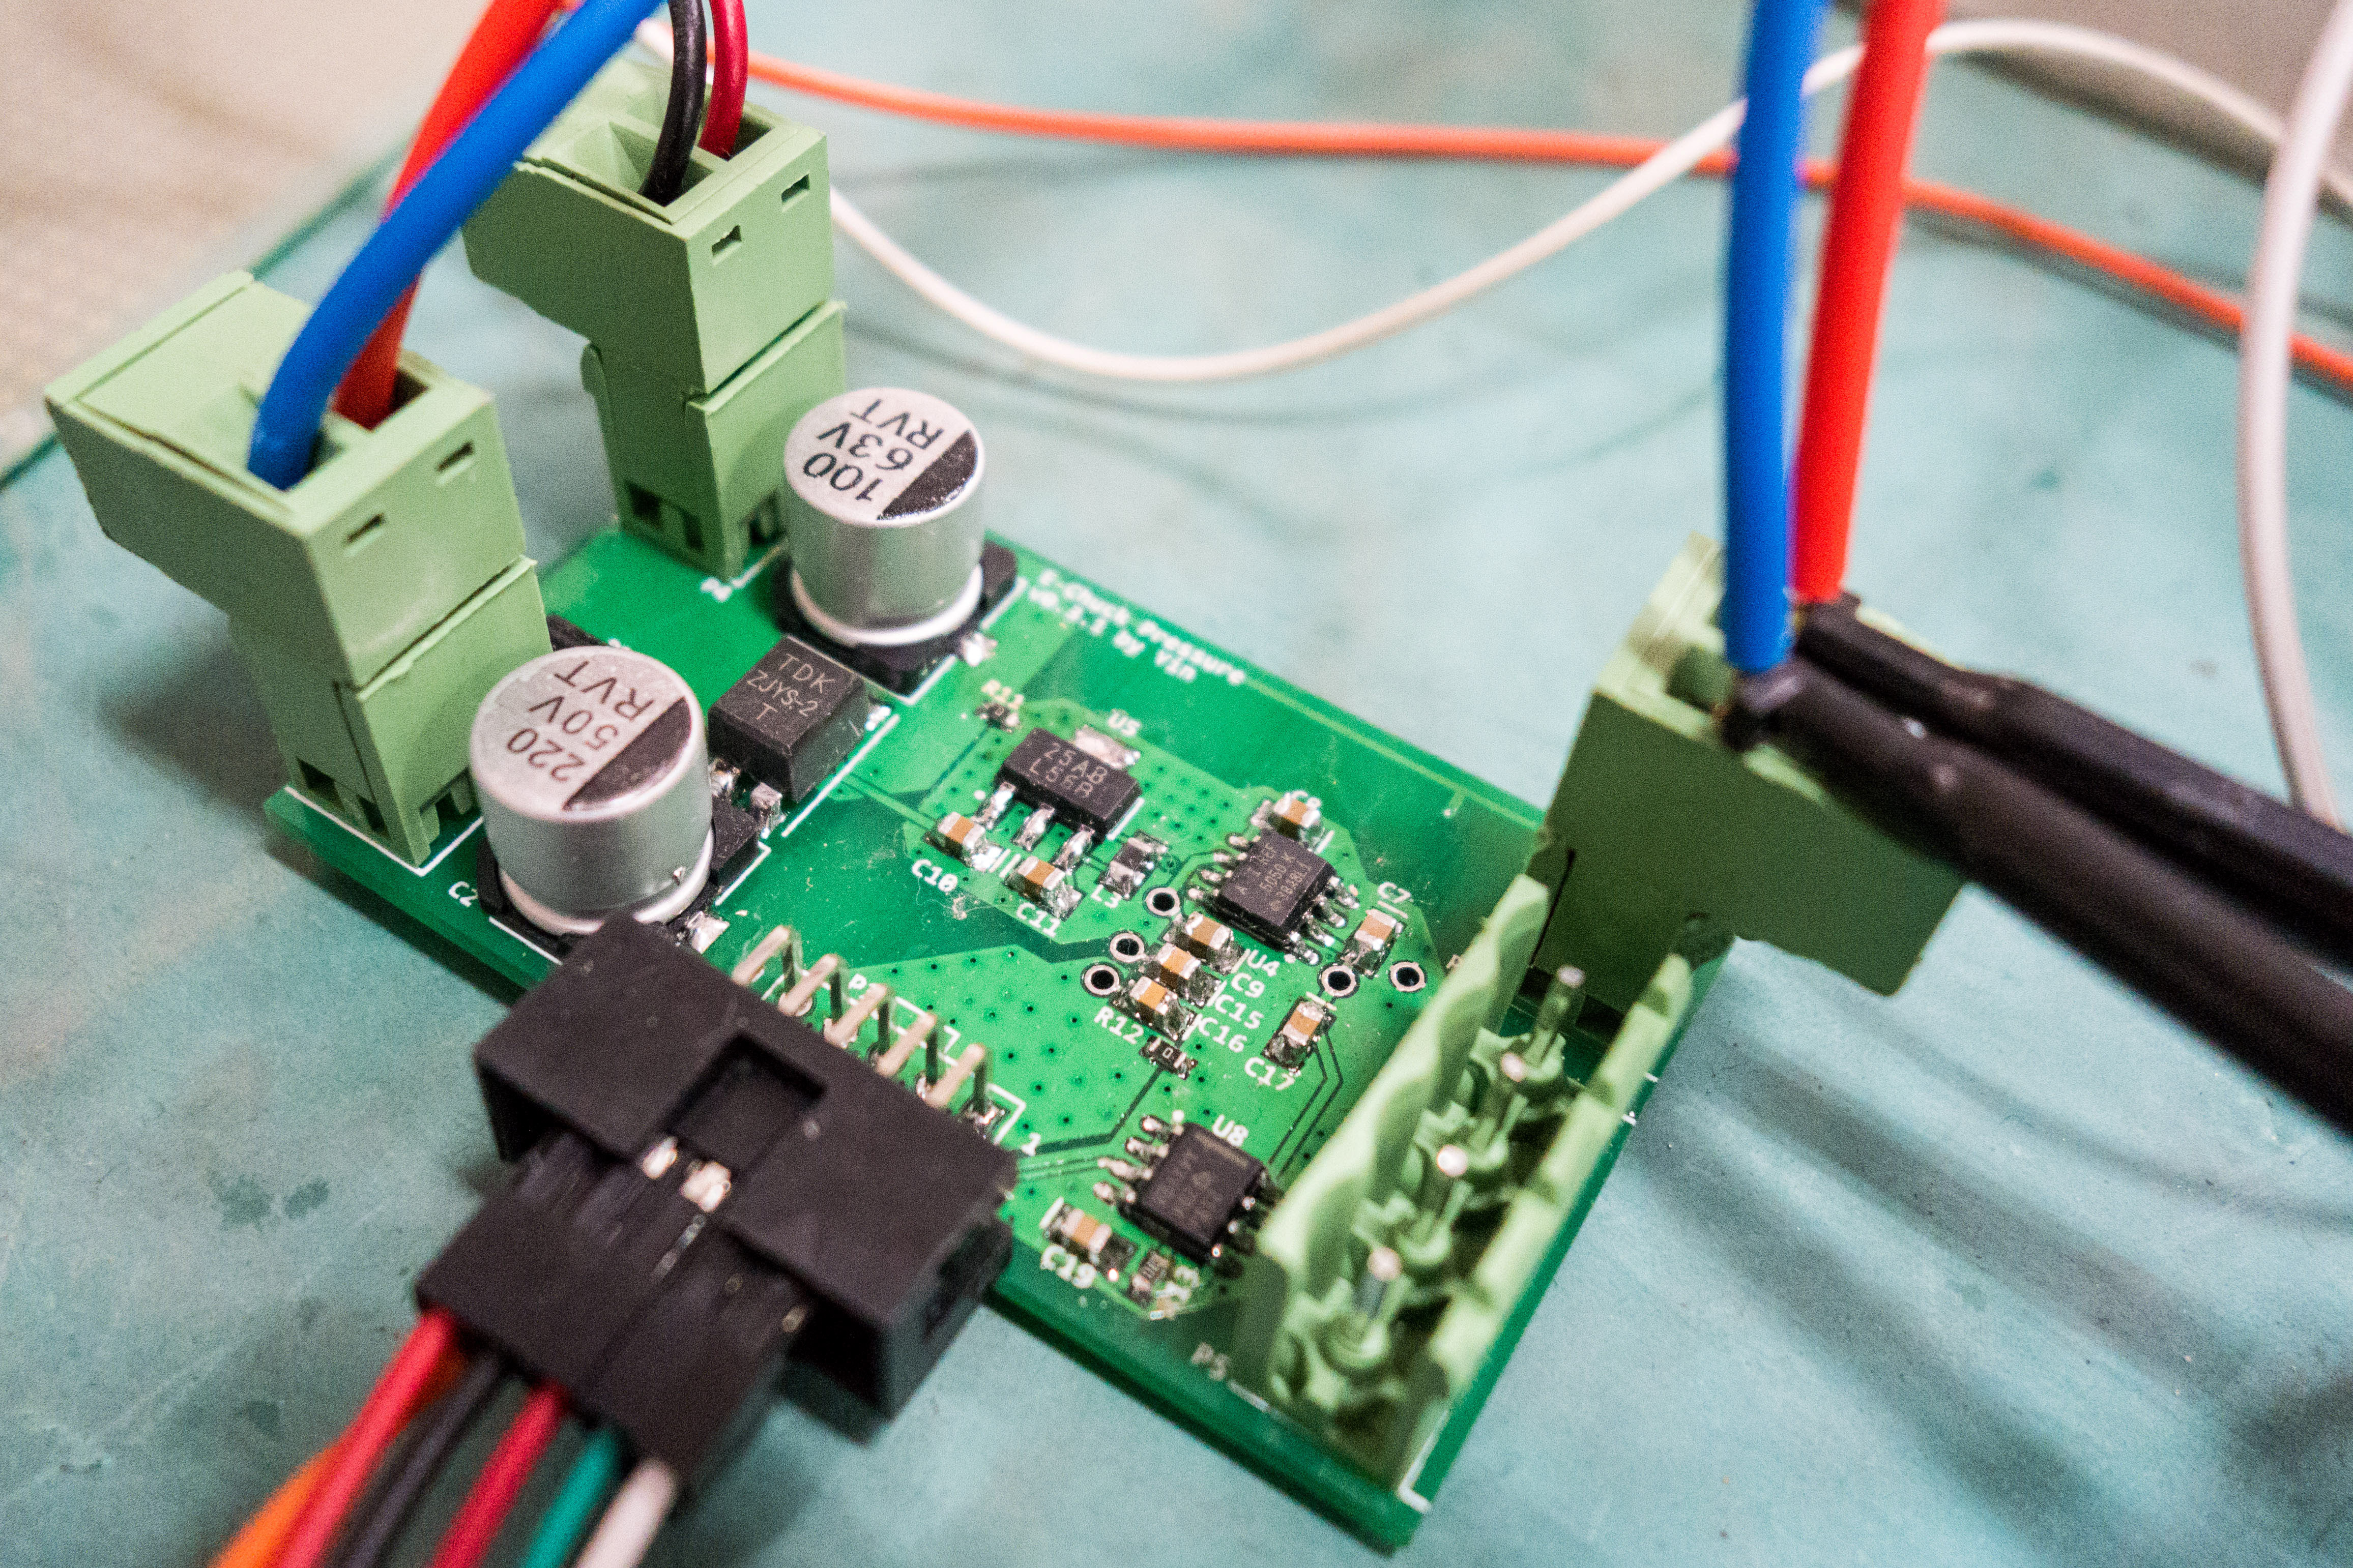
\includegraphics
  [max size={\textwidth}{0.9\textheight}]
  {impl/pcb__pressure__photo__pcb.jpg}
\caption{背吹控制系统接口\csep PCB}
\label{fig:impl-pcb-pressure-photo-pcb}
\end{sidewaysfigure}


\clearpage


\subsection{微力传感器接口}\label{sec:impl-pcb-ad7730}

\ref{sec:rig-ctrl-intf-strain}节中以AD7730为核心设计了微力传感器接口电路,本节将其实现为独立的PCB。根据图~\ref{fig:rig-ctrl-ad7730-ac}绘制完整的电路原理图(图~\ref{fig:impl-pcb-ad7730-sch})。电桥的激励端\bverb|E+|、\bverb|E-|与AD7730的参考输入接在一起,并可通过\bverb|J1|、\bverb|J2|跳线选择使用直流或交流激励:跳线2、3脚短接时,\bverb|E+|、\bverb|E-|分别接\SI{+5}{\V}与\SI{0}{\V},为直流激励;跳线1、2脚短接,并配置AD7730为交流激励模式后,AD7730输出\bverb|ACX|换向信号至DRV8837集成H桥芯片,向电桥施加交流激励,AD7730可自动处理正、反相信号,并补偿信号传输与开关延迟。\bverb|P1|接微力传感器(电桥),选用标准可插拔式接线端子;\bverb|P2|接MCU(数据、供电),选用标准10针简单牛角接头。

在制作PCB前,先在万用板上使用直插封装的AD7730制作了直流激励部分的电路,并使用已有的电桥传感器,接入MCU进行原理验证测试,确认了其功能一切正常;然后将LSB200微力传感器接入万用板进行测试,如图~\ref{fig:impl-pcb-ad7730-photo-perf},功能一切正常;最后,制作并焊接PCB,如图~\ref{fig:impl-pcb-ad7730-photo-pcb},实测总有效分辨率(包含传感器自身噪声在内)约为\SI{14}{\bit},完全满足性能要求。

\begin{figure}[tbhp]
\centering
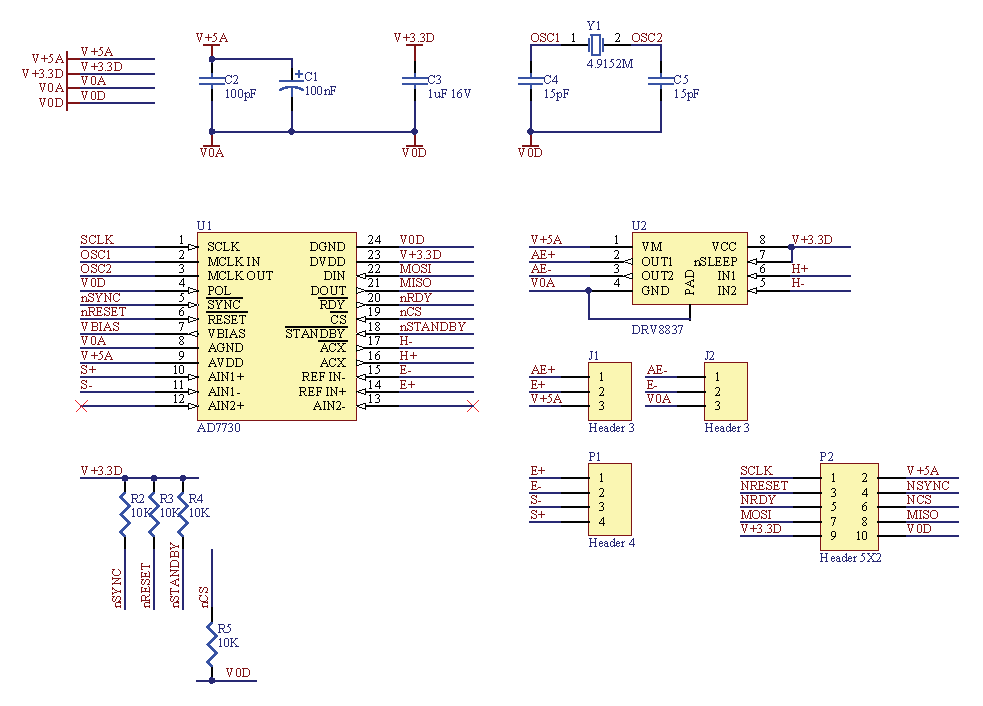
\includegraphics[width=1\linewidth]{impl/pcb__ad7730__sch}
\caption{AD7730电桥接口\csep 原理图}
\label{fig:impl-pcb-ad7730-sch}
\end{figure}

\begin{figure}[tbhp]
\centering
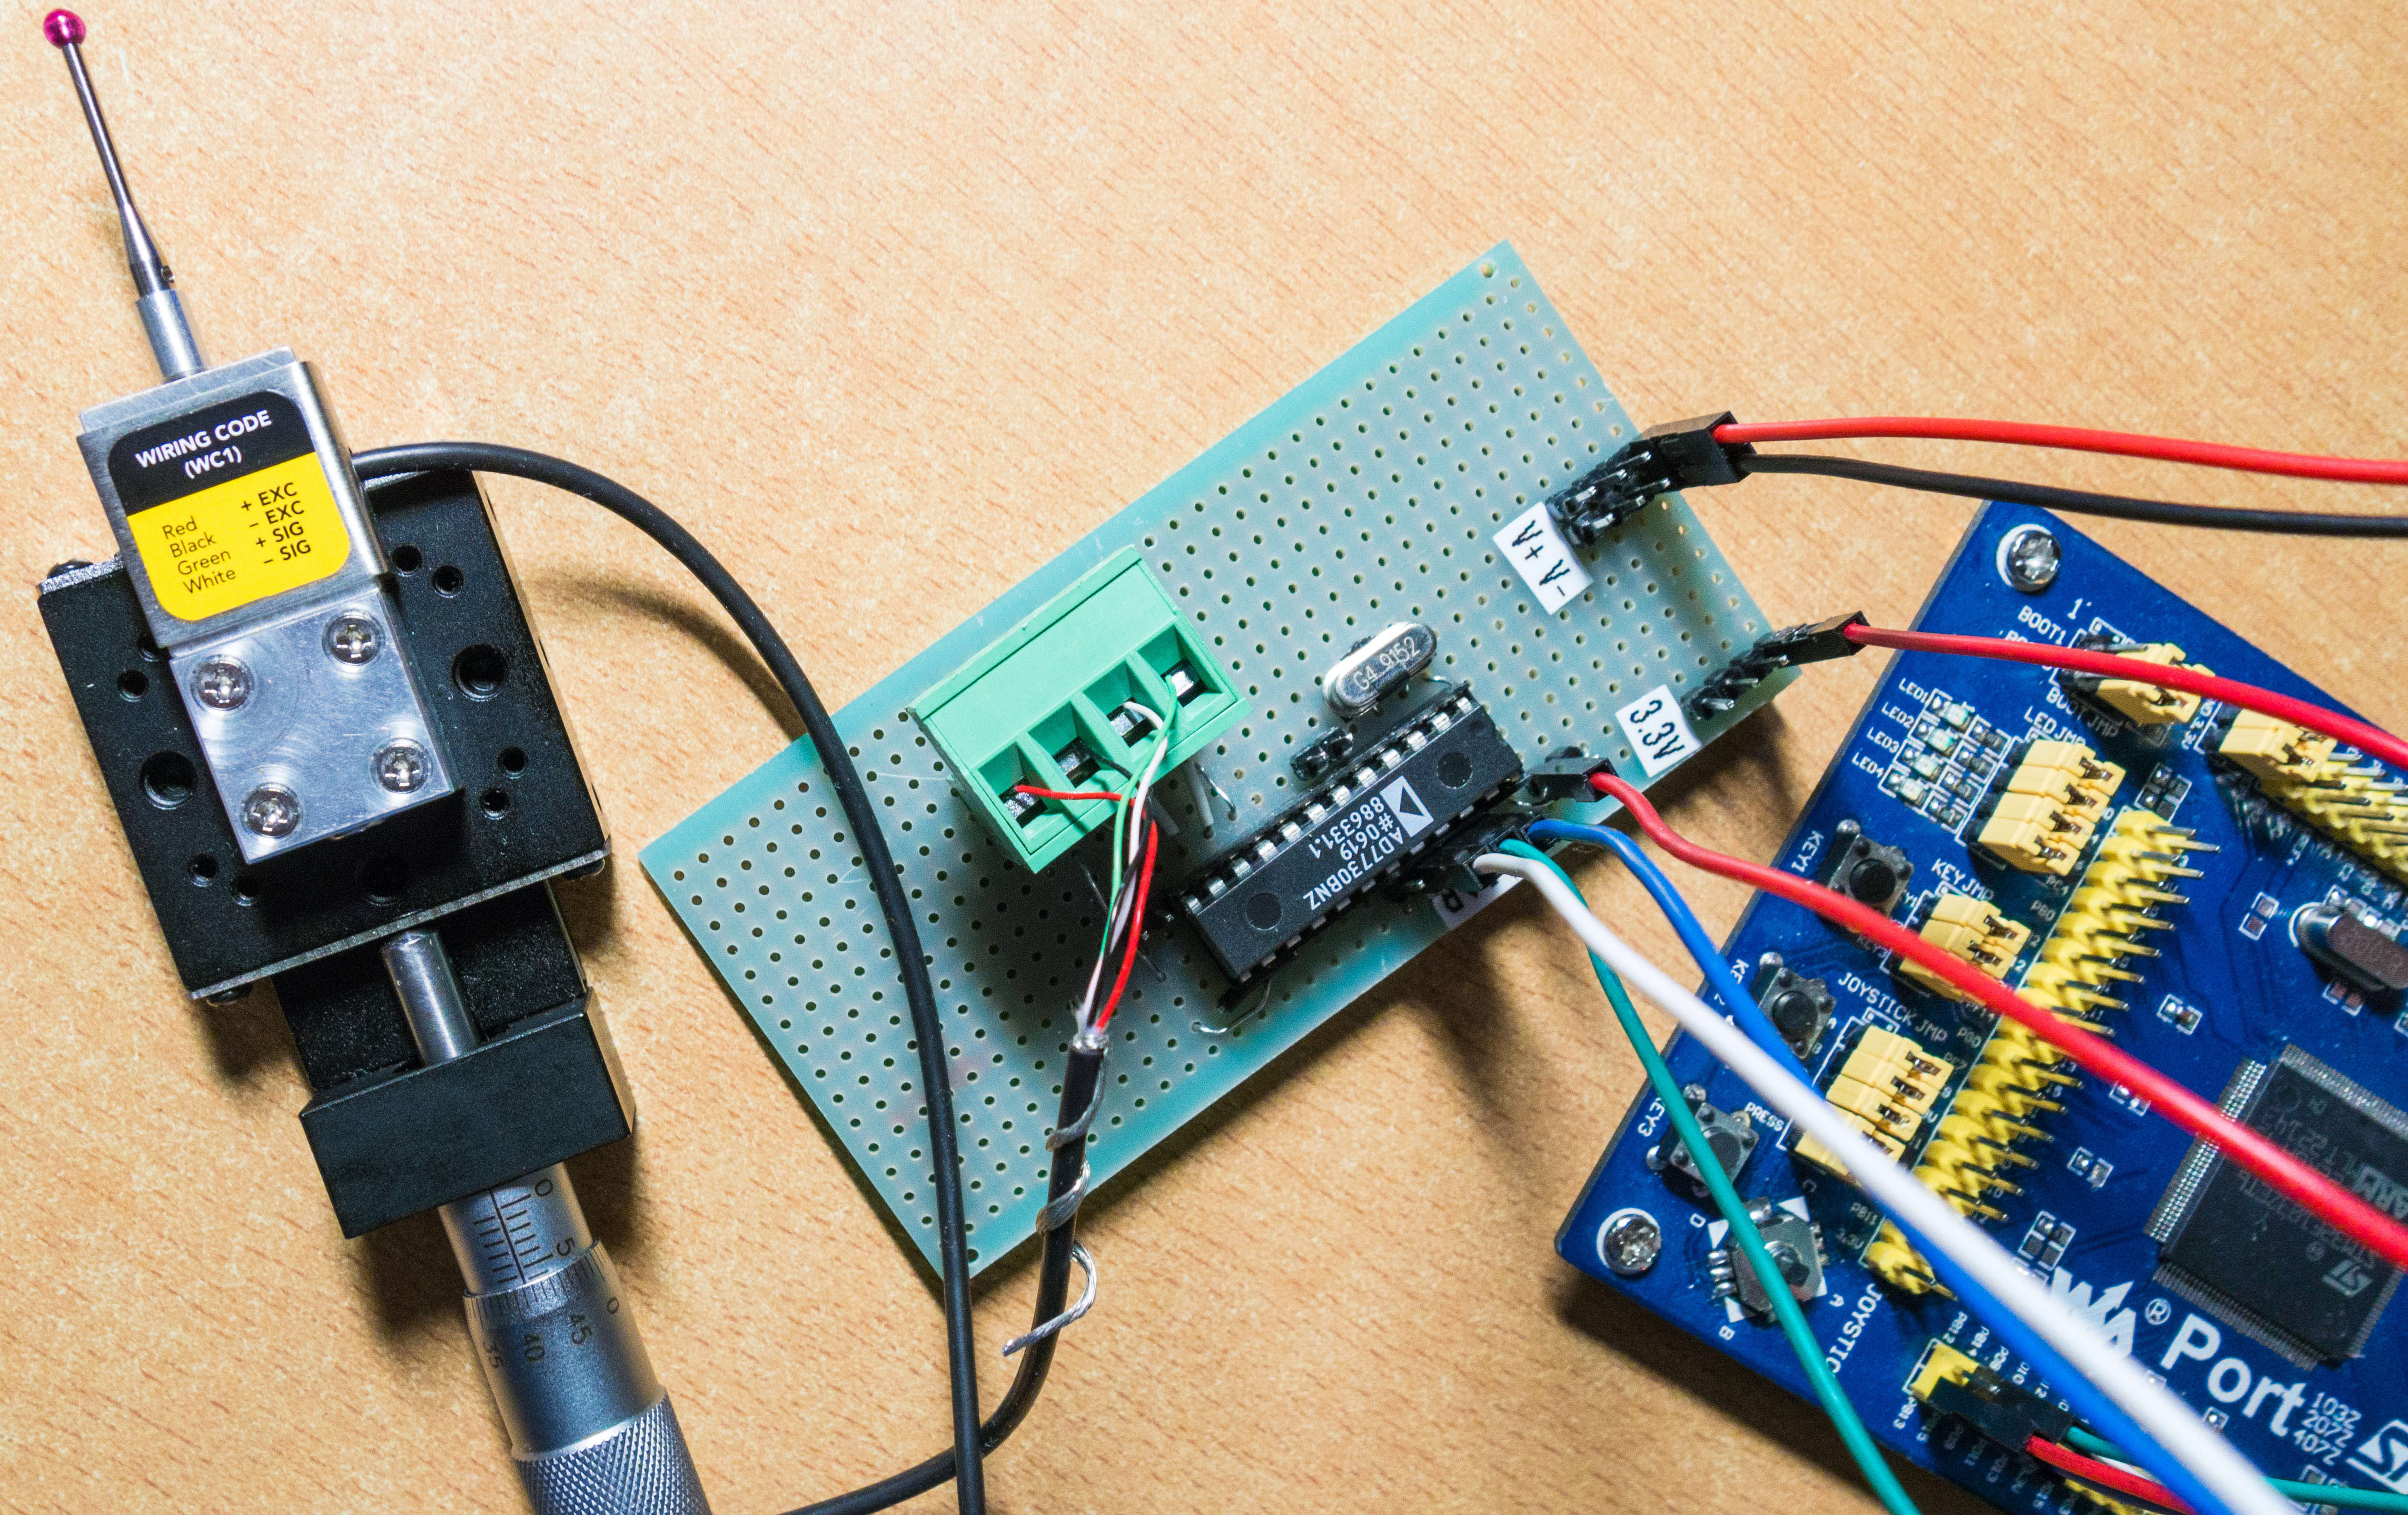
\includegraphics[width=0.8\linewidth]{impl/pcb__ad7730__photo__perf.jpg}
\caption{AD7730电桥接口\csep 万用板测试}
\label{fig:impl-pcb-ad7730-photo-perf}
\end{figure}

\begin{figure}[tbhp]
\centering
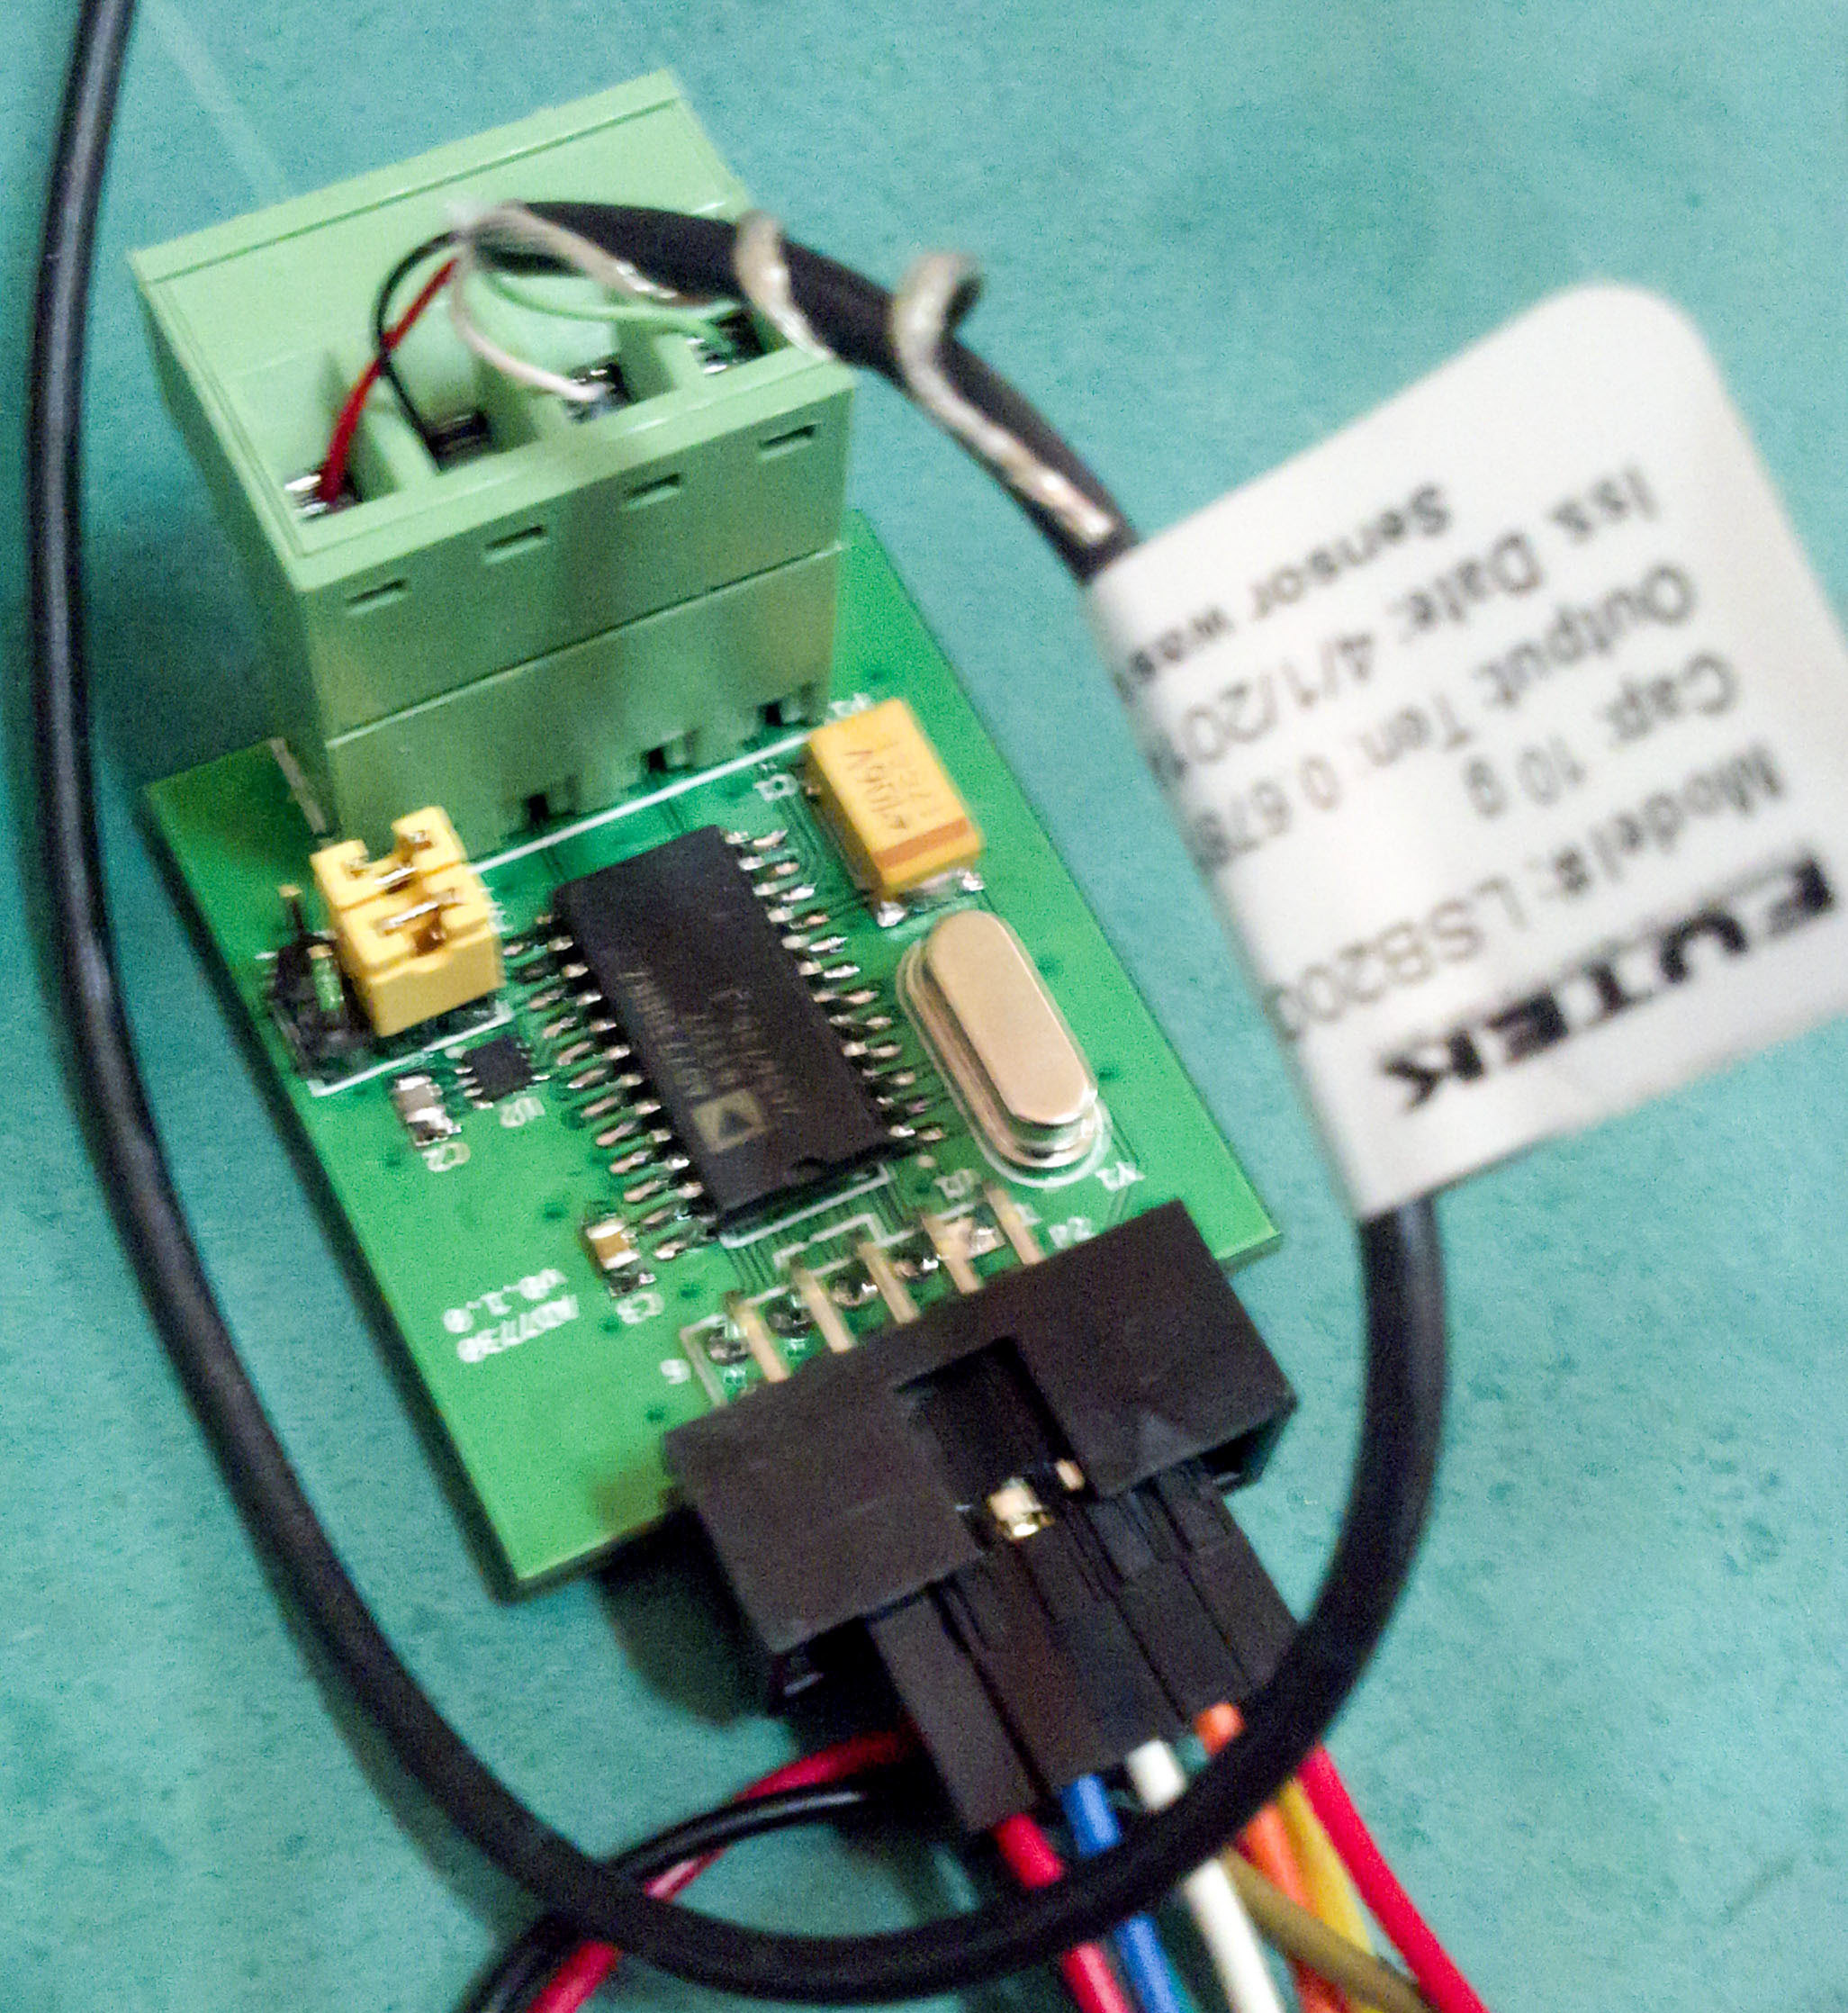
\includegraphics[height=0.45\textheight]{impl/pcb__ad7730__photo__pcb.jpg}
\caption{AD7730电桥接口\csep PCB}
\label{fig:impl-pcb-ad7730-photo-pcb}
\end{figure}


\clearpage


\subsection{LAC-10A电动推杆接口}\label{sec:impl-pcb-zaber}

\ref{sec:rig-ctrl-intf-stepper}节中讨论了LAC-10A内置步进电机的驱动器选型以及零位传感器部分的设计。以下讨论这两部分的具体实现。

\subsubsection{步进电机驱动}\label{sec:impl-pcb-zaber-stepper}

选配的DM422C型驱动器如图~\ref{fig:impl-pcb-zaber-dm422c}:使用\SI{+24}{\V}为其供电,通过MAX490差分输入输出芯片(用万用板实现,如图~\ref{fig:impl-pcb-zaber-max490})从MCU接收方向/脉冲控制信号。

\begin{figure}[tbh]
\centering
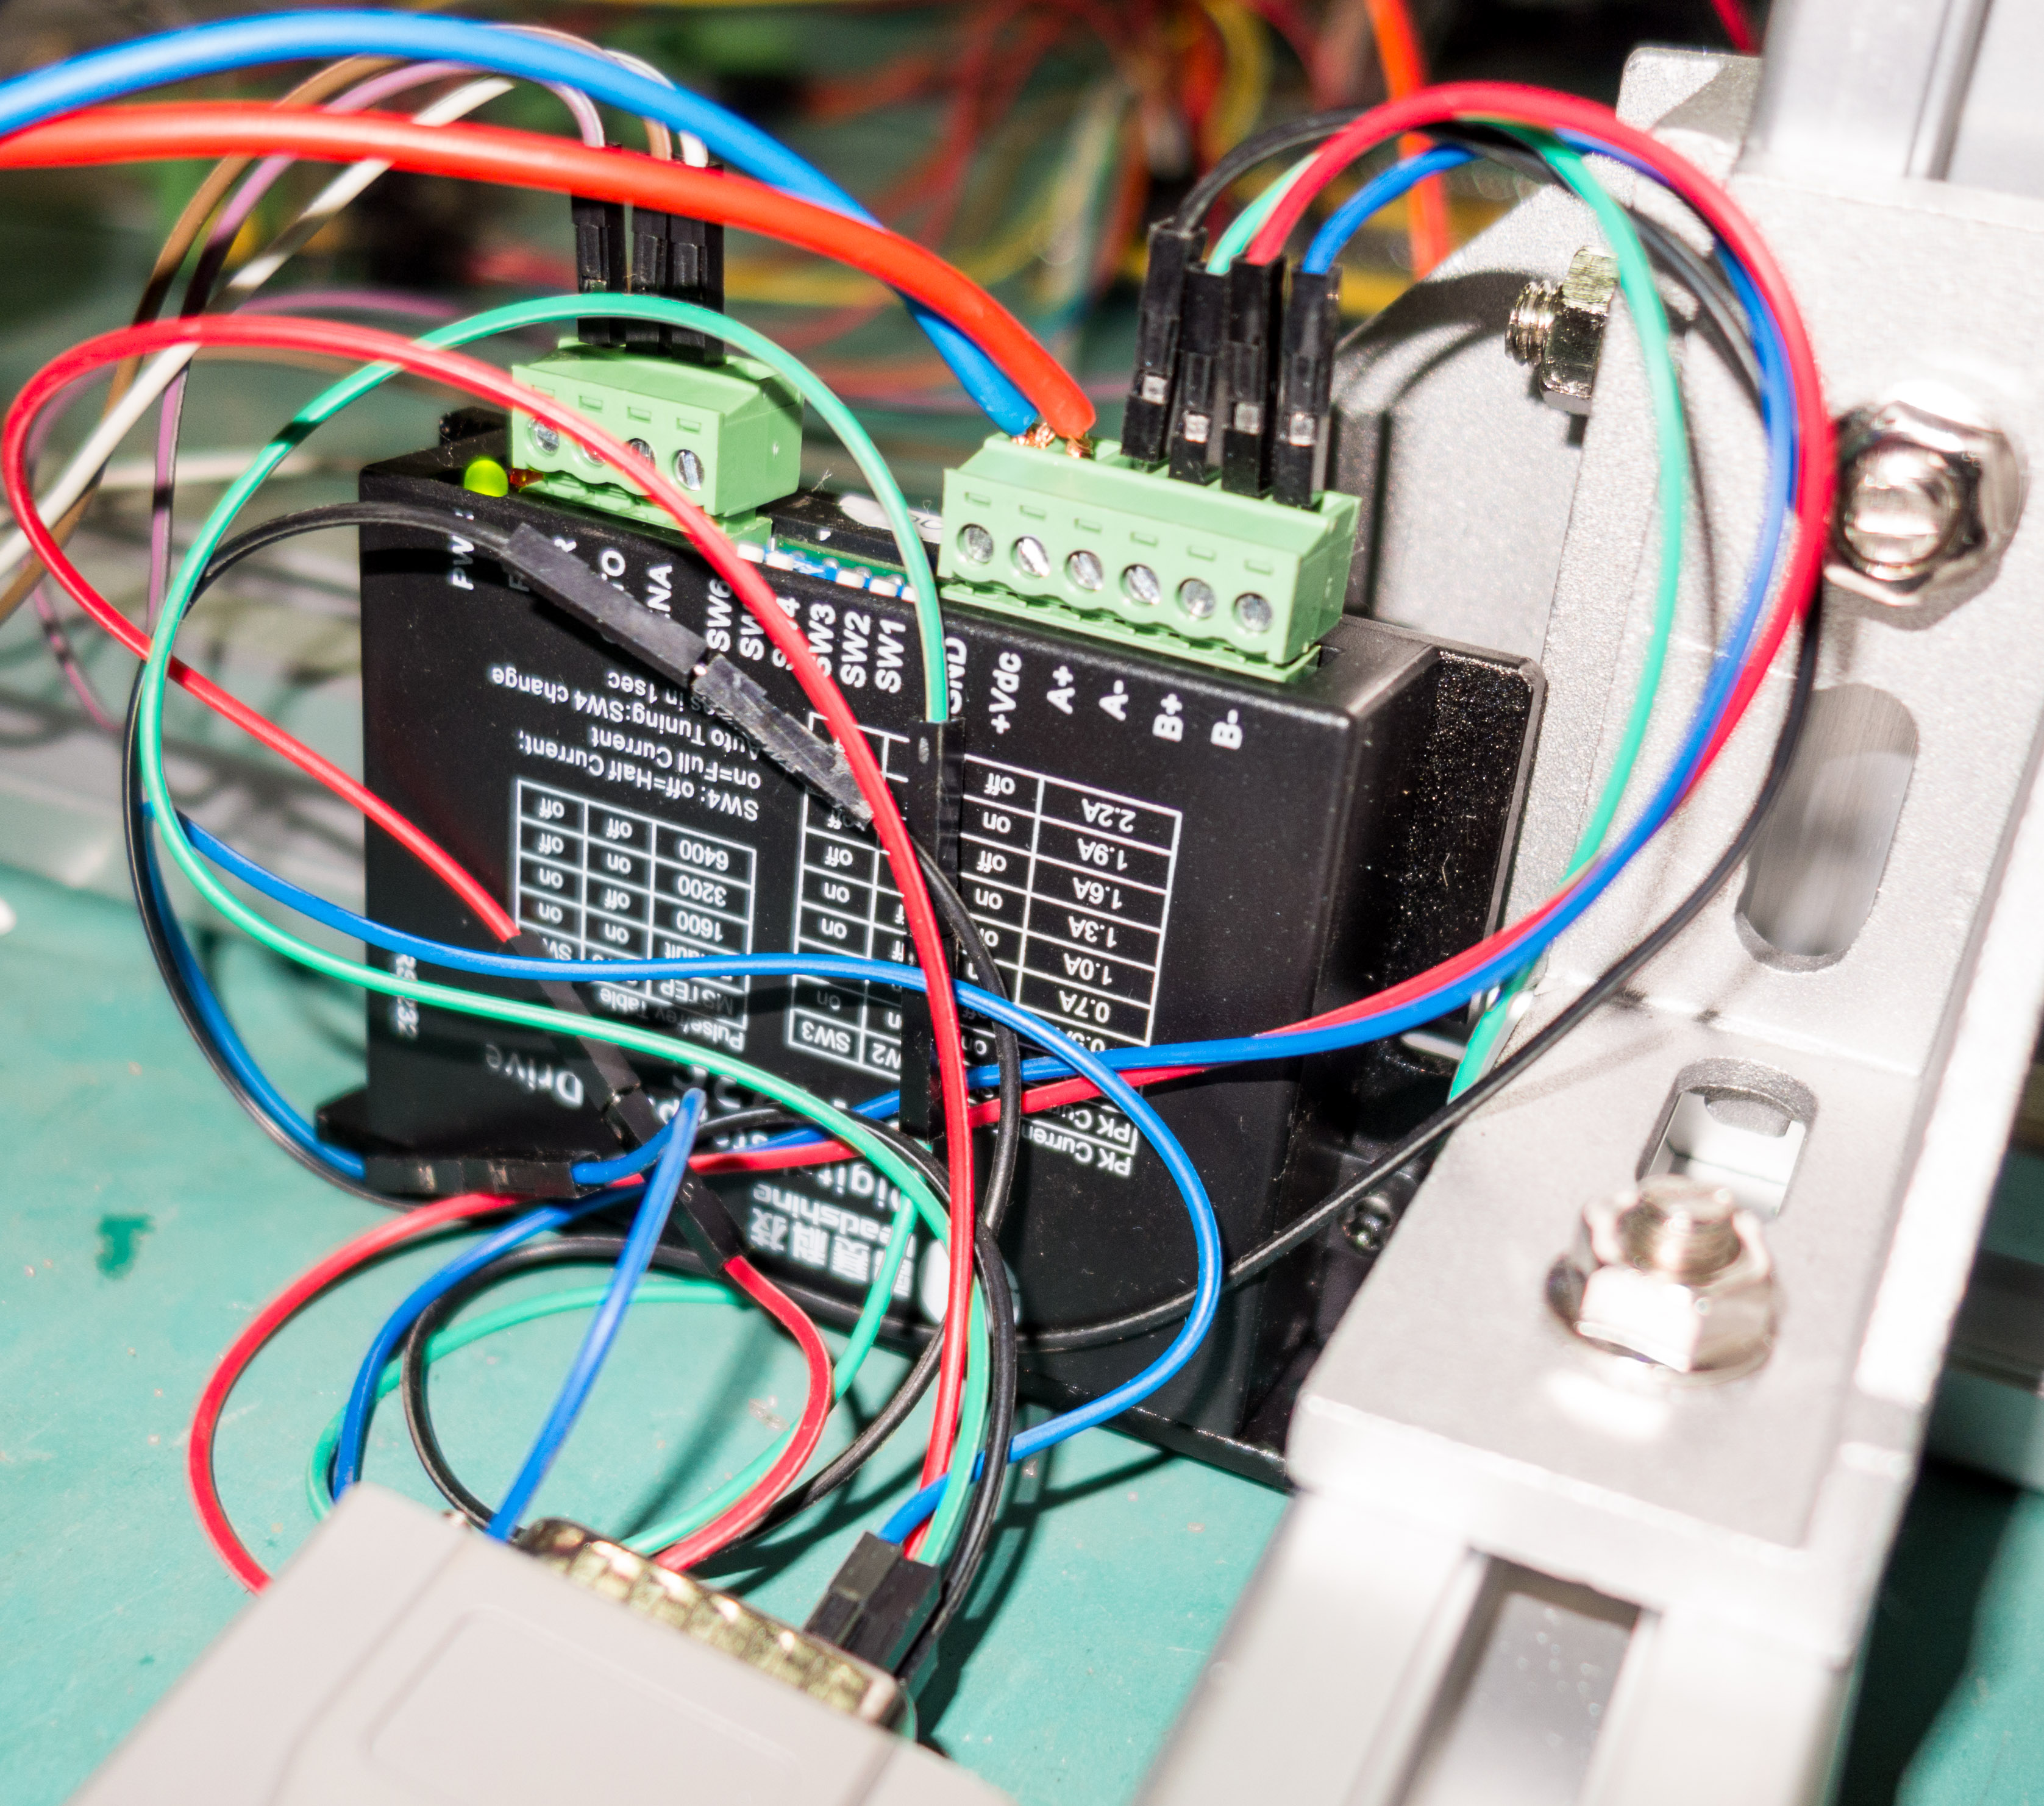
\includegraphics[width=0.55\linewidth]{impl/pcb__zaber__dm422c.jpg}
\caption{DM422C步进电机驱动器实物图}
\label{fig:impl-pcb-zaber-dm422c}
\end{figure}

\begin{figure}[tbh]
\centering
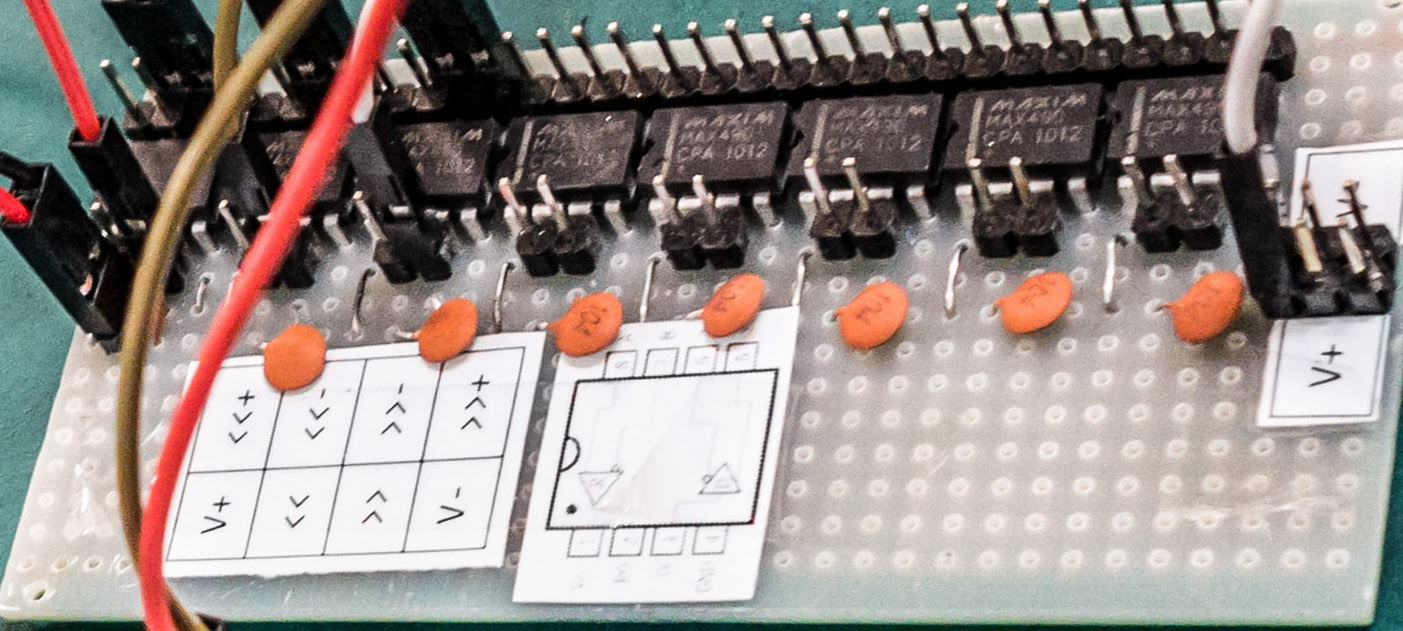
\includegraphics[width=0.55\linewidth]{impl/pcb__zaber__max490.jpg}
\caption{MAX490差分输入输出板实物图}
\label{fig:impl-pcb-zaber-max490}
\end{figure}

\subsubsection{零位传感器及接口}\label{sec:impl-pcb-zaber-homing}

为零位传感器设计的光耦隔离接口电路原理参见图~\ref{fig:rig-ctrl-intf-opto}。由于其组成简单,直接用万用板与直插封装光耦制作,如图~\ref{fig:impl-pcb-zaber-opto-perf}:白色IC为光耦,色环电阻为光耦输入端限流电阻,右侧棕色的线表示直接焊在万用板上的贴片上拉电阻。虽然使用该电路可减小误触发概率,但实测发现一个问题:当步进电机运行时,由于LAC-10A的零位传感器信号线与其步进电机接线处于同一电缆中,且无任何屏蔽措施,仅在步进电机处于上电保持状态时,其输出上的电磁干扰峰峰值($V_{\mathrm{pp}}$)就已超过\SI{8}{\V}(图~\ref{fig:impl-pcb-zaber-emi-before}),即使使用较高电压供电,也不能完全排除误触发现象。因此,为LAC-10A重新设计零位传感器,如图~\ref{fig:impl-pcb-zaber-new-sch}:采用同图~\ref{fig:impl-pcb-pressure-sch-power-filter}~类似的简易保护与滤波电路,并在传感器输出端加入滤波电容,以改善其抗干扰能力。由于需匹配电动推杆后部的安装尺寸,将该电路实现为PCB,安装后如图~\ref{fig:impl-pcb-zaber-new-photo}。上电实测发现电磁干扰得到有效控制,无误触发现象,与光耦接口电路配合可得到高质量的零位信号。

\begin{figure}[tbhp]
\centering
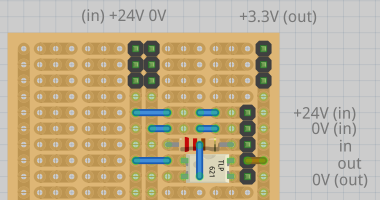
\includegraphics[width=0.618\linewidth]{impl/pcb__zaber__opto__perf.png}
\caption{LAC-10A零位传感器\csep 光耦接口\csep 万用板}
\label{fig:impl-pcb-zaber-opto-perf}
\end{figure}

\begin{figure}[tbhp]
\centering
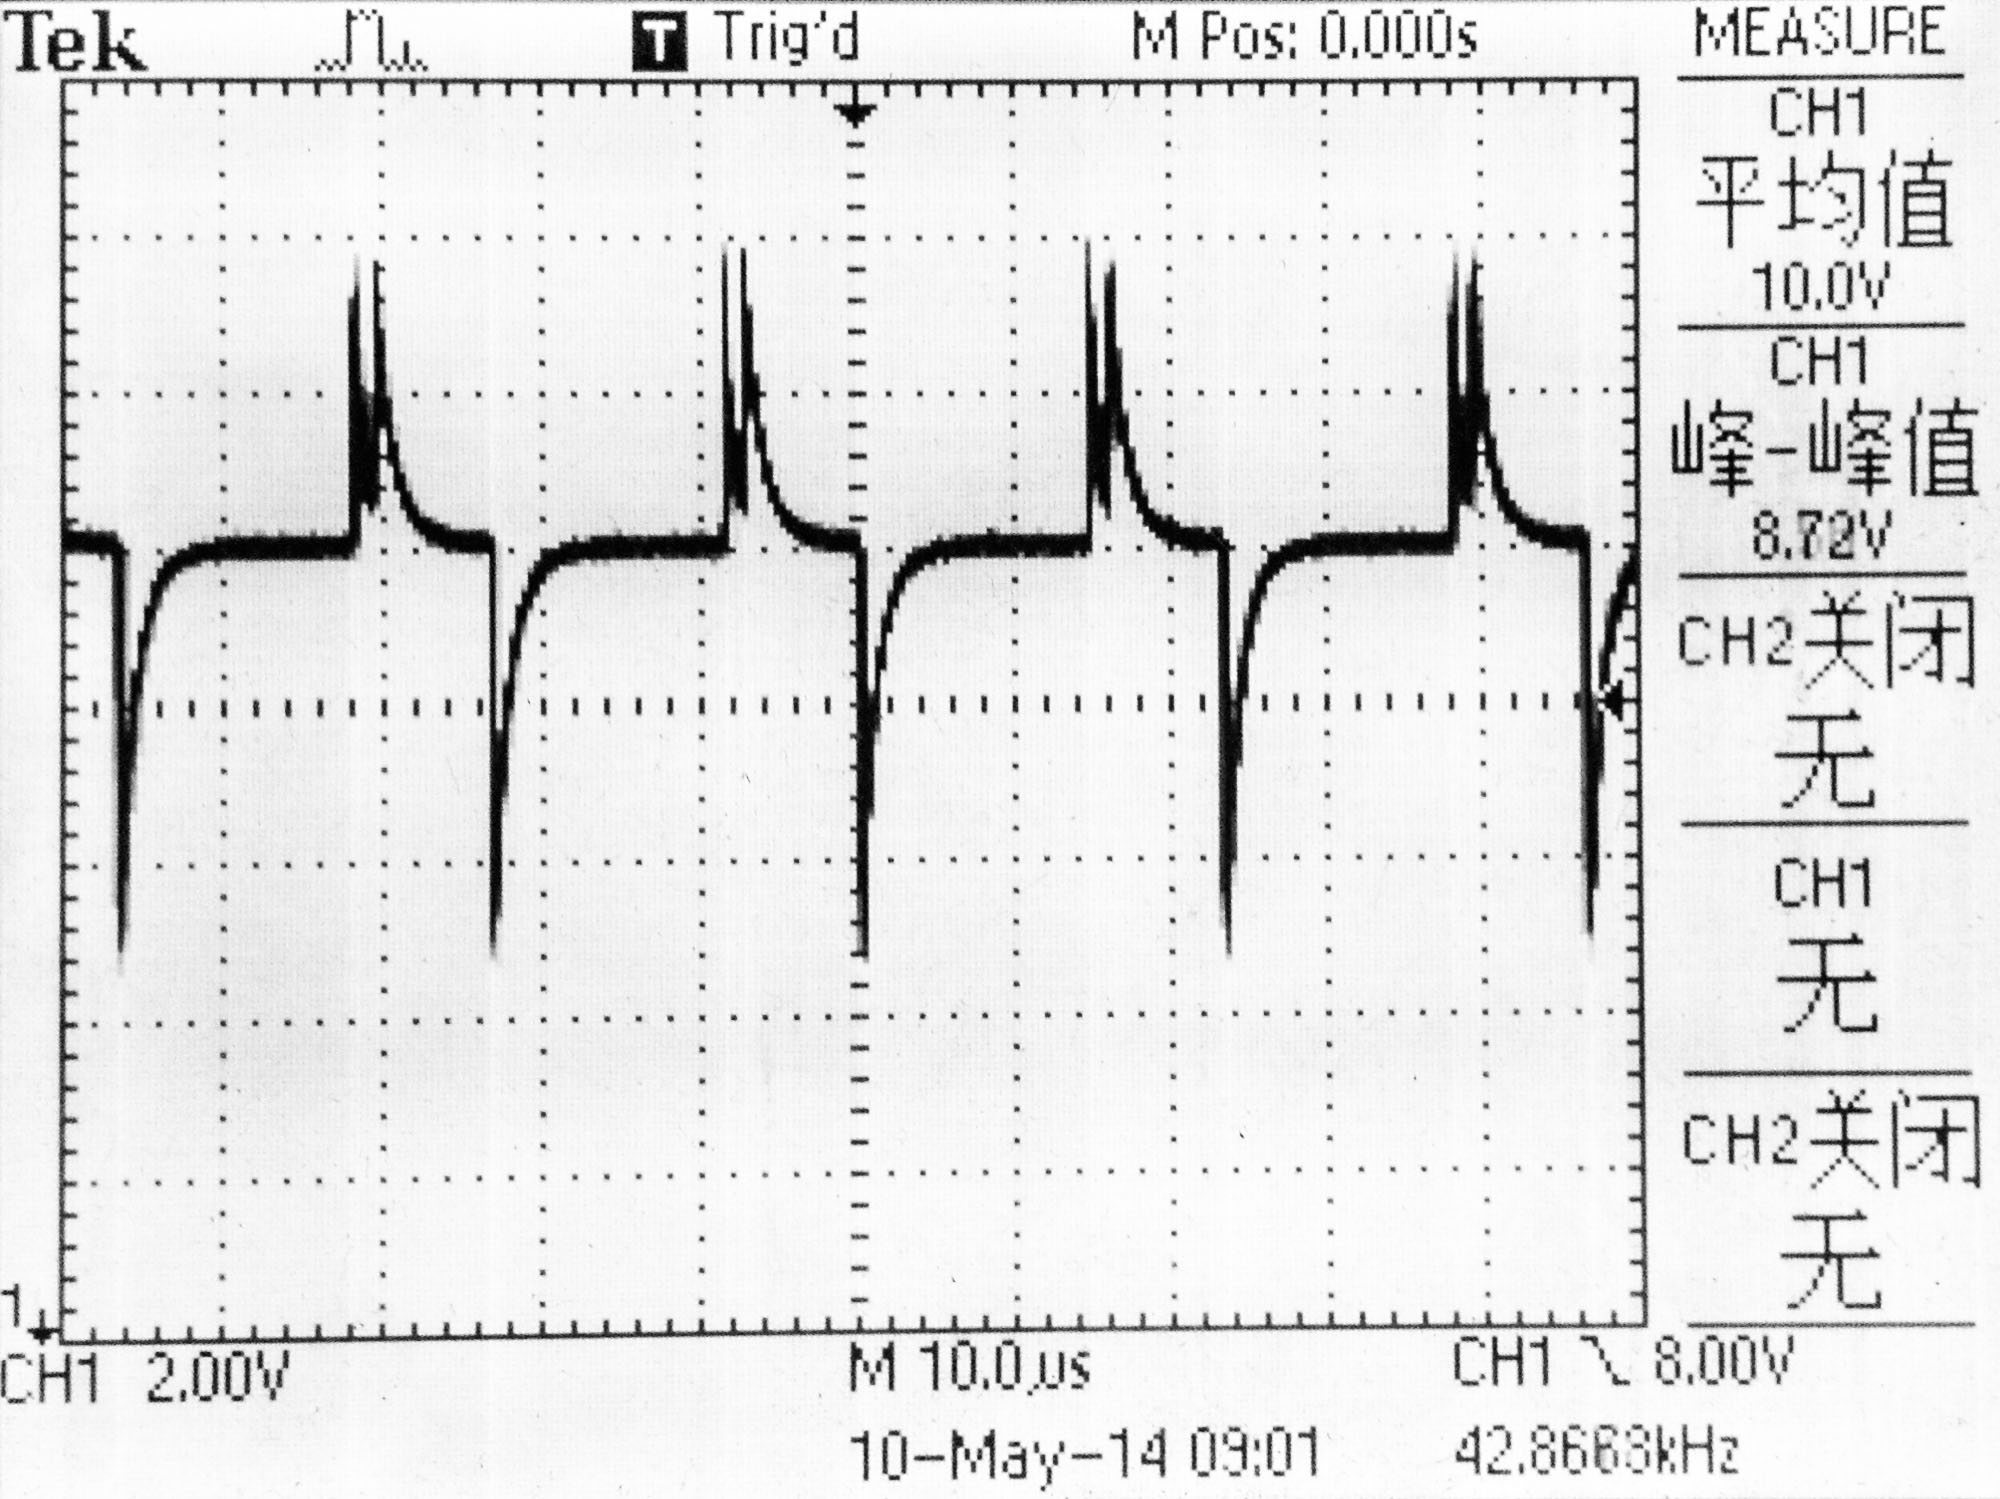
\includegraphics[height=0.32\textheight]{impl/pcb__zaber__emi__before.jpg}
\caption{LAC-10A零位传感器\csep 电磁干扰}
\label{fig:impl-pcb-zaber-emi-before}
\end{figure}

\begin{figure}[p]
\centering
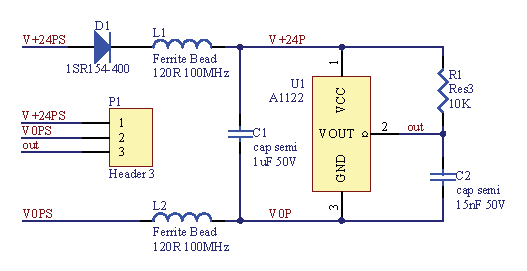
\includegraphics[width=0.80\linewidth]{impl/pcb__zaber__new__sch}
\caption{LAC-10A零位传感器\csep 新设计\csep 原理图}
\label{fig:impl-pcb-zaber-new-sch}
\end{figure}

\begin{figure}[p]
\centering
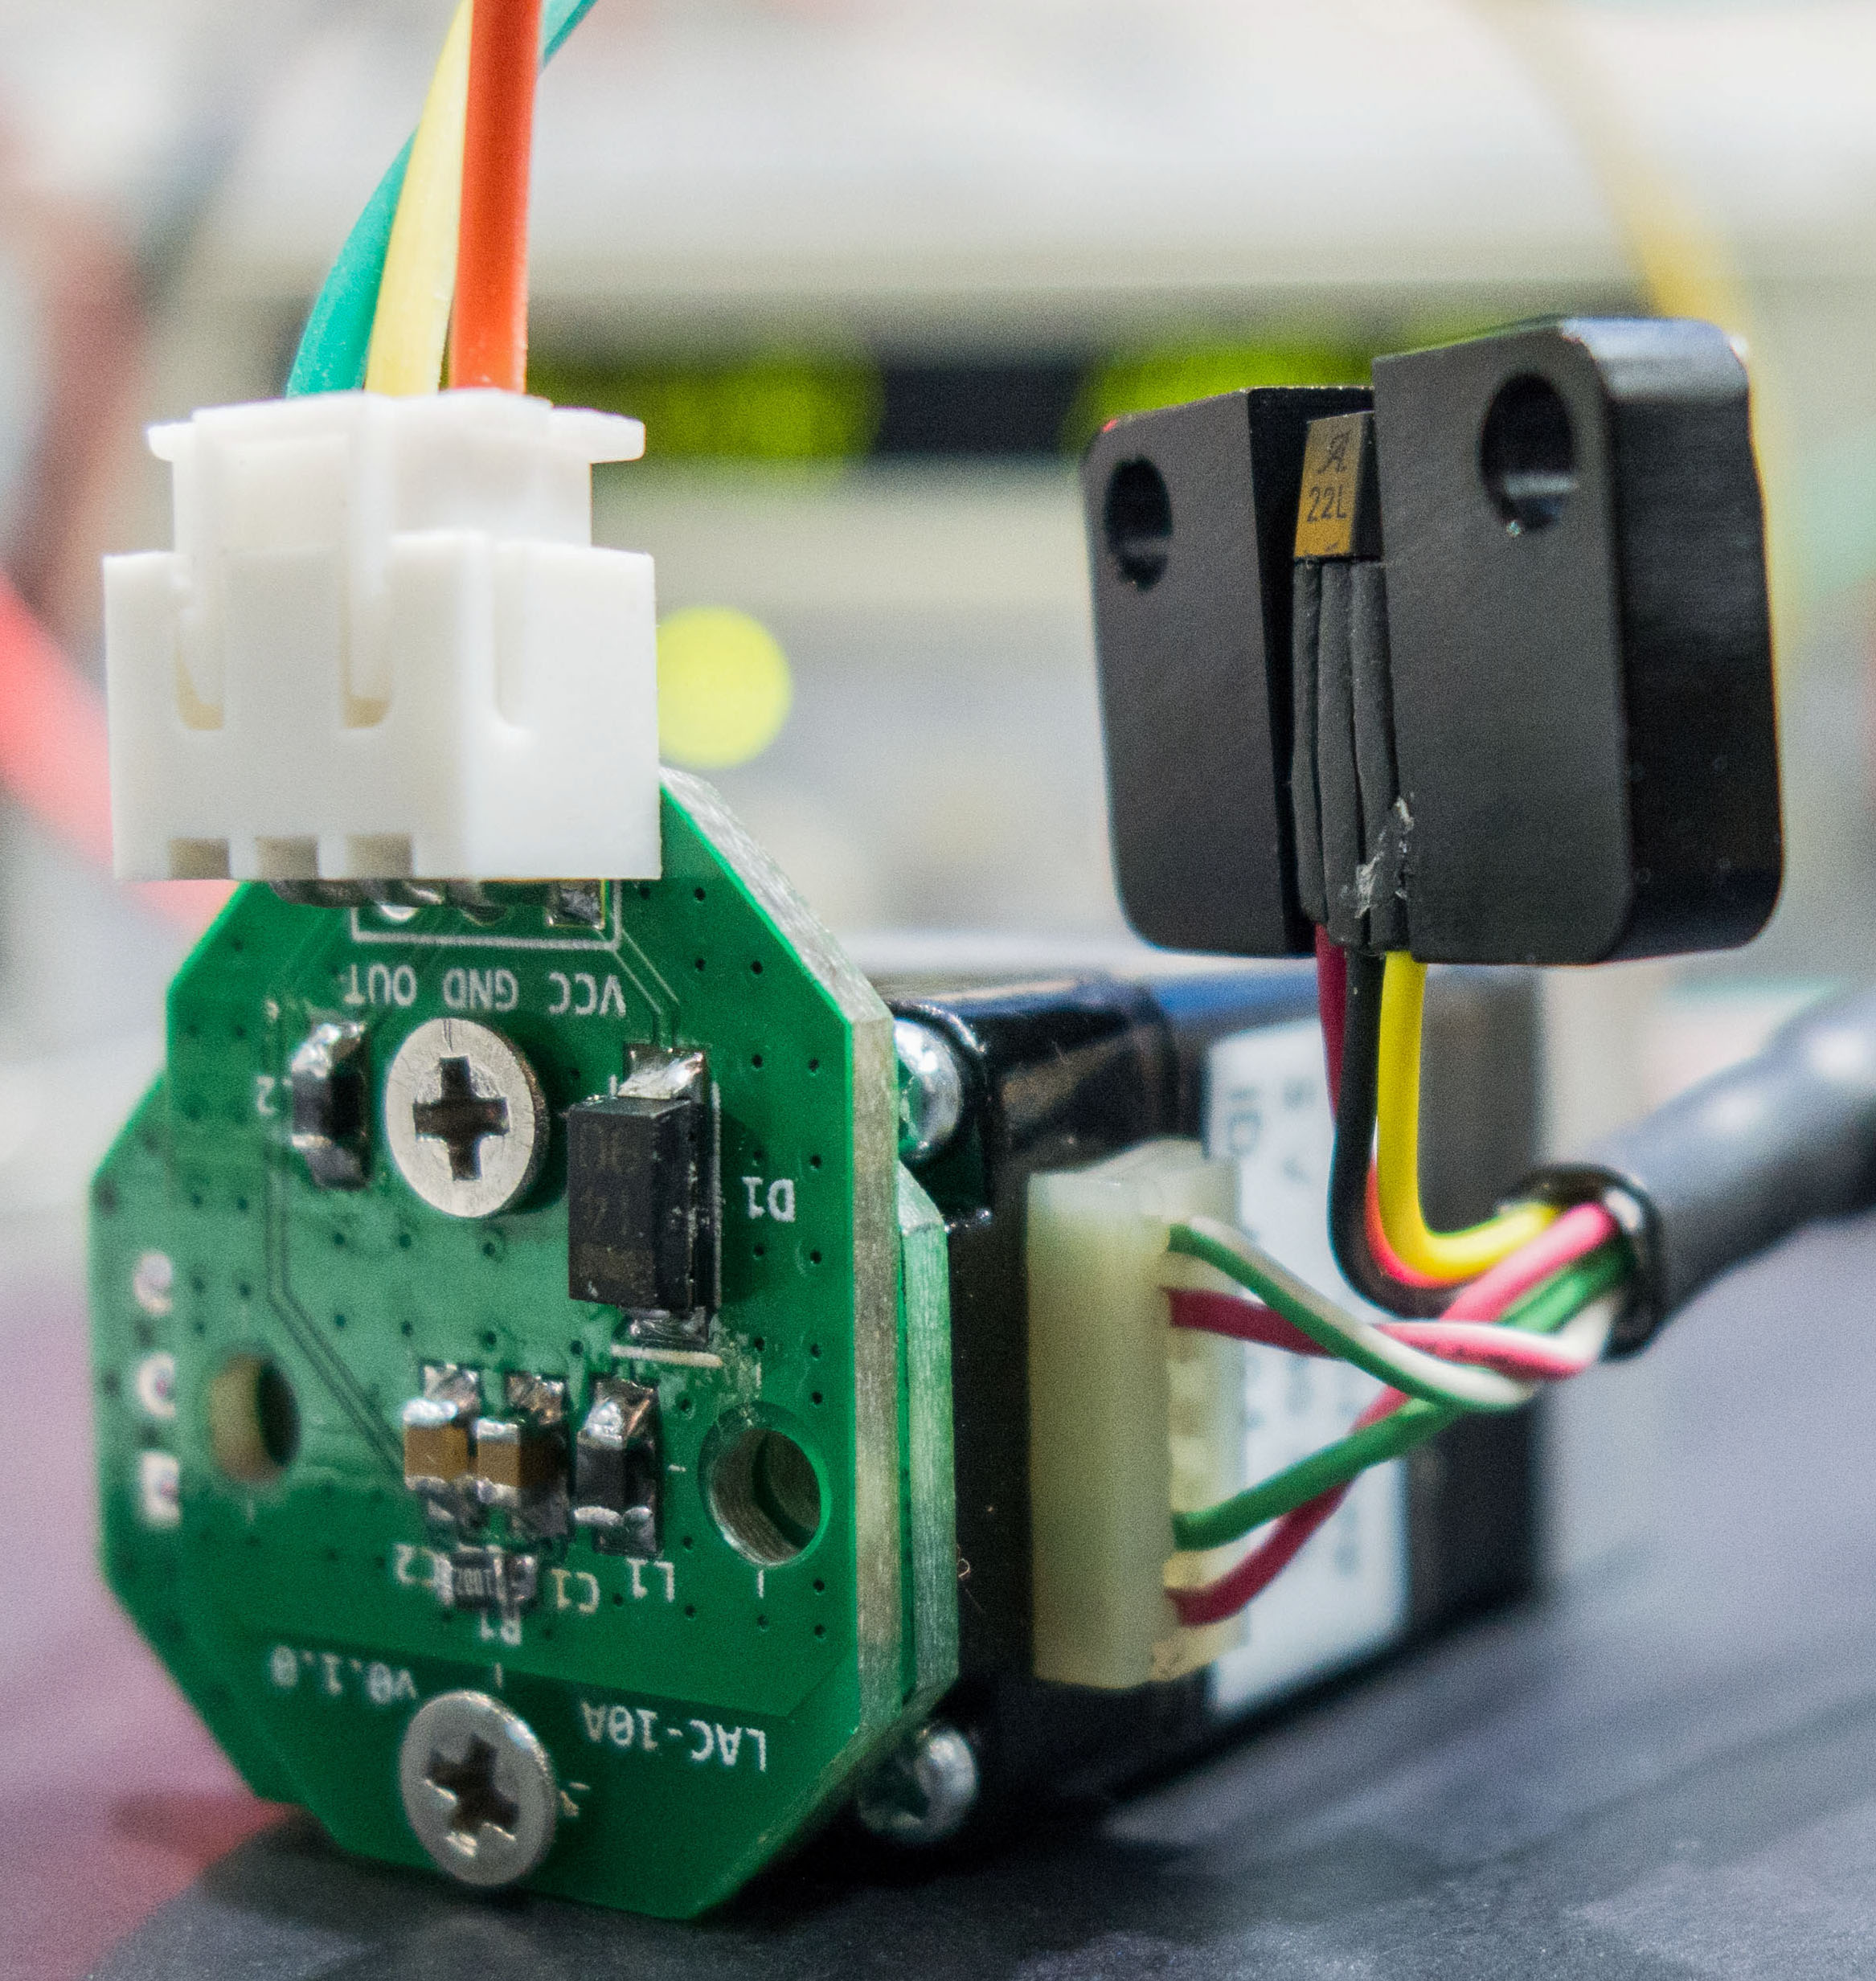
\includegraphics[height=0.50\textheight]{impl/pcb__zaber__new__photo.jpg}
\caption{LAC-10A零位传感器\csep 新设计\csep 实物图}
\label{fig:impl-pcb-zaber-new-photo}
\end{figure}


\clearpage


\subsection{微力探头组件整体联调}\label{sec:impl-pcb-probe}

在完成微力传感器接口(\ref{sec:impl-pcb-ad7730}节)与电动推杆接口(\ref{sec:impl-pcb-zaber}节)后,即可将整个微力探头组件接入MCU调试。首先按照\ref{sec:rig-ctrl-mcu-stepper}节步骤,在控制程序中实现电动推杆归零,实测通过;然后,将AD7730数据采集功能加入控制程序,确认采集到的微力传感器读数准确有效;最后,在程序中实现\ref{sec:rig-probe}节中的晶圆接触控制。经在硅片上测试(图~\ref{fig:impl-pcb-probe-touchdown}),初始接触力可控制在\SI{10}{\mN}以内,满足检测方案要求。

\begin{figure}[hb]
\centering
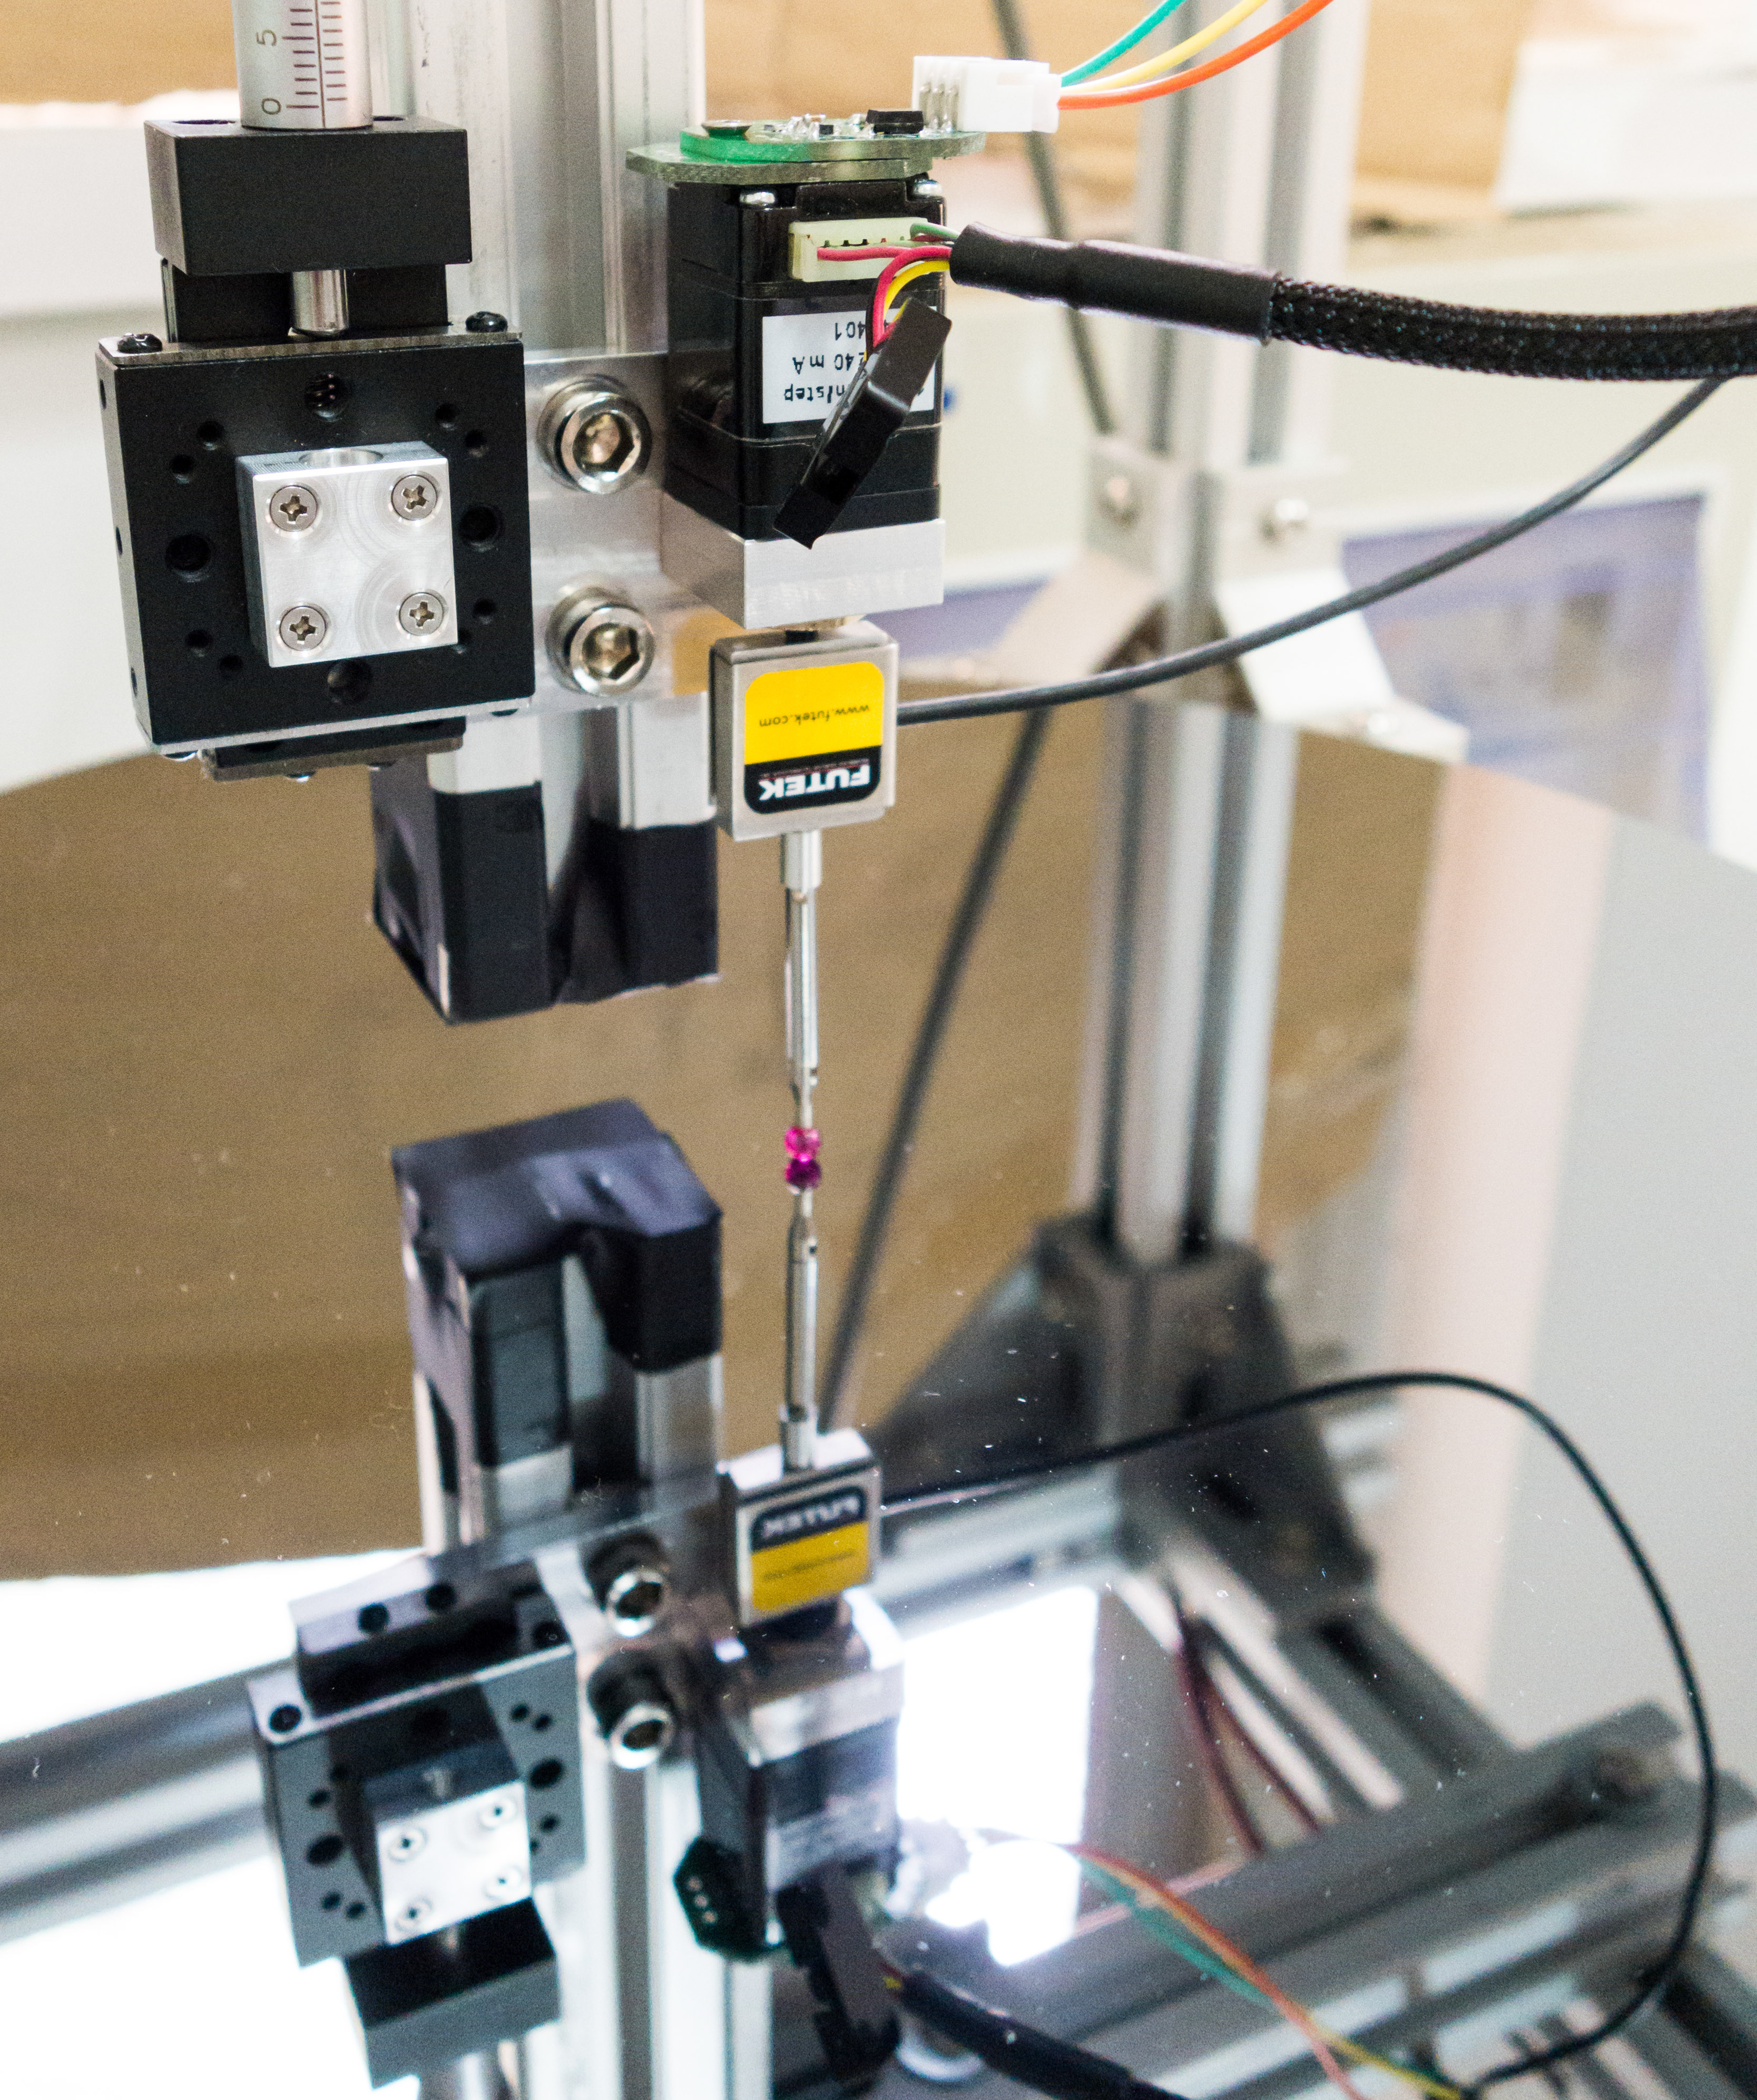
\includegraphics
  [max size={1\linewidth}{0.7\textheight}]
  {impl/pcb__probe__touchdown.jpg}
\caption{微力探头组件接触晶圆}
\label{fig:impl-pcb-probe-touchdown}
\end{figure}


\subsection{配电与接线}\label{sec:impl-pcb-power}

检测平台中,多处需要\SI{+24}{\V}或\SI{\pm 15}{\V}直流供电,可由两个开关电源提供。由\ref{sec:impl-pcb-pressure}节讨论知,还需接入\SI{+24}{\V}直流电源滤波器,将噪声源与噪声敏感电路隔离开。为方便检测平台的搭建与扩展,使用安装在DIN导轨上的接线端子块辅助配电,如图~\ref{fig:impl-pcb-power-terminal}。接线端子块从右至左依次分配为:交流\SI{220}{\V}市电(包括地线``FG'',在此处单点接地),\SI{+24}{\V}直流(未滤波、已滤波),\SI{\pm 15}{\V}直流。

电控系统中的MCU部分选用STM32F103VET6最小系统板(图~\ref{fig:impl-pcb-mcu}),按照\ref{sec:rig-ctrl-mcu}节中的针脚分配图将MCU与其他电路连接,形成电控系统的底层硬件部分,整体如图~\ref{fig:impl-pcb-overall}。

\begin{figure}[h]
\centering
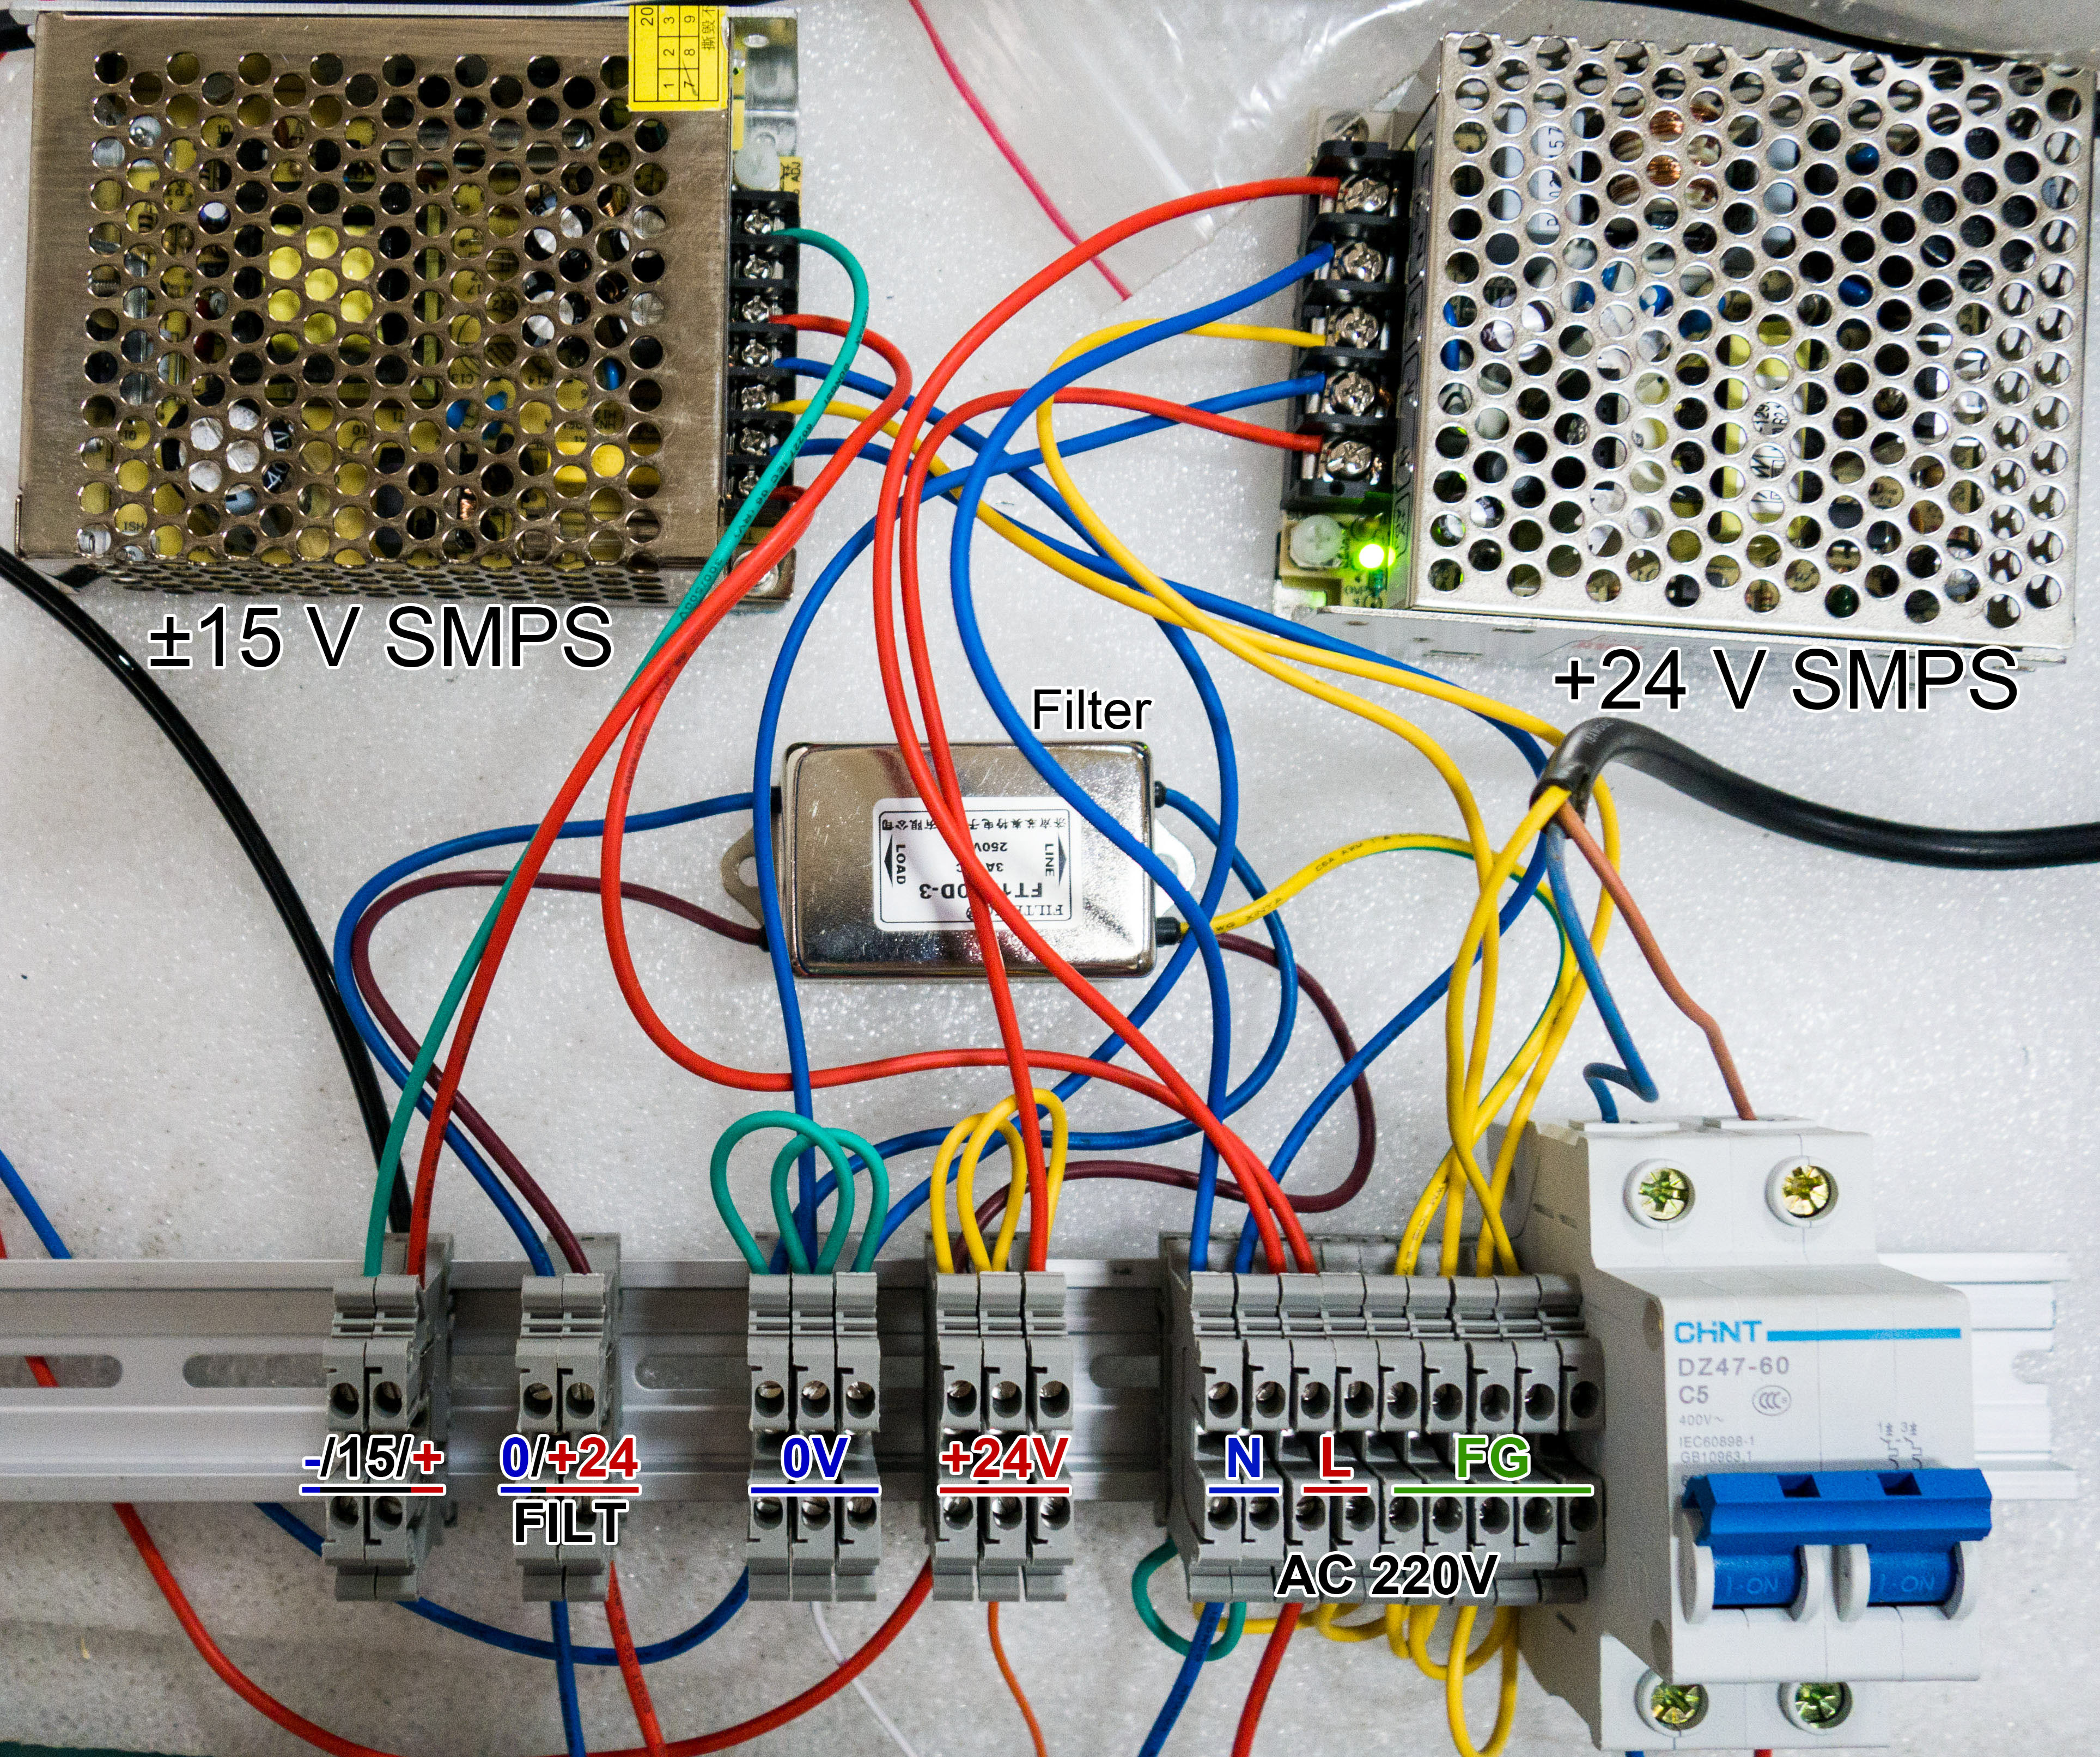
\includegraphics
  [max size={1\linewidth}{0.60\textheight}]
  {impl/pcb__power__terminal.jpg}
\caption{配电与接线端子实物图}
\label{fig:impl-pcb-power-terminal}
\end{figure}

\begin{figure}[hp]
\centering
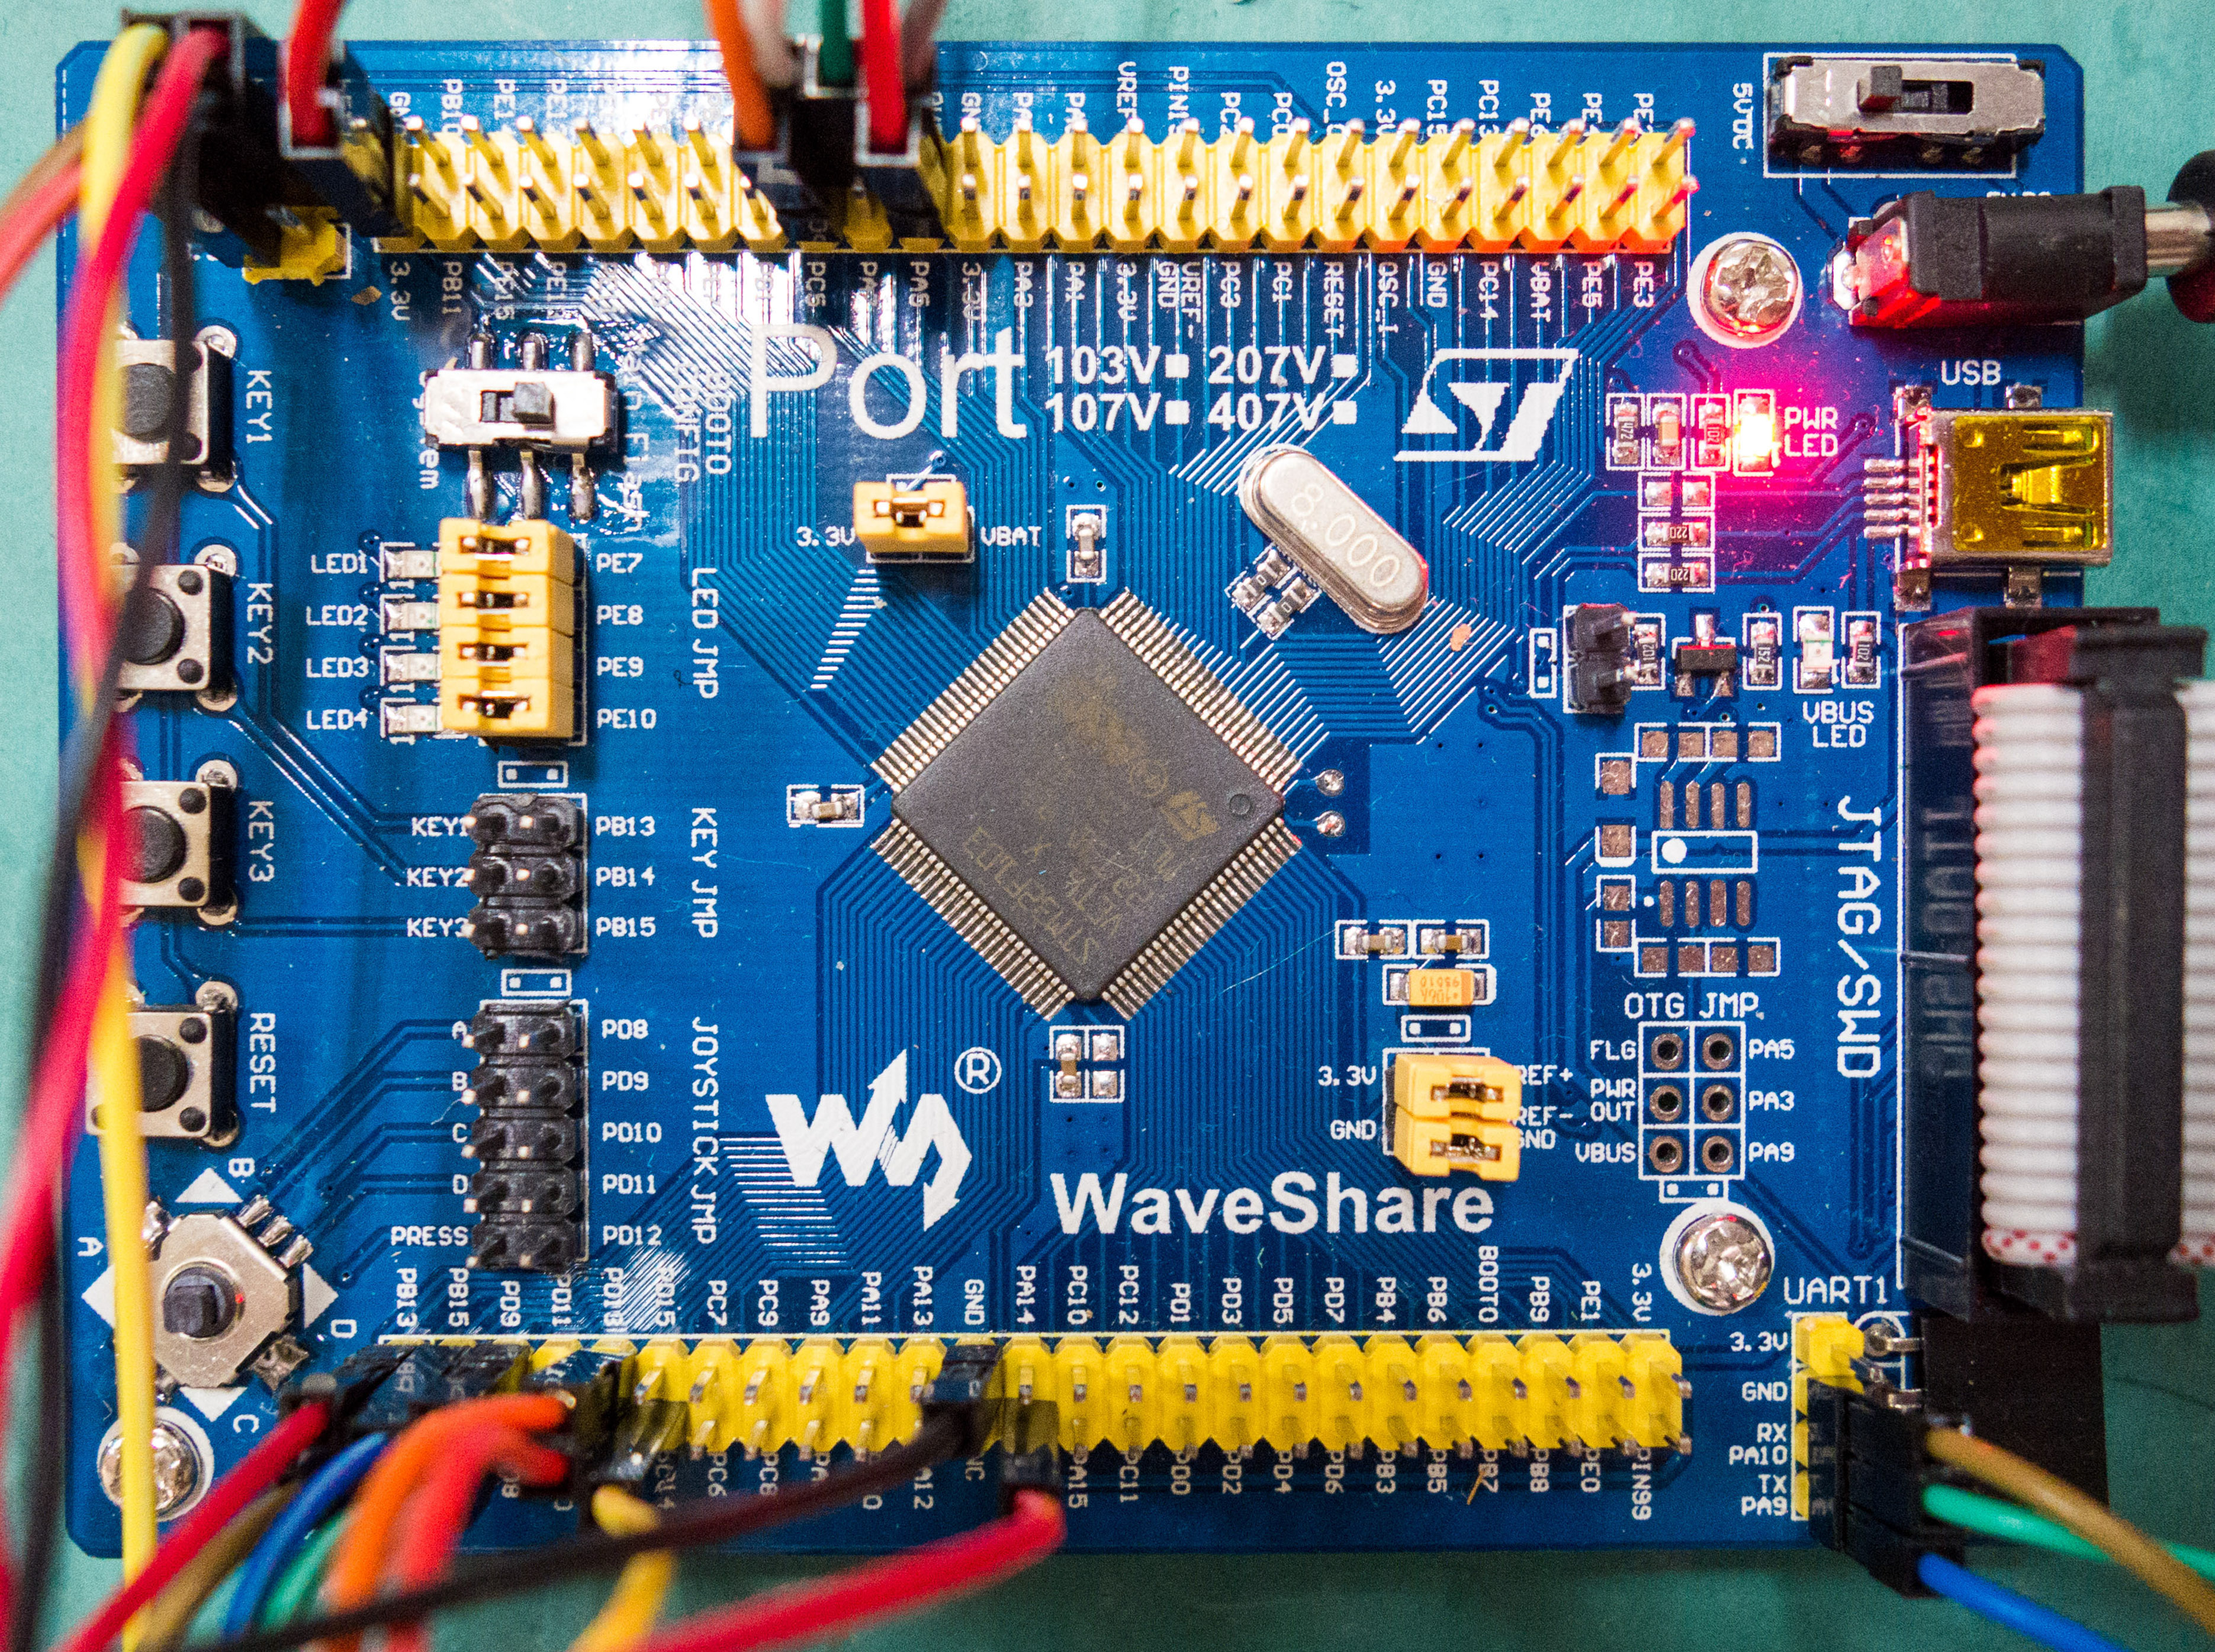
\includegraphics
  [max size={1\linewidth}{0.40\textheight}]
  {impl/pcb__mcu.jpg}
\caption{MCU最小系统板实物图}
\label{fig:impl-pcb-mcu}
\end{figure}

\begin{figure}[hp]
\centering
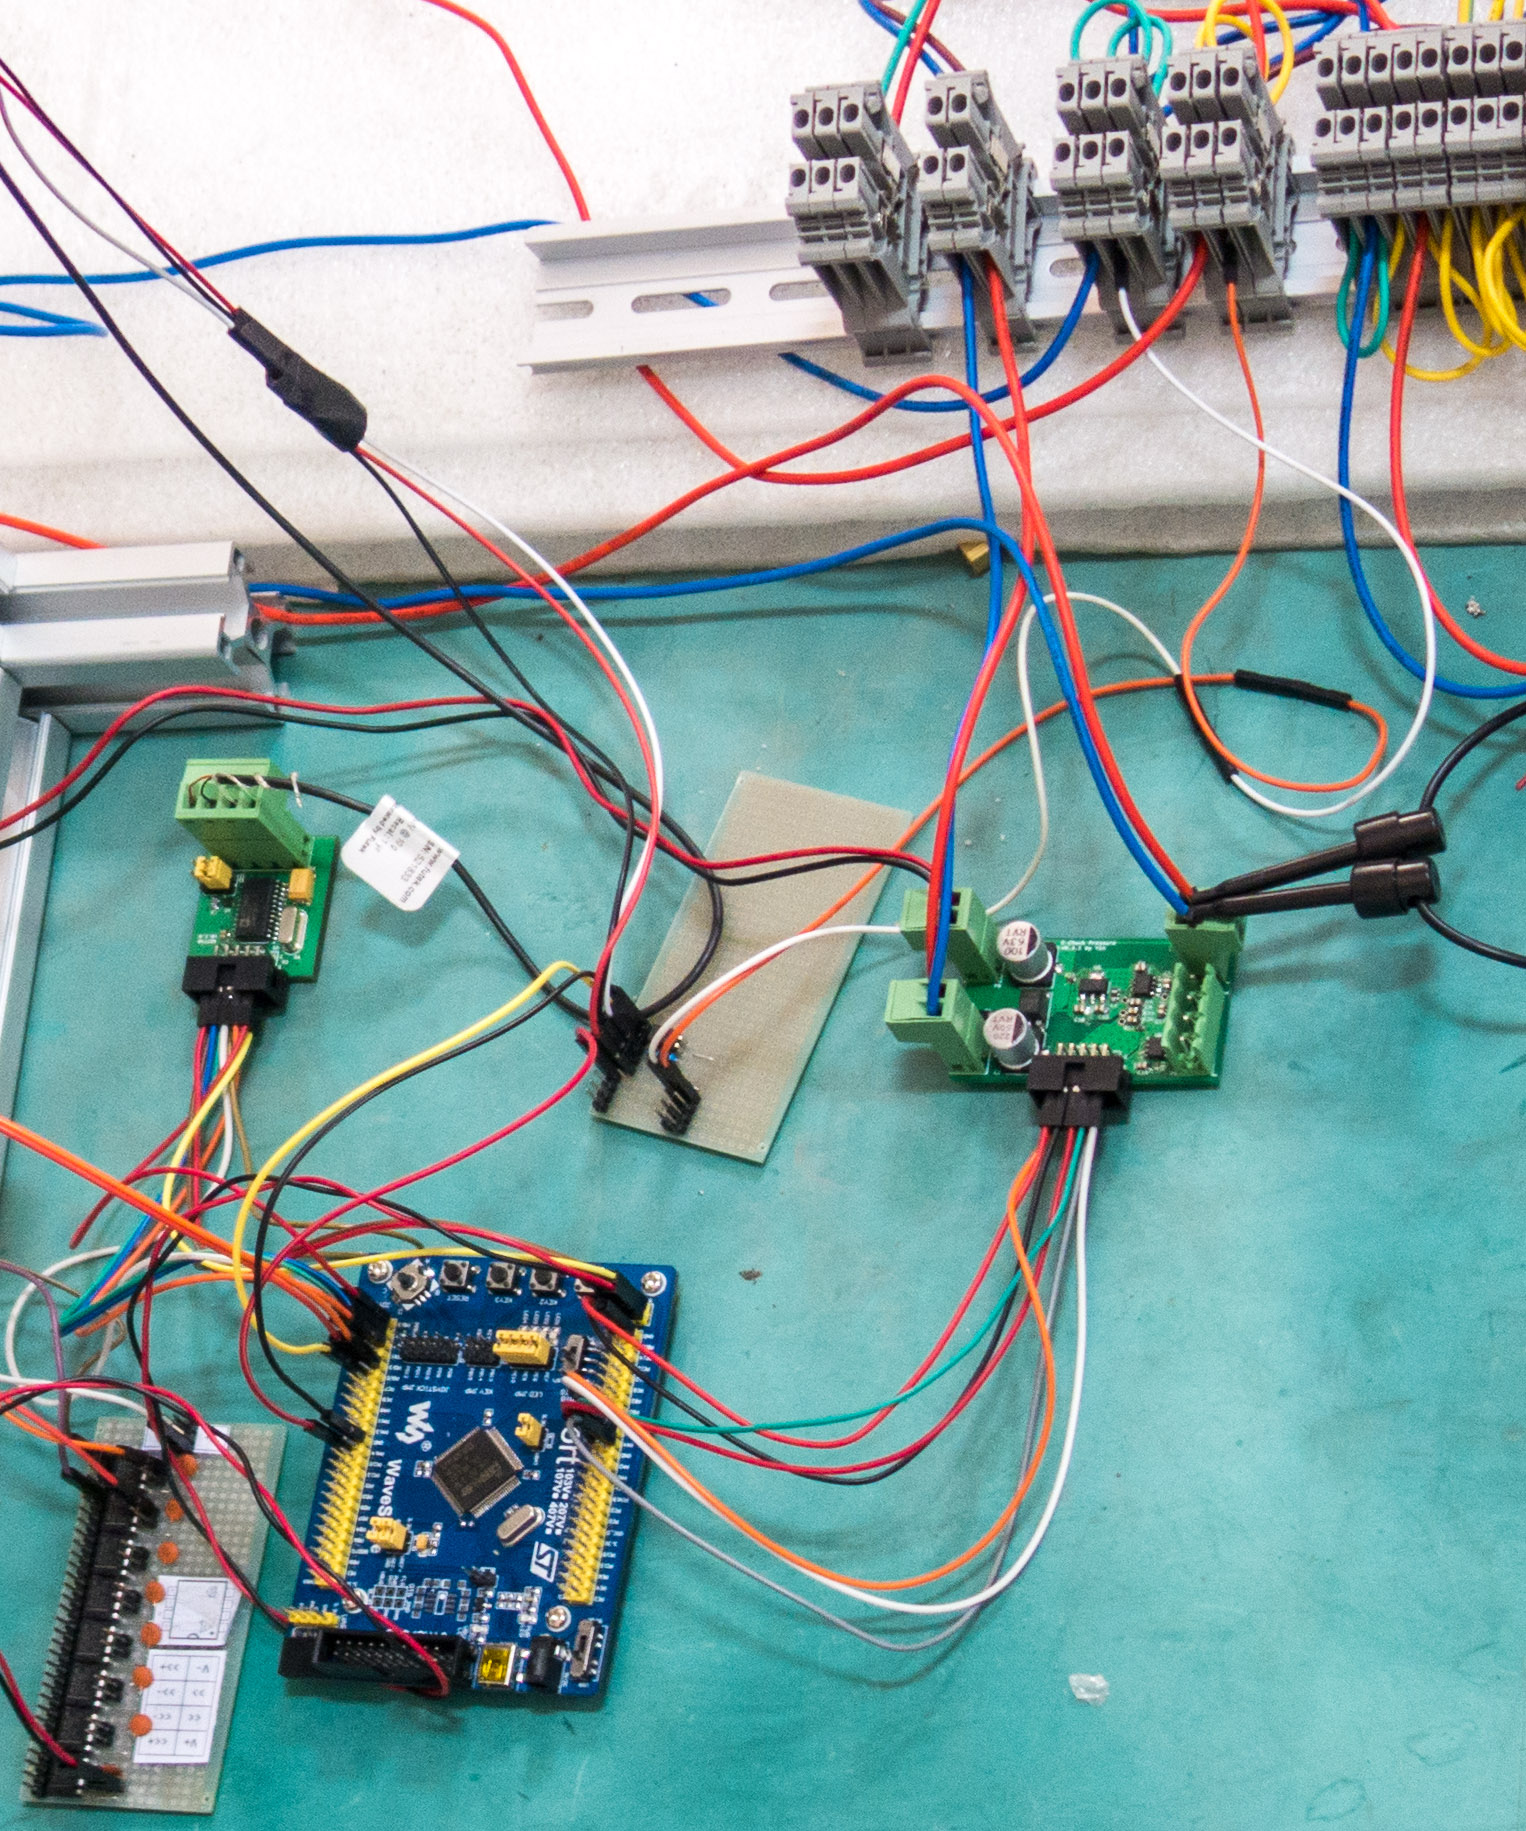
\includegraphics
  [max size={1\linewidth}{0.50\textheight}]
  {impl/pcb__overall.jpg}
\caption{电控系统硬件实物图}
\label{fig:impl-pcb-overall}
\end{figure}



\clearpage



\section{背吹控制系统搭建与调试}\label{sec:impl-pressure}

根据\ref{sec:rig-pressure}节中提出的背吹控制系统的供压、传感方案,综合考虑成本、时间等限制条件,确定实际搭建的背吹控制系统,如图~\ref{fig:impl-pressure-sch-full}、表~\ref{tab:impl-pressure-choice}:气源经过滤减压(未画出)后,依次经过两位三通电磁阀(\ref{sec:rig-pressure-valve}节)、精密机械减压阀(\ref{sec:rig-pressure-supply-reg}节)、电子比例阀(\ref{sec:rig-pressure-supply-integrated}节),接入静电卡盘背吹通道与压强变送器(\ref{sec:rig-pressure-sensor}节)。电子比例阀可选装:安装时,精密机械减压阀用于保证其入口压强不超过额定范围,并减小气源压强波动影响;不安装时,直接由精密机械减压阀向静电卡盘供压。另外,若需加装质量流量计/质量流量控制器(MFM/MFC),由于其两端存在一定压降,应将其串联在压强变送器连接点之前,以确保压强变送器测量的始终是背吹通道入口处压强。

\begin{figure}[h]
\centering
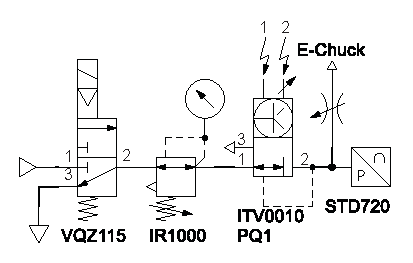
\includegraphics[width=0.618\linewidth]{impl/pressure__sch__full}
\caption{背吹控制系统\csep 总体气路图}
\label{fig:impl-pressure-sch-full}
\end{figure}

\begin{table}[h]
\centering
\caption{背吹控制系统核心件清单}
\label{tab:impl-pressure-choice}
\begin{minipage}{1\linewidth}
\centering
\begin{tabular}{cccSSc}

\toprule[1.5pt]
公司 & 型号 & 类型 & \multicolumn{2}{c}{压强/\si{\kPa}} & {流量/(\si{\liter\per\minute})} \\
\cmidrule{4-5}
&&& 最低 & 最高 & \\
\midrule[1pt]
SMC & VQZ115 & 两位三通电磁阀\footnotemark{} & 150 & 700 & \\
SMC & IR1000 & 精密机械减压阀 & 5 & 200 & 250 \\
SMC & ITV0010-3 & 电子比例阀 & 1 & 100 & 3.5 \\
Aircom & PQ1EE-C2 & 电子比例阀 & 0 & 20 & 35 \\
Honeywell & STD720 & 压强变送器 & -100 & +100\footnotemark{} & \\
\bottomrule[1.5pt]

\end{tabular}
\footnotetext{VQZ115为先导式电磁阀;直动式电磁阀反应速度更快,但受制于货期未能选用。}
\footnotetext{量程可在此范围内自由配置,见\ref{sec:rig-pressure-sensor}节。}
\end{minipage}
\end{table}

依据以上气路设计,在检测平台上搭建背吹控制系统。配管统一使用Festo $\diameter 4$ PU软管以及相应的气动快装接头。首先安装供压部分,如图~\ref{fig:impl-pressure-supply}:VQZ115体积较小,可直接串联在管路中,无需固定;IR1000可通过附带的连接板、T槽螺栓、法兰螺母固定在型材框架上;ITV0010直接使用附带的底座即可直立放置。接下来安装传感部分,如图~\ref{fig:impl-pressure-sense}:由于STD720自带液晶显示更新速率较慢,为方便调试,额外接入一个满量程\SI{16}{\kPa}的机械指针式压强计。实际测试时发现ITV0100允许的流量(\SI{3.5}{\liter\per\minute})过小,即使设定点为\SI{1}{\kPa}(标称最小值),仍无法保压;而替代产品PQ1货期较长,此时尚未到货,因此暂时将电子比例阀从背吹控制系统中移除。经实测,IR1000可输出低达\SI{0.25}{\kPa}的压强(该值随流量变化而变化,见\ref{sec:rig-pressure-supply-reg}节相关讨论),满足系统要求,可直接为背吹通道供压。

\begin{figure}[p]
\centering
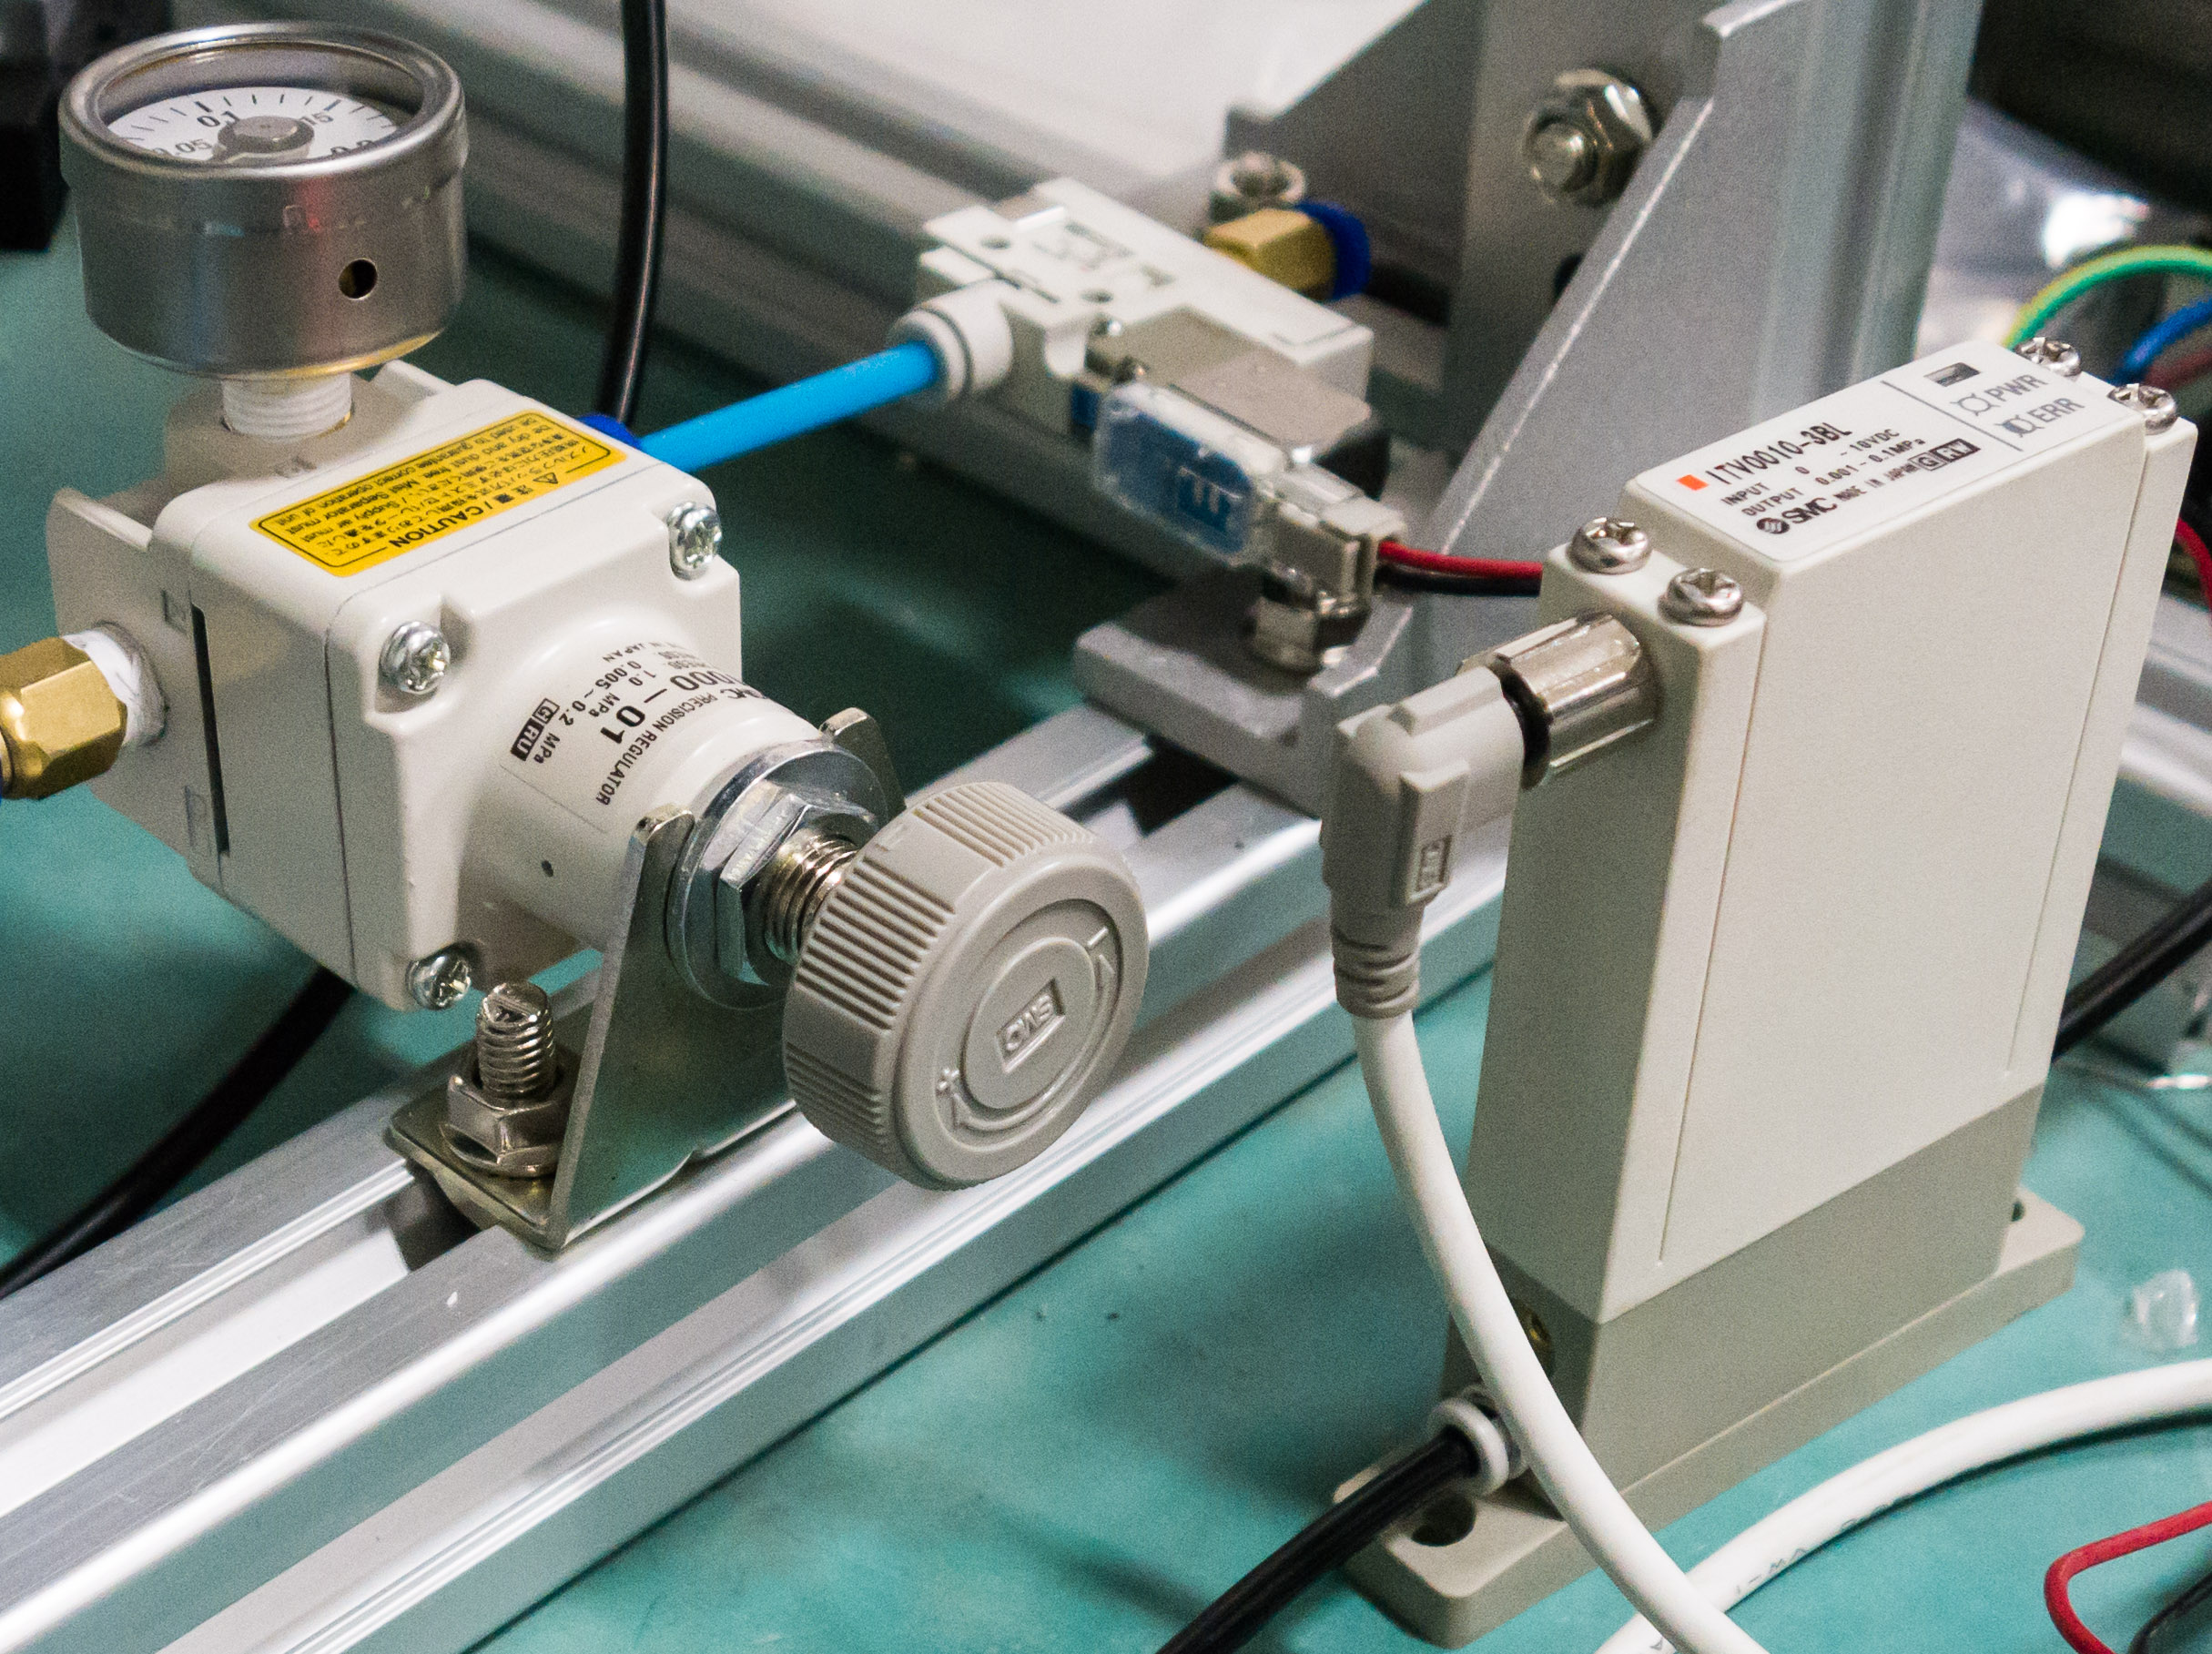
\includegraphics
  [max size={1\linewidth}{0.45\textheight}]
  {impl/pressure__supply__2.jpg}
\caption{背吹控制系统\csep 供压部分实物图}
\label{fig:impl-pressure-supply}
\end{figure}

\begin{figure}[p]
\centering
\includegraphics
  [max size={1\linewidth}{0.45\textheight}]
  {impl/pressure__sense.jpg}
\caption{背吹控制系统\csep 传感部分实物图}
\label{fig:impl-pressure-sense}
\end{figure}



\section{本章小结}\label{sec:impl-summary}

%TODO:summary
(总之我装好了)







